\documentclass[]{book}
\usepackage{lmodern}
\usepackage{amssymb,amsmath}
\usepackage{ifxetex,ifluatex}
\usepackage{fixltx2e} % provides \textsubscript
\ifnum 0\ifxetex 1\fi\ifluatex 1\fi=0 % if pdftex
  \usepackage[T1]{fontenc}
  \usepackage[utf8]{inputenc}
\else % if luatex or xelatex
  \ifxetex
    \usepackage{mathspec}
  \else
    \usepackage{fontspec}
  \fi
  \defaultfontfeatures{Ligatures=TeX,Scale=MatchLowercase}
\fi
% use upquote if available, for straight quotes in verbatim environments
\IfFileExists{upquote.sty}{\usepackage{upquote}}{}
% use microtype if available
\IfFileExists{microtype.sty}{%
\usepackage{microtype}
\UseMicrotypeSet[protrusion]{basicmath} % disable protrusion for tt fonts
}{}
\usepackage[margin=1in]{geometry}
\usepackage{hyperref}
\hypersetup{unicode=true,
            pdfborder={0 0 0},
            breaklinks=true}
\urlstyle{same}  % don't use monospace font for urls
\usepackage{natbib}
\bibliographystyle{apalike}
\usepackage{longtable,booktabs}
\usepackage{graphicx,grffile}
\makeatletter
\def\maxwidth{\ifdim\Gin@nat@width>\linewidth\linewidth\else\Gin@nat@width\fi}
\def\maxheight{\ifdim\Gin@nat@height>\textheight\textheight\else\Gin@nat@height\fi}
\makeatother
% Scale images if necessary, so that they will not overflow the page
% margins by default, and it is still possible to overwrite the defaults
% using explicit options in \includegraphics[width, height, ...]{}
\setkeys{Gin}{width=\maxwidth,height=\maxheight,keepaspectratio}
\IfFileExists{parskip.sty}{%
\usepackage{parskip}
}{% else
\setlength{\parindent}{0pt}
\setlength{\parskip}{6pt plus 2pt minus 1pt}
}
\setlength{\emergencystretch}{3em}  % prevent overfull lines
\providecommand{\tightlist}{%
  \setlength{\itemsep}{0pt}\setlength{\parskip}{0pt}}
\setcounter{secnumdepth}{5}
% Redefines (sub)paragraphs to behave more like sections
\ifx\paragraph\undefined\else
\let\oldparagraph\paragraph
\renewcommand{\paragraph}[1]{\oldparagraph{#1}\mbox{}}
\fi
\ifx\subparagraph\undefined\else
\let\oldsubparagraph\subparagraph
\renewcommand{\subparagraph}[1]{\oldsubparagraph{#1}\mbox{}}
\fi

%%% Use protect on footnotes to avoid problems with footnotes in titles
\let\rmarkdownfootnote\footnote%
\def\footnote{\protect\rmarkdownfootnote}

%%% Change title format to be more compact
\usepackage{titling}

% Create subtitle command for use in maketitle
\newcommand{\subtitle}[1]{
  \posttitle{
    \begin{center}\large#1\end{center}
    }
}

\setlength{\droptitle}{-2em}

  \title{}
    \pretitle{\vspace{\droptitle}}
  \posttitle{}
    \author{}
    \preauthor{}\postauthor{}
    \date{}
    \predate{}\postdate{}
  
\usepackage{booktabs}

\usepackage{amsthm}
\newtheorem{theorem}{Theorem}[chapter]
\newtheorem{lemma}{Lemma}[chapter]
\theoremstyle{definition}
\newtheorem{definition}{Definition}[chapter]
\newtheorem{corollary}{Corollary}[chapter]
\newtheorem{proposition}{Proposition}[chapter]
\theoremstyle{definition}
\newtheorem{example}{Example}[chapter]
\theoremstyle{definition}
\newtheorem{exercise}{Exercise}[chapter]
\theoremstyle{remark}
\newtheorem*{remark}{Remark}
\newtheorem*{solution}{Solution}
\begin{document}

{
\setcounter{tocdepth}{1}
\tableofcontents
}
\chapter*{Dear Residents,}\label{dear-residents}
\addcontentsline{toc}{chapter}{Dear Residents,}

We are pleased to present the 2018 edition of the Santa Barbara
Community Indicators Project (SBCIP). This is a revival of the South
Coast Community Indicators Project that ran for six editions from 1998
to 2003. The Santa Barbara Community Indicators Project incorporates
both North County and the South Coast in its measures, and is designed
to give an overall picture of our community's health and well-being.
This project was made possible through the financial support provided by
the Hutton-Parker Foundation, the Mosher Foundation, Montecito Bank \&
Trust, and the Gretler Foundation. The Santa Barbara Community
Indicators Project focuses on social, environmental, and economic data
within our community. The quality of our lives is a reflection of the
balance of social, environmental, and economic conditions. We encourage
our community to engage with us to discover ways in which we can
continually improve our health, safety and environment.

\chapter*{Introduction}\label{introduction}
\addcontentsline{toc}{chapter}{Introduction}

\section*{What is the Community Indicators
Project?}\label{what-is-the-community-indicators-project}
\addcontentsline{toc}{section}{What is the Community Indicators
Project?}

The Community Indicators Project is an effort to measure the social,
environmental, and economic factors that make up the quality of life in
our community. The project consists of the information in this report,
additional data provided at our website (www.efp.ucsb.edu), as well as
the process of generating the information. Both the product and the
process are essential elements of the effort. Our mission is:

\emph{To involve the Santa Barbara County community in developing and
using social, environmental, and economic indicators that will guide
decisions toward continually improving our quality of life.}

Each section contains the measures used to describe an issue, why those
measures are useful and how our community is doing with regard to those
measures. The data presented throughout this document cover a wide range
of topics and, when possible, separates North County from the South
Coast. This is done to better delineate the differences even within a
relatively small area. These data should help us discover where our
resources can be placed to reduce areas of concern. It is our hope that
policy makers and our citizenry will use the information here to better
our lives and well-being.

\chapter*{Social Indicators}\label{social-indicators}
\addcontentsline{toc}{chapter}{Social Indicators}

\section*{Demographics}\label{demographics}
\addcontentsline{toc}{section}{Demographics}

\subsubsection*{What are the measures?}\label{what-are-the-measures}
\addcontentsline{toc}{subsubsection}{What are the measures?}

Population growth and the distributions of Santa Barbara County by age,
gender, educational attainment, and race/ethnicity.

\subsubsection*{Why are they important?}\label{why-are-they-important}
\addcontentsline{toc}{subsubsection}{Why are they important?}

Population growth has a major impact on many aspects of life in Santa
Barbara County from economic growth to social and environmental
problems. Santa Barbara County residents of different ages require
different services. The racial and ethnic make-up of our community shows
an aspect of its diversity.

\subsubsection*{How are we doing?}\label{how-are-we-doing}
\addcontentsline{toc}{subsubsection}{How are we doing?}

Population growth in the Santa Barbara area has been very consistent
over the past 9, but has slowed to a slightly less than one percent
growth rate. The County growth rate was 0.72\% in 2015, and both North
and South County have followed a similar growth path in recent years.
The racial and ethnic profile of North County demonstrates a higher
Hispanic population than any other race or ethnic group. The South Coast
has a higher percentage of white citizens, followed by a substantial
number of Hispanic residents.

\begin{center}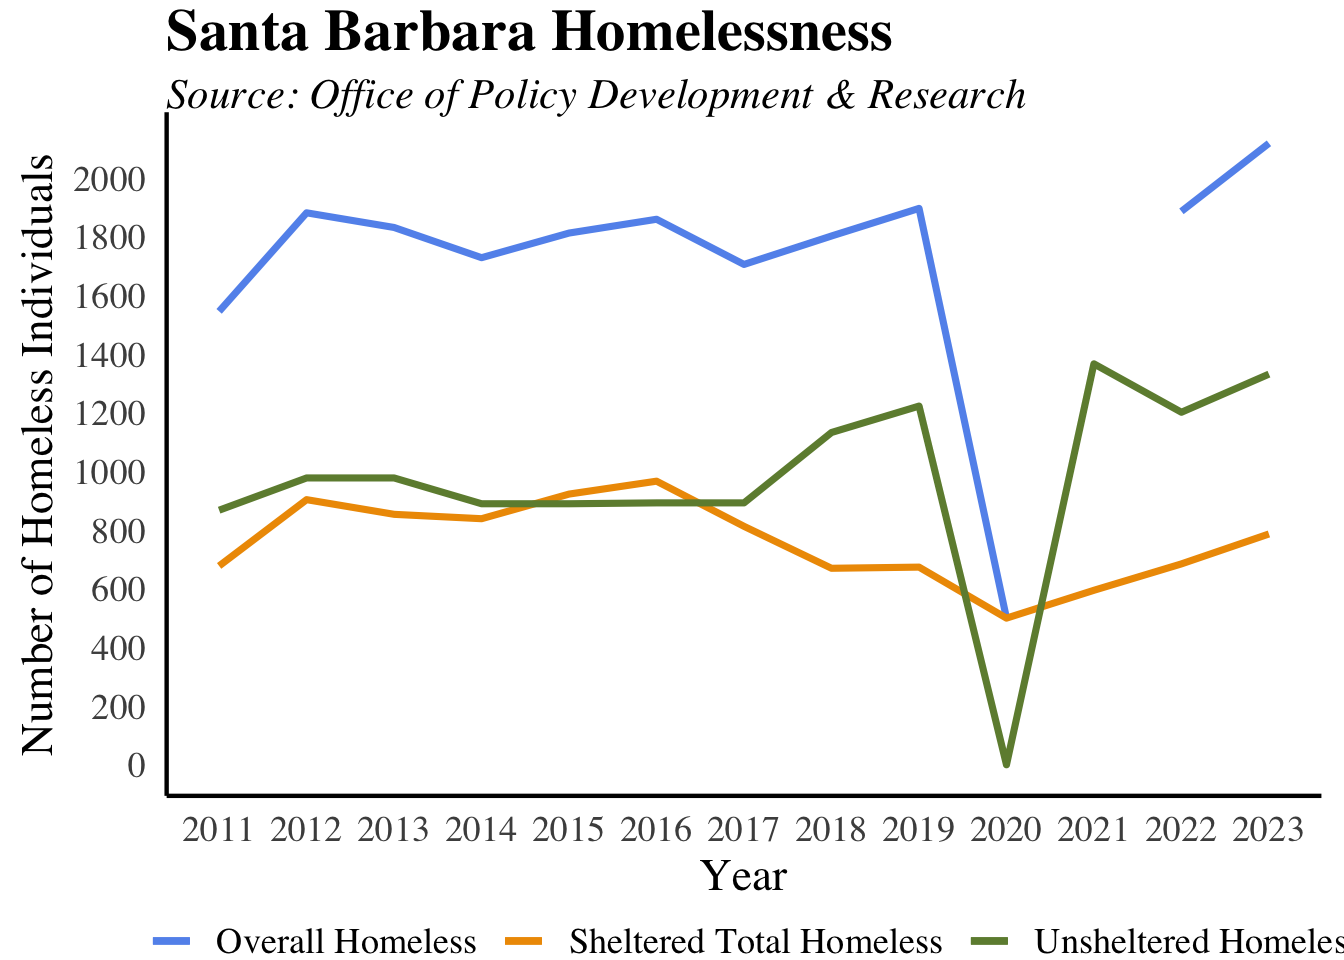
\includegraphics{cip_2019_files/figure-latex/unnamed-chunk-3-1} \end{center}

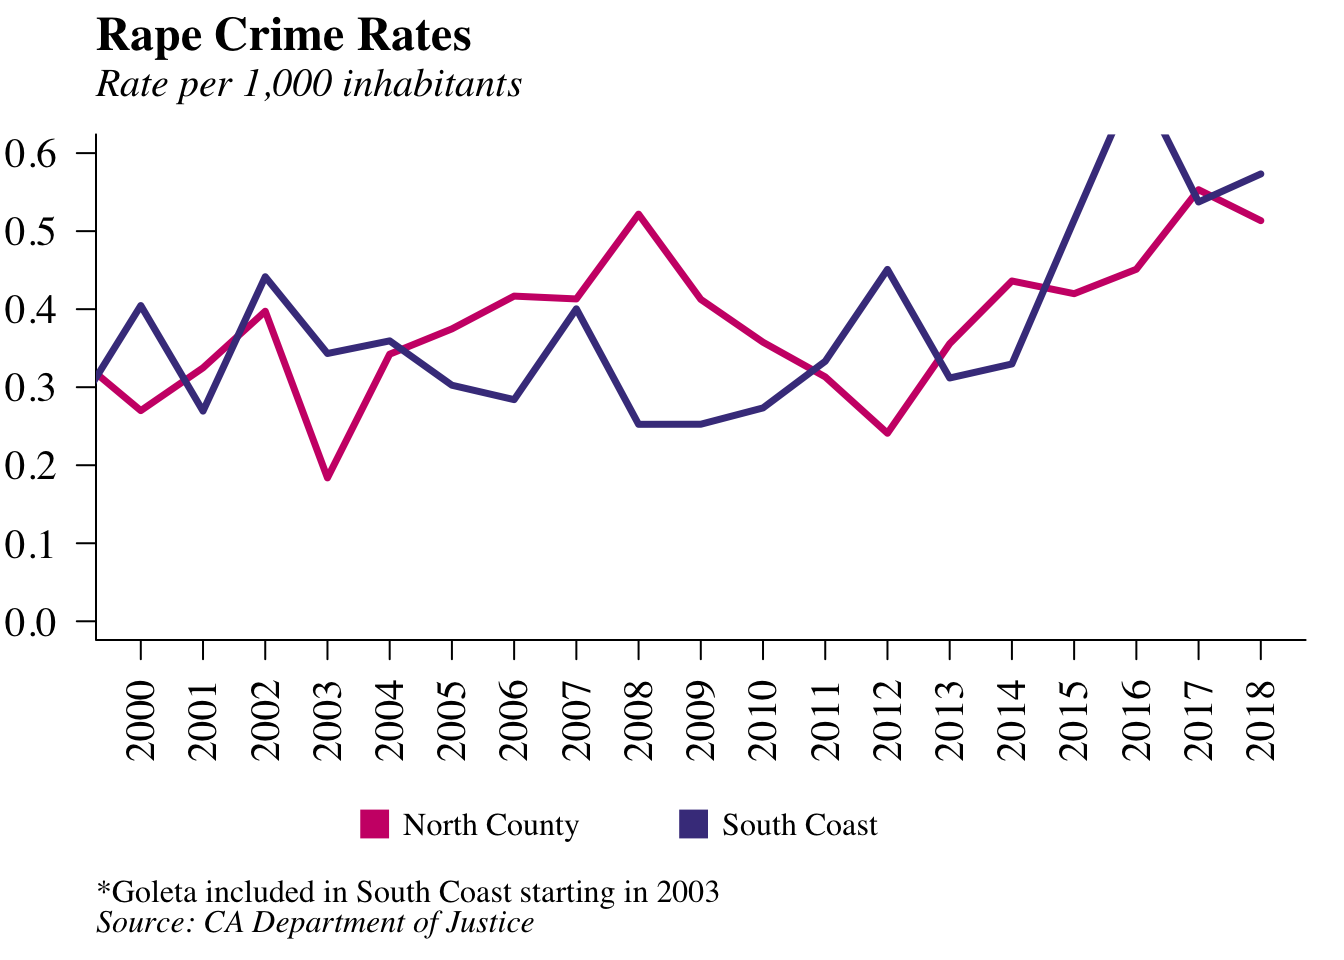
\includegraphics[width=0.45\linewidth]{cip_2019_files/figure-latex/unnamed-chunk-4-1}

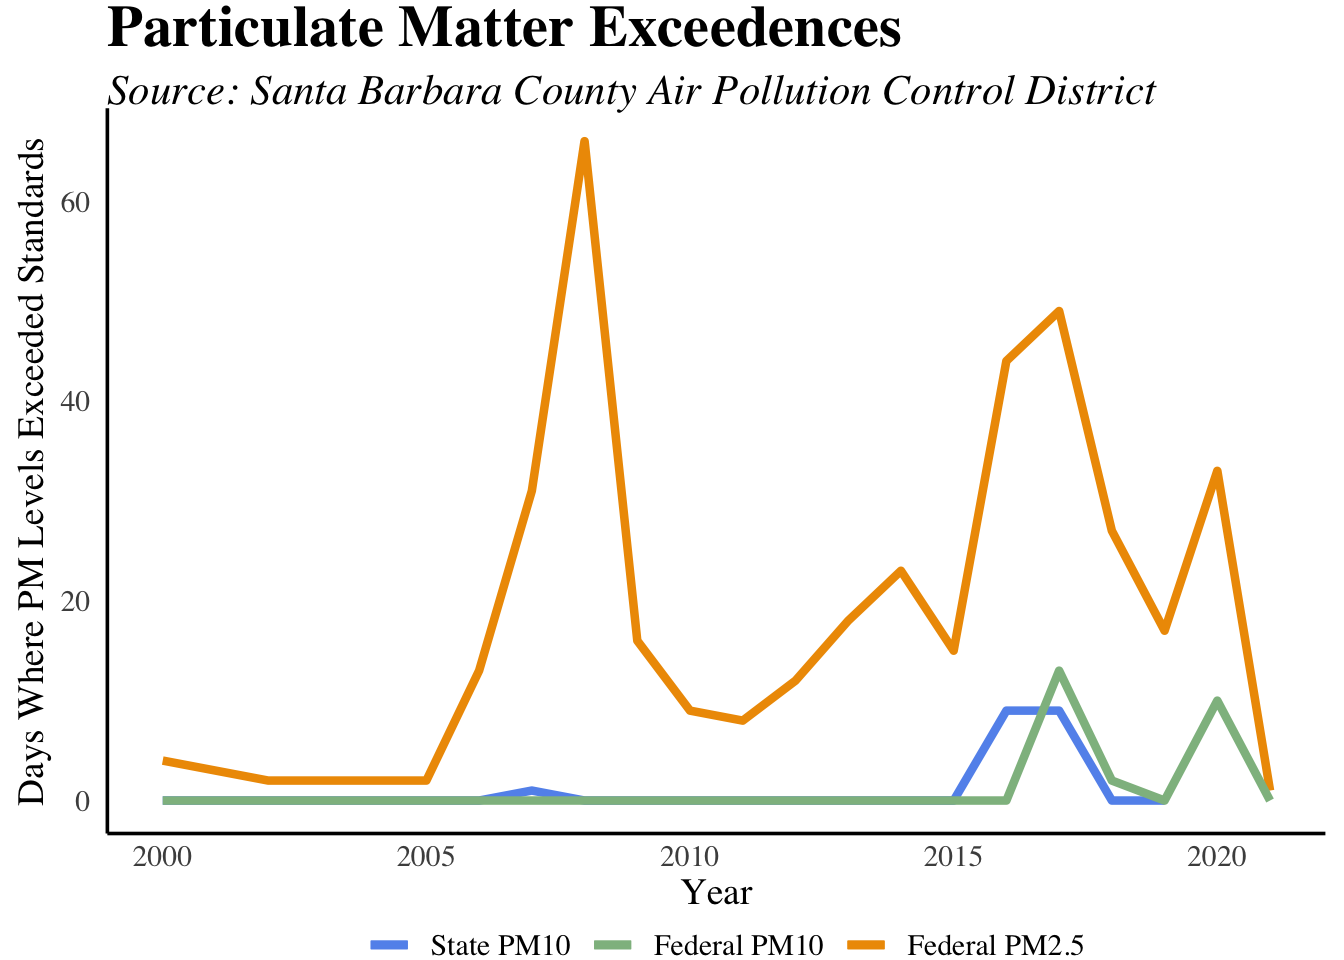
\includegraphics[width=0.45\linewidth]{cip_2019_files/figure-latex/unnamed-chunk-5-1}

\section*{Neighborhood and Community
Well-Being}\label{neighborhood-and-community-well-being}
\addcontentsline{toc}{section}{Neighborhood and Community Well-Being}

\subsubsection*{What are the measures?}\label{what-are-the-measures-1}
\addcontentsline{toc}{subsubsection}{What are the measures?}

These crime rates measure the number of property and violent crimes per
1,000 people in North County and in the South Coast. Violent crimes
include homicide, rape, robbery, and aggravated assault, whereas
property crimes include burglary, motor vehicle theft, and
larceny-theft.

\subsubsection*{Why are the measures
important?}\label{why-are-the-measures-important}
\addcontentsline{toc}{subsubsection}{Why are the measures important?}

Crime affects the level of real and perceived safety, which greatly
impacts the health of neighborhoods. In some cases, the reality and
perception of safety can be different.

\subsubsection*{How are we doing?}\label{how-are-we-doing-1}
\addcontentsline{toc}{subsubsection}{How are we doing?}

Violent crimes have fallen in both North County and the South Coast over
the last several years. This year, the violent crime reached an all-time
low of 2.65 crimes per 1,000 people for the South Coast, representing a
17 percent decrease from 2013 levels. After several years of having a
significantly higher crime rate than the South Coast, North County saw a
13 percent decrease in violent crime rates over the past year, with only
3.8 crimes per 1,000 people.

Property crime rates have also fallen over the past year for the South
Coast. The South Coast saw a 12 percent decrease, whereas North County
observed a 2 percent decrease.

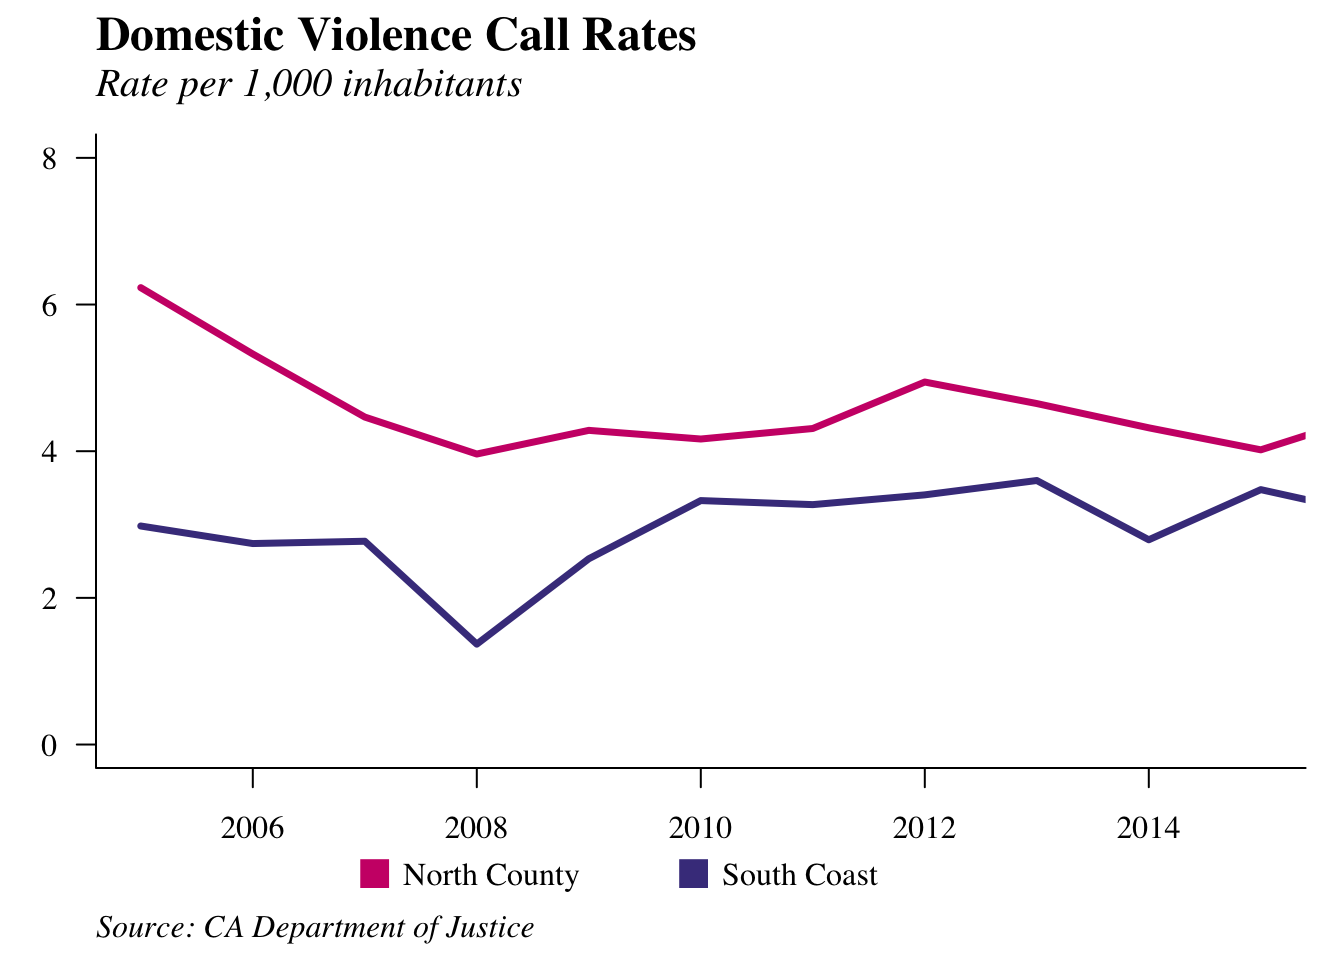
\includegraphics[width=0.95\linewidth]{cip_2019_files/figure-latex/unnamed-chunk-6-1}

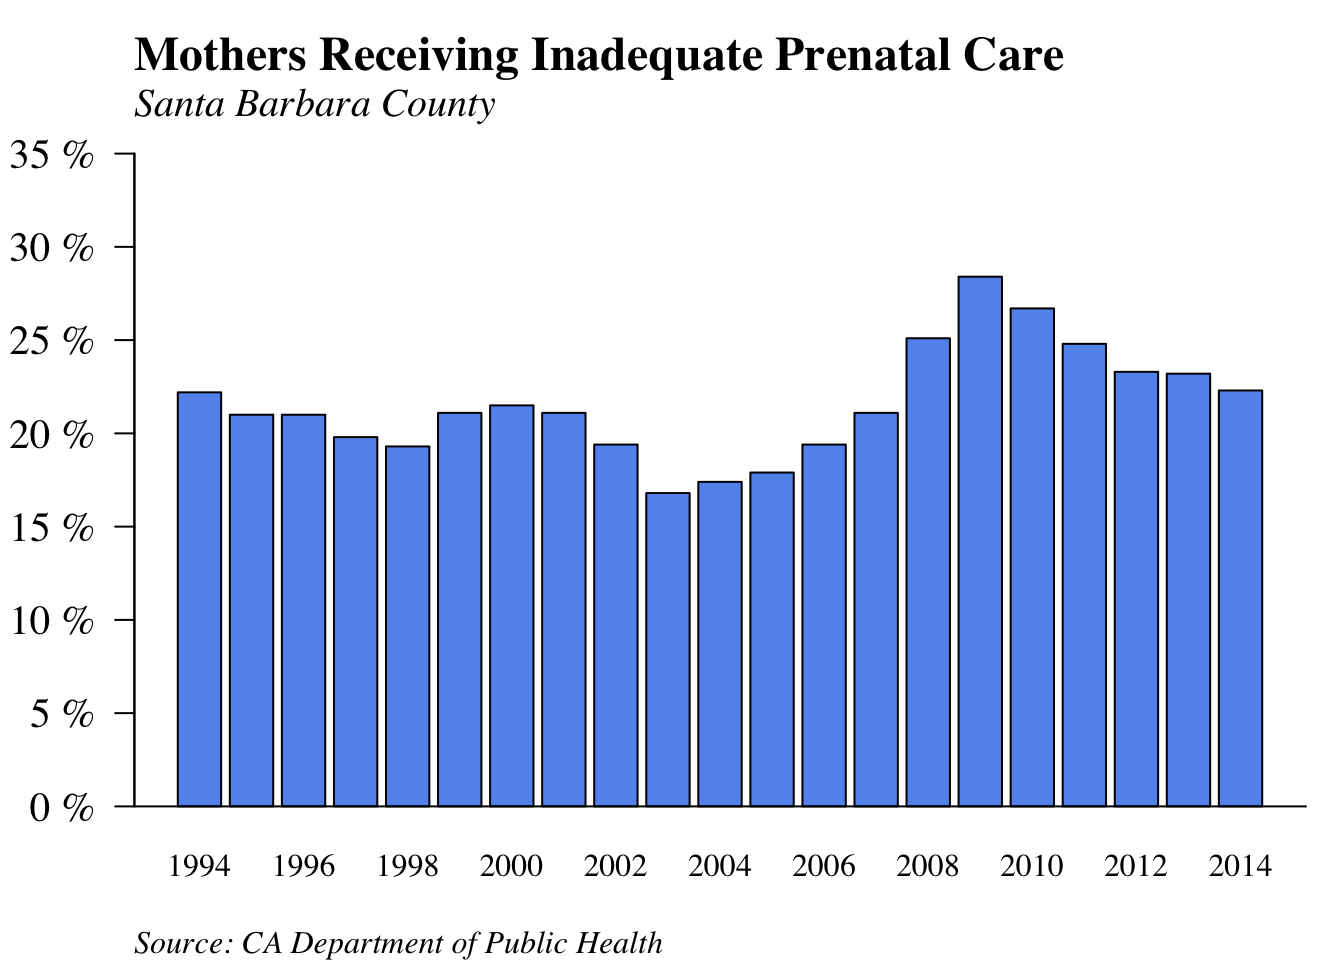
\includegraphics[width=0.95\linewidth]{cip_2019_files/figure-latex/unnamed-chunk-7-1}

\subsection*{JUVENILE FELONY ARRESTS NEAR LOWEST IN
DECADE}\label{juvenile-felony-arrests-near-lowest-in-decade}
\addcontentsline{toc}{subsection}{JUVENILE FELONY ARRESTS NEAR LOWEST IN
DECADE}

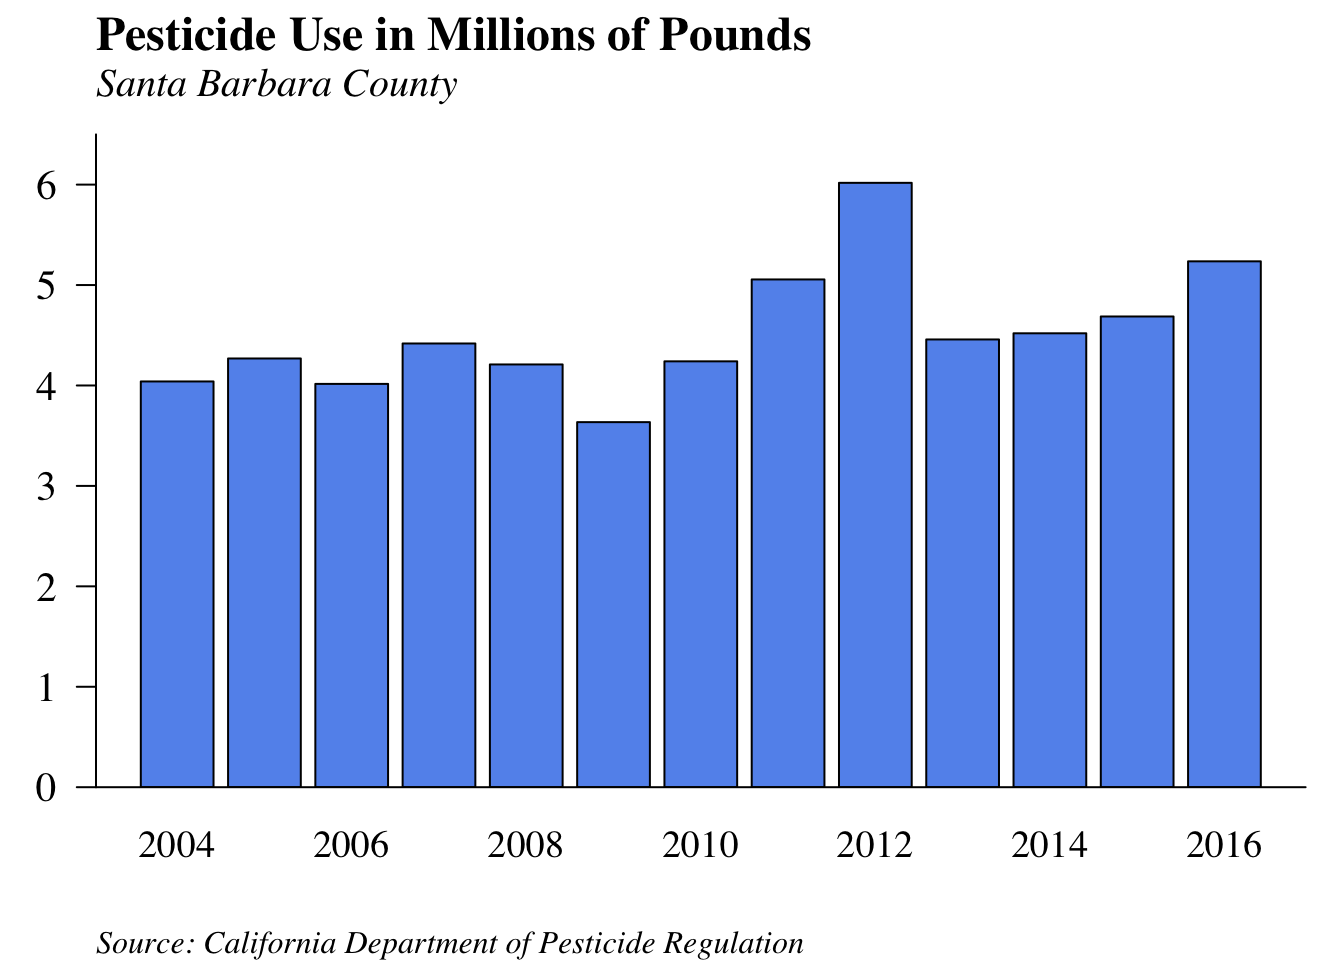
\includegraphics[width=0.95\linewidth]{cip_2019_files/figure-latex/unnamed-chunk-8-1}

\subsubsection*{What is the measure?}\label{what-is-the-measure}
\addcontentsline{toc}{subsubsection}{What is the measure?}

The number of juvenile felony arrests in Santa Barbara County per 1,000
people, including homicide, rape, aggravated assault, and larceny.

\subsubsection*{Why is it important?}\label{why-is-it-important}
\addcontentsline{toc}{subsubsection}{Why is it important?}

The rate of juvenile crime not only impacts our community's safety
today, but also gives us an indication of how safe our community may be
in the future. In addition, it reflects the effectiveness of
intervention programs focused at teens and pre-teens.

\subsubsection*{How are we doing?}\label{how-are-we-doing-2}
\addcontentsline{toc}{subsubsection}{How are we doing?}

Juvenile arrest rates have decreased over the last decade, reaching a
low of 7.6 arrests per 1,000 youth in 2013. The current rate is 7.7,
which is a 49 percent decrease from its level ten years ago.

\subsection*{CHILD MALTREATMENT ALLEGATIONS ON THE
RISE}\label{child-maltreatment-allegations-on-the-rise}
\addcontentsline{toc}{subsection}{CHILD MALTREATMENT ALLEGATIONS ON THE
RISE}

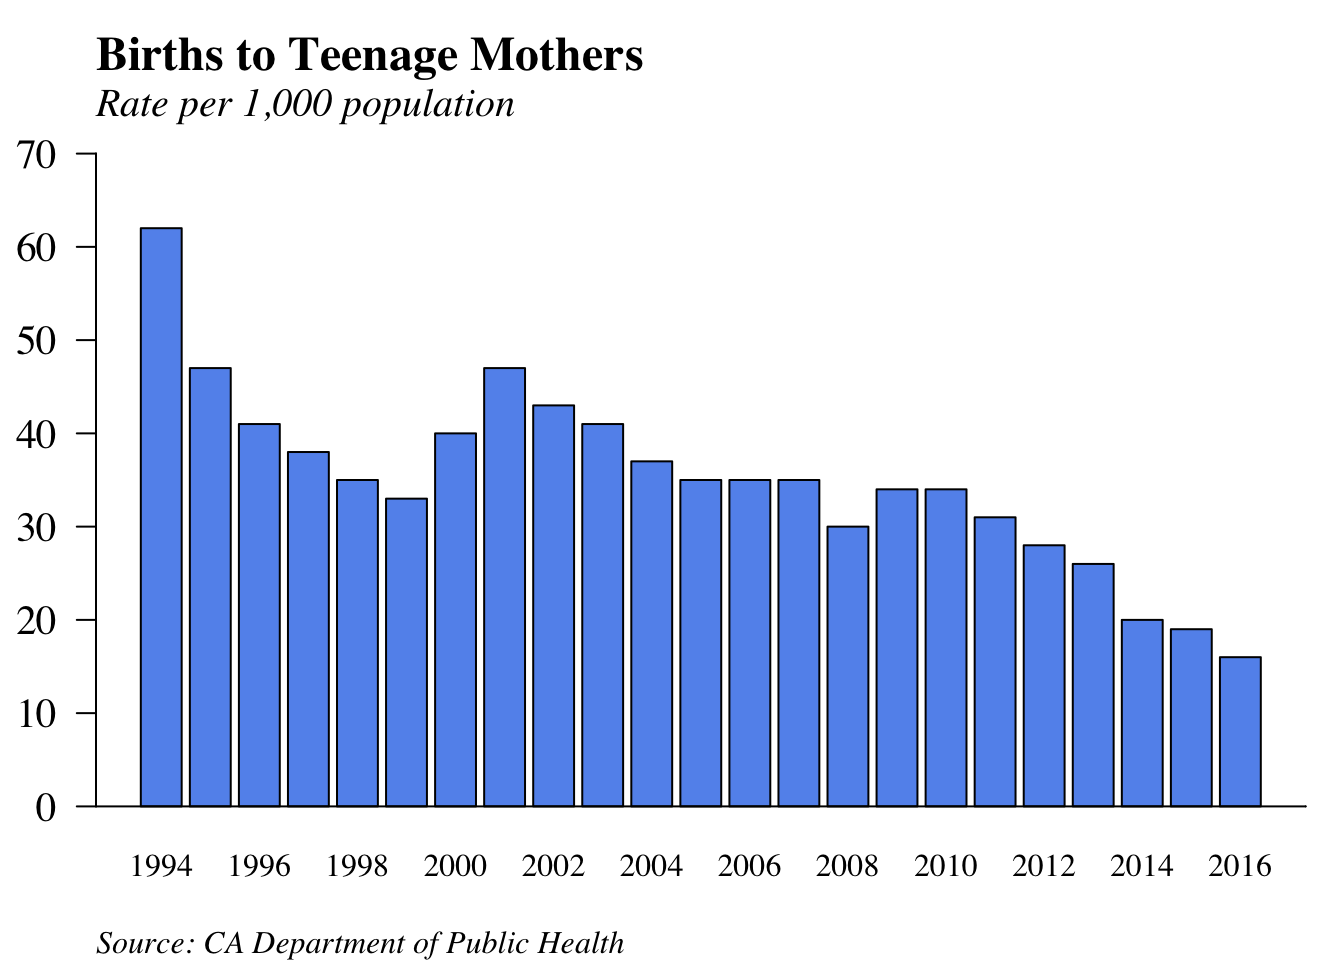
\includegraphics[width=0.95\linewidth]{cip_2019_files/figure-latex/unnamed-chunk-9-1}

\subsubsection*{What is the measure?}\label{what-is-the-measure-1}
\addcontentsline{toc}{subsubsection}{What is the measure?}

The number of children in Santa Barbara County with at least one child
maltreatment allegation, which includes sexual, emotional, and physical
abuse, severe and general neglect, exploitation, caretaker
absence/incapacity, and at risk allegations. If a child has more than
one allegation in different categories, the child is only counted once.

\subsubsection*{Why is it important?}\label{why-is-it-important-1}
\addcontentsline{toc}{subsubsection}{Why is it important?}

This is the best measure summarizing all types of child abuse and
neglect encountered within the community. The consequence of child abuse
impacts not only the child but on support services and school systems as
well.

\subsubsection*{How are we doing?}\label{how-are-we-doing-3}
\addcontentsline{toc}{subsubsection}{How are we doing?}

In 2015, Santa Barbara County surpassed its previous peak in child
maltreatment allegations with 5,533 cases. Child maltreatment
allegations have consistently been on the rise since 2010.

\section*{Individual and Family
Well-Being}\label{individual-and-family-well-being}
\addcontentsline{toc}{section}{Individual and Family Well-Being}

\subsection*{DOMESTIC VIOLENCE CALL RATE DECREASES
SLIGHTLY}\label{domestic-violence-call-rate-decreases-slightly}
\addcontentsline{toc}{subsection}{DOMESTIC VIOLENCE CALL RATE DECREASES
SLIGHTLY}

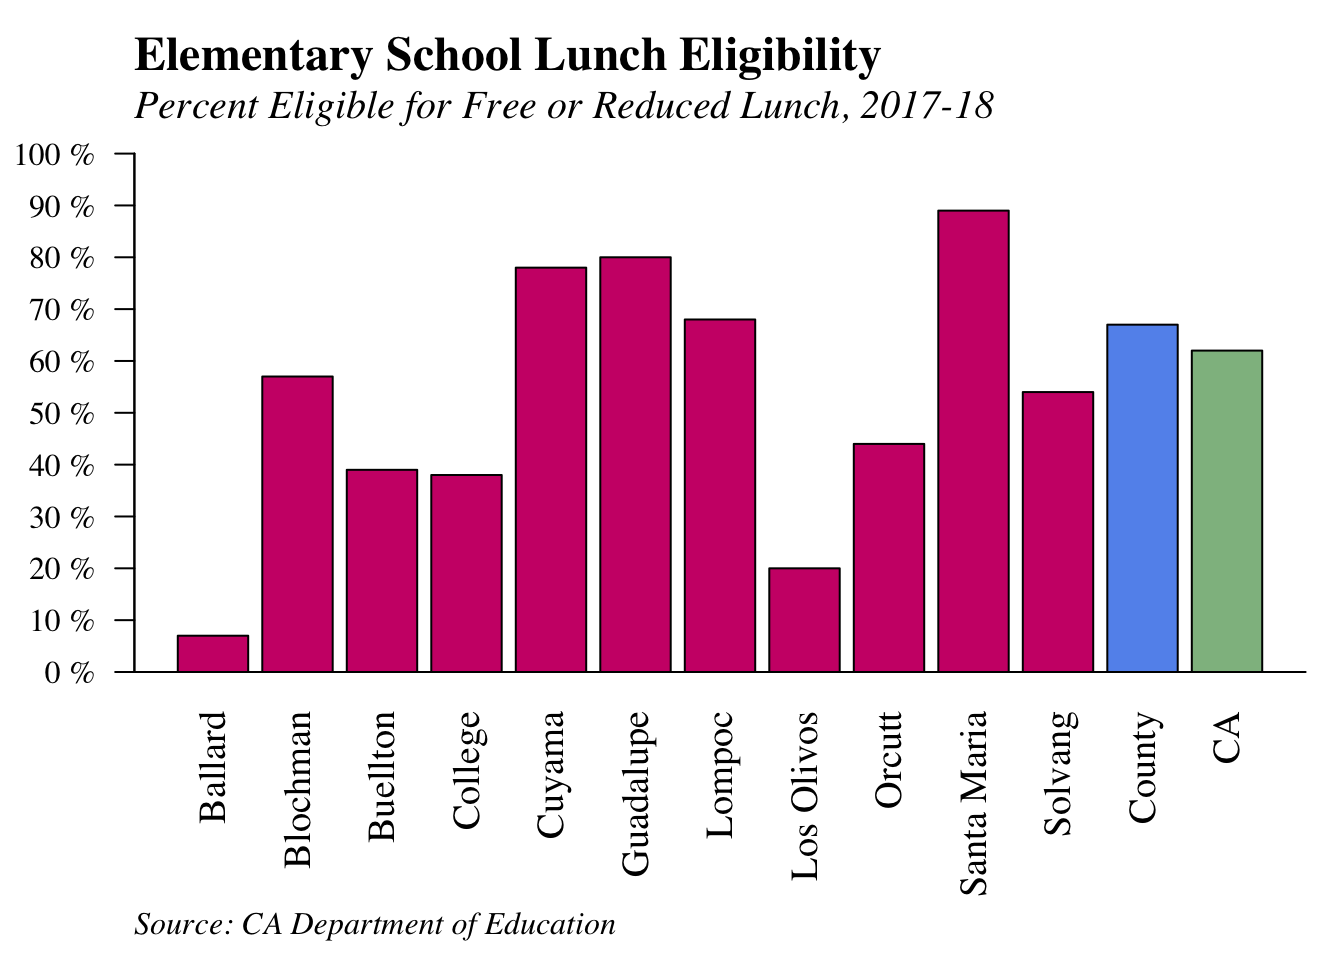
\includegraphics[width=0.95\linewidth]{cip_2019_files/figure-latex/unnamed-chunk-10-1}

\subsubsection*{What is the measure?}\label{what-is-the-measure-2}
\addcontentsline{toc}{subsubsection}{What is the measure?}

The domestic violence call rate is the number of 911 calls reported to
police and sheriff departments in Santa Barbara County regarding
domestic violence, including violence to children. This measure includes
attacks with guns, knives, heavy objects, hands, fists, and feet. In
order to control for growth in population, it is defined as the rate of
calls per 1,000 people.

\subsubsection*{Why is it important?}\label{why-is-it-important-2}
\addcontentsline{toc}{subsubsection}{Why is it important?}

Domestic violence has tragic implications for the individual health and
wellbeing of adults and children, and directly impacts the families to
which they belong. Domestic violence may also be an indicator of the
relative health of a community as a whole.

\subsubsection*{How are we doing?}\label{how-are-we-doing-4}
\addcontentsline{toc}{subsubsection}{How are we doing?}

The domestic violence call rate decreased by 0.28 calls for North County
and increased by 0.71 calls for the South Coast per 1,000 people in the
past year. Both North County and South Coast experienced their lowest
rate in 2008 at 3.9 and 1.4 calls per 1,000 people, respectively.

\subsection*{WEAPON-RELATED DOMESTIC VIOLENCE CALLS
CONSTANT}\label{weapon-related-domestic-violence-calls-constant}
\addcontentsline{toc}{subsection}{WEAPON-RELATED DOMESTIC VIOLENCE CALLS
CONSTANT}

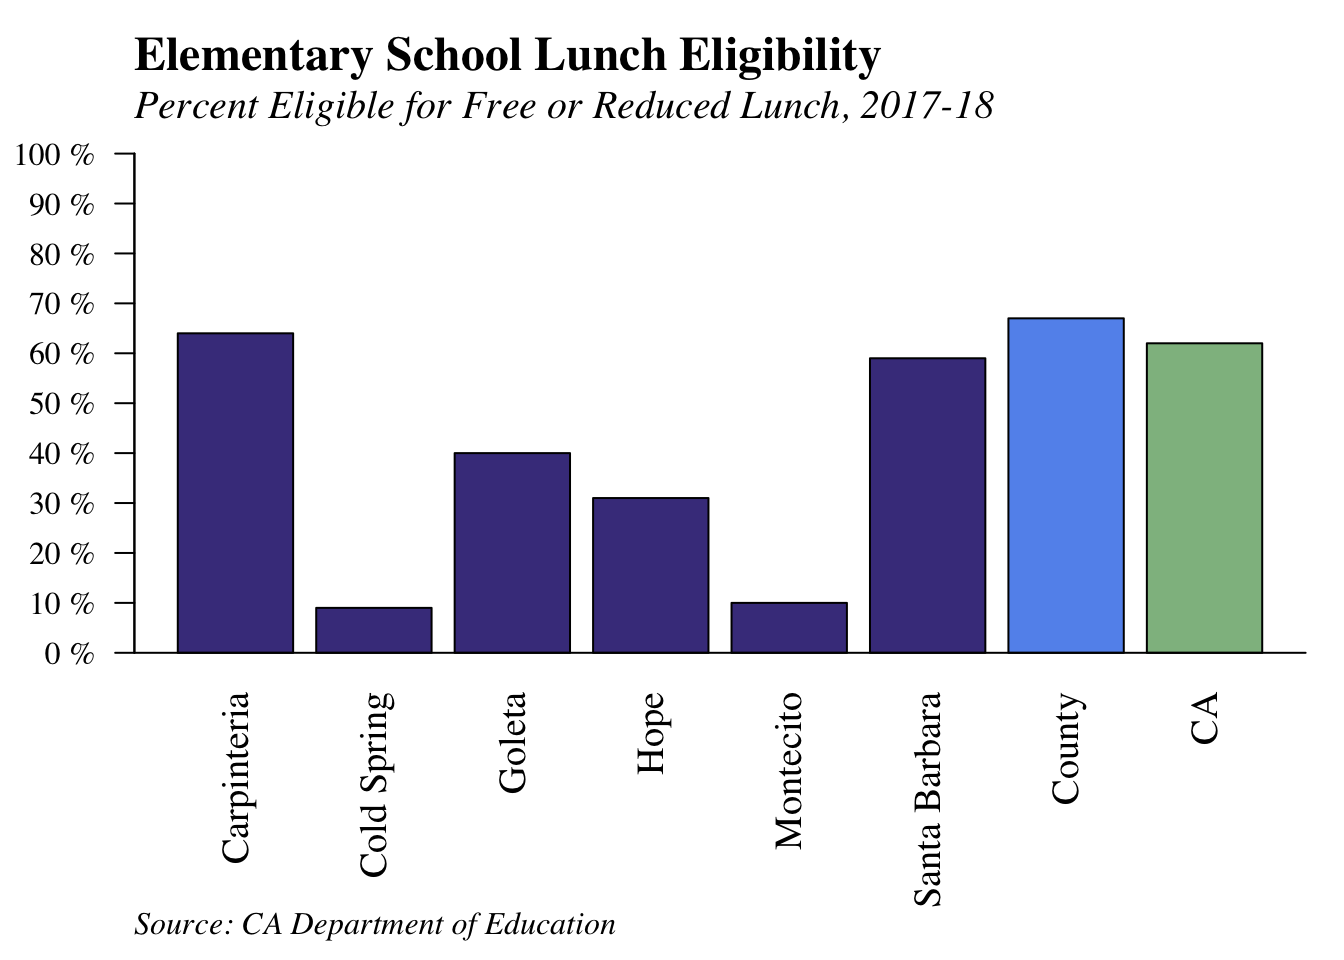
\includegraphics[width=0.95\linewidth]{cip_2019_files/figure-latex/unnamed-chunk-11-1}

\subsubsection*{What is the measure?}\label{what-is-the-measure-3}
\addcontentsline{toc}{subsubsection}{What is the measure?}

This statistic measures the number of calls to 911 in Santa Barbara
County in which domestic violence with a weapon is reported. Weapons
include guns, knives, heavy objects, hands, fists, and feet. This
specifically excludes verbal abuse.

\subsubsection*{How are we doing?}\label{how-are-we-doing-5}
\addcontentsline{toc}{subsubsection}{How are we doing?}

For the South Coast, weapon-related domestic violence calls to 911 have
fluctuated between a high of 365 in 2005 and a low of 28 in 2015 in the
last decade. In North County, the year 2005 represented the highest
number of incidents with 556 cases, and 2008 represented the lowest with
158. For the South Coast, the number of cases has remained fairly stable
since 2008, whereas North County saw a spike in weapon-related domestic
violence calls in 2009.

\subsection*{RAPE CRIME RATES INCREASE}\label{rape-crime-rates-increase}
\addcontentsline{toc}{subsection}{RAPE CRIME RATES INCREASE}

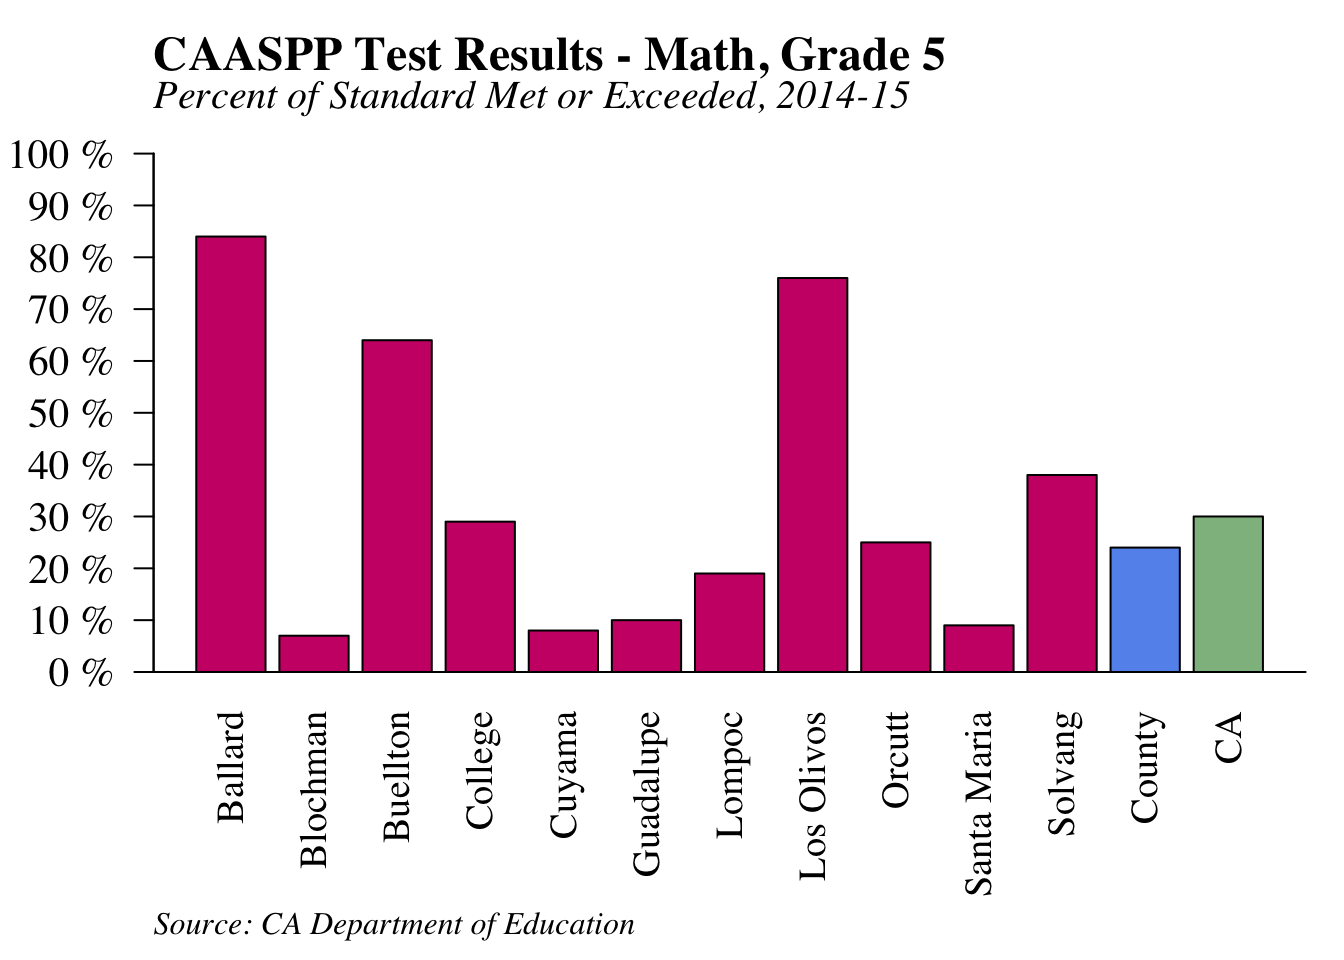
\includegraphics[width=0.95\linewidth]{cip_2019_files/figure-latex/unnamed-chunk-12-1}

\subsubsection*{What is the measure?}\label{what-is-the-measure-4}
\addcontentsline{toc}{subsubsection}{What is the measure?}

The number of reported rapes, calculated as the rate per 1,000 people.

\subsubsection*{Why is it important?}\label{why-is-it-important-3}
\addcontentsline{toc}{subsubsection}{Why is it important?}

Rape crimes play a very significant role in shaping the community's
sense of ``being safe.'' Because these crimes violate one's personal
rights, these crimes are both personally devastating and emotionally
tolling on a community.

\subsubsection*{How are we doing?}\label{how-are-we-doing-6}
\addcontentsline{toc}{subsubsection}{How are we doing?}

For the past several years, there has been a fair amount of variance in
the rape crime rate for both North County and the South Coast.
Currently, South Coast reached its highest rate at 0.52 incidents per
1,000 people compared to 0.33 incidents per 1,000 people in the prior
year. North County reached its highest rate in 2008, with 0.52 incidents
per 1,000 people. Currently, rates are down at 0.42 incidents per 1,000
people, a slight decrease from 2014.

\subsection*{BIRTHS TO TEENAGE MOTHERS
DECLINING}\label{births-to-teenage-mothers-declining}
\addcontentsline{toc}{subsection}{BIRTHS TO TEENAGE MOTHERS DECLINING}

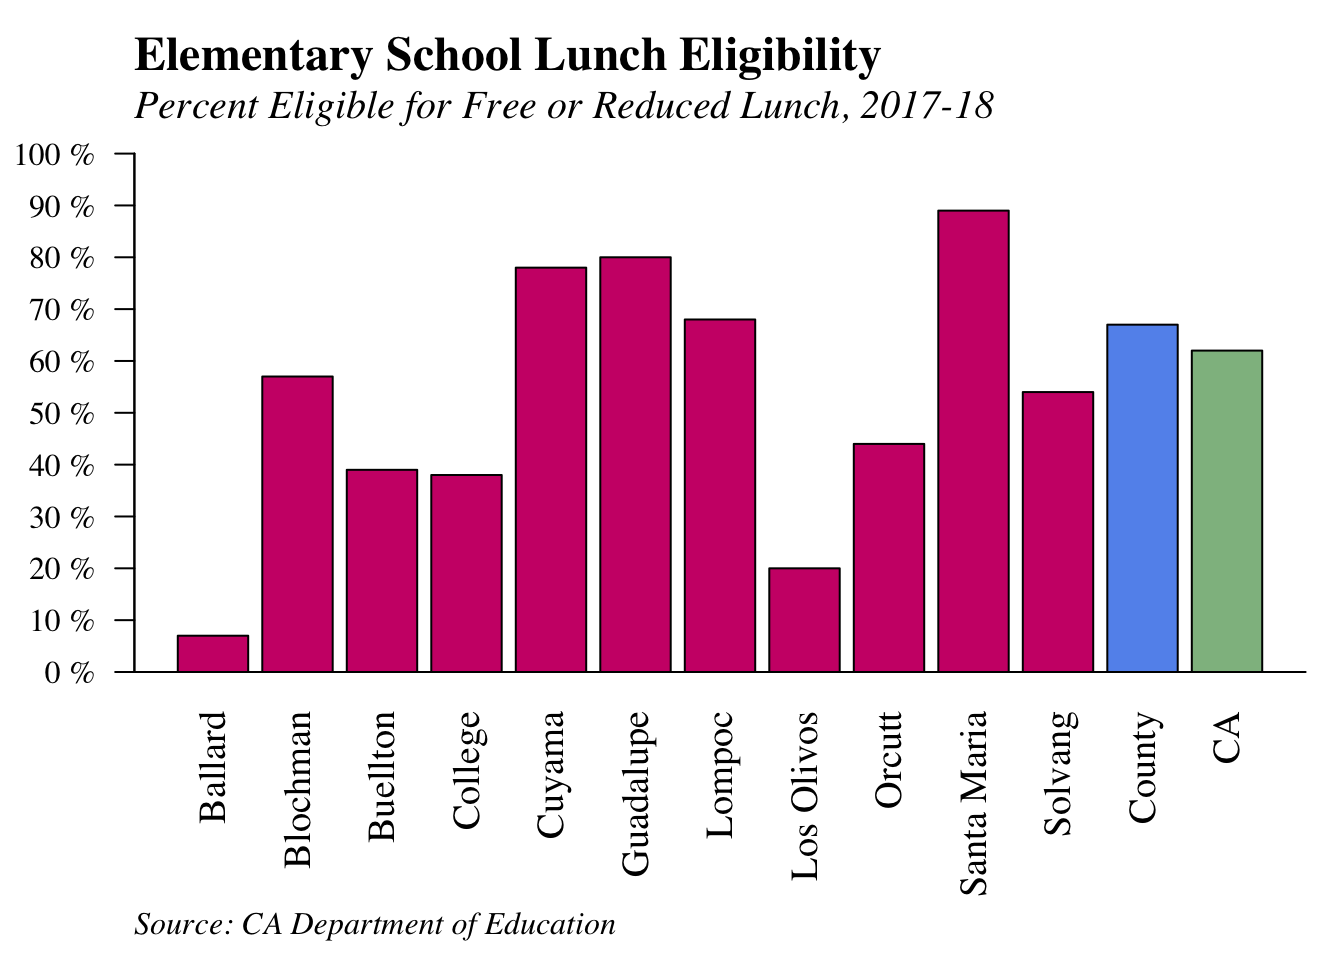
\includegraphics[width=0.95\linewidth]{cip_2019_files/figure-latex/unnamed-chunk-13-1}

\subsubsection*{What is the measure?}\label{what-is-the-measure-5}
\addcontentsline{toc}{subsubsection}{What is the measure?}

The number of children born to women between the ages of 15-19 as a
percentage of total births.

\subsubsection*{Why is it important?}\label{why-is-it-important-4}
\addcontentsline{toc}{subsubsection}{Why is it important?}

Births to teens represent a growing social concern. While children of
teenage mothers can be happy and healthy, they are at a higher risk of
suffering health problems than other children. Teenage mothers may face
great challenges in raising children because of the time conflicts with
attending school, lack of experience with child care, and the lack of
income necessary to provide for a child.

\subsubsection*{How are we doing?}\label{how-are-we-doing-7}
\addcontentsline{toc}{subsubsection}{How are we doing?}

The percentage of teen births in the Santa Barbara County reached its
lowest point in 2014, reaching a rate of only 23 births per 1,000 teens.

\subsection*{MOTHERS RECEIVING INADEQUATE PRENATAL CARE
DROPS}\label{mothers-receiving-inadequate-prenatal-care-drops}
\addcontentsline{toc}{subsection}{MOTHERS RECEIVING INADEQUATE PRENATAL
CARE DROPS}

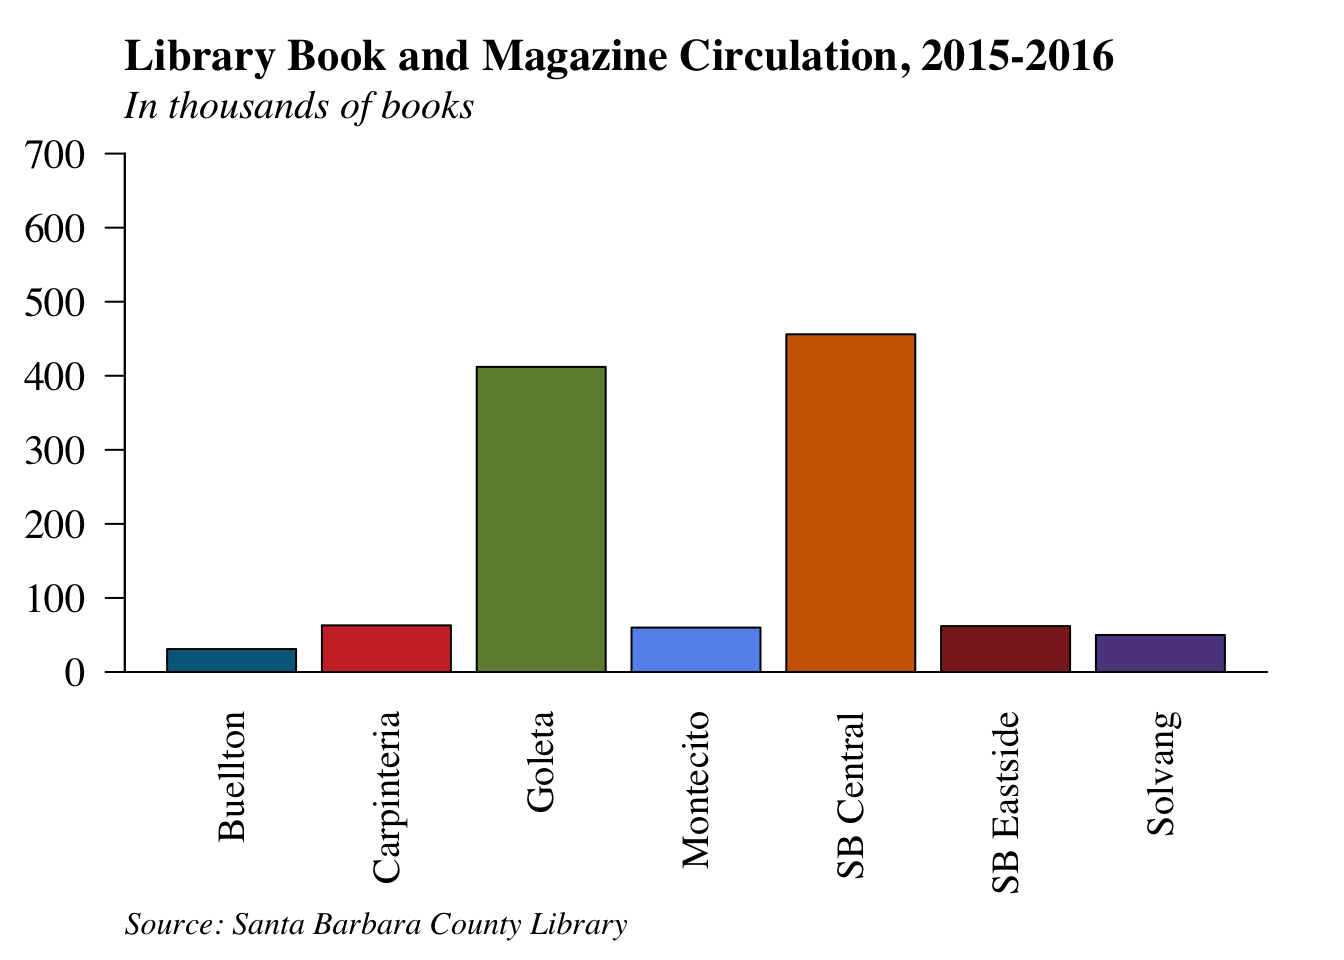
\includegraphics[width=0.95\linewidth]{cip_2019_files/figure-latex/unnamed-chunk-14-1}

\subsubsection*{What is the measure?}\label{what-is-the-measure-6}
\addcontentsline{toc}{subsubsection}{What is the measure?}

The percentage of total births in the Santa Barbara County in which the
mother does not receive any prenatal care within the first three months
of pregnancy.

\subsubsection*{Why is it important?}\label{why-is-it-important-5}
\addcontentsline{toc}{subsubsection}{Why is it important?}

The level of prenatal care is not only a leading indicator of successful
pregnancies, but also a predictor of a child's health later in life.

\subsubsection*{How are we doing?}\label{how-are-we-doing-8}
\addcontentsline{toc}{subsubsection}{How are we doing?}

In the past ten years, inadequate prenatal care has fluctuated reaching
a peak of 28.4 percent in 2009. However, the percentage of mothers
receiving inadequate prenatal care has decreased since then, hovering
around 23.2 percent. In 2014, it dropped to 22.3 percent.

\subsection*{INFANT MORTALITY RATES SPIKE IN
2014}\label{infant-mortality-rates-spike-in-2014}
\addcontentsline{toc}{subsection}{INFANT MORTALITY RATES SPIKE IN 2014}

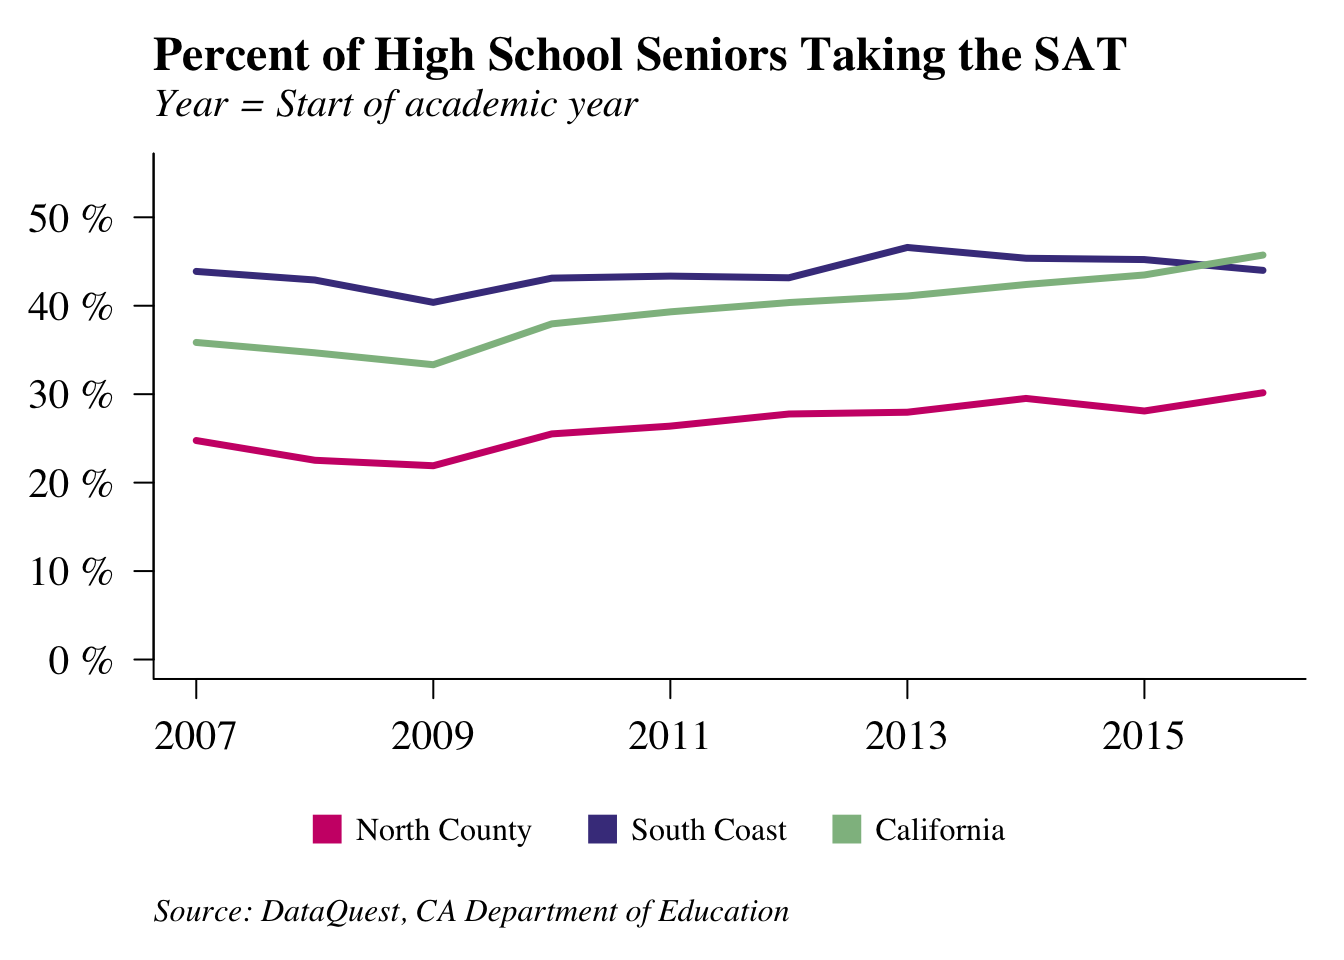
\includegraphics[width=0.95\linewidth]{cip_2019_files/figure-latex/unnamed-chunk-15-1}

\subsubsection*{What is the measure?}\label{what-is-the-measure-7}
\addcontentsline{toc}{subsubsection}{What is the measure?}

The number of deaths of infants one year and under per 1,000 live births
in Santa Barbara County.

\subsubsection*{Why is it important?}\label{why-is-it-important-6}
\addcontentsline{toc}{subsubsection}{Why is it important?}

In addition to the emotional damage caused to parents, high infant
mortality rates are often an indication of a mother's poor health or of
inadequate healthcare and services. Infant mortality is often attributed
to congenital abnormalities, low birthweight, Sudden Infant Death
Syndrome (SIDS), or problems related to complications of pregnancies.

\subsubsection*{How are we doing?}\label{how-are-we-doing-9}
\addcontentsline{toc}{subsubsection}{How are we doing?}

Infant mortality rates decreased sharply from 2011 to 2012, falling from
4.8 to 2.9 deaths per 1,000 live births. The rate in 2013 remained
stable at 2.8 deaths per 1,000 live births, decreasing only slightly
from 2012's rate. However, 2014 saw a marked increase in the infant
mortality rate, which spiked to 3.3. Still, this rate remains lower than
most years in the past.

\subsection*{ELEMENTARY SCHOOL LUNCH PARTICIPATION INCREASES IN NORTH
COUNTY}\label{elementary-school-lunch-participation-increases-in-north-county}
\addcontentsline{toc}{subsection}{ELEMENTARY SCHOOL LUNCH PARTICIPATION
INCREASES IN NORTH COUNTY}

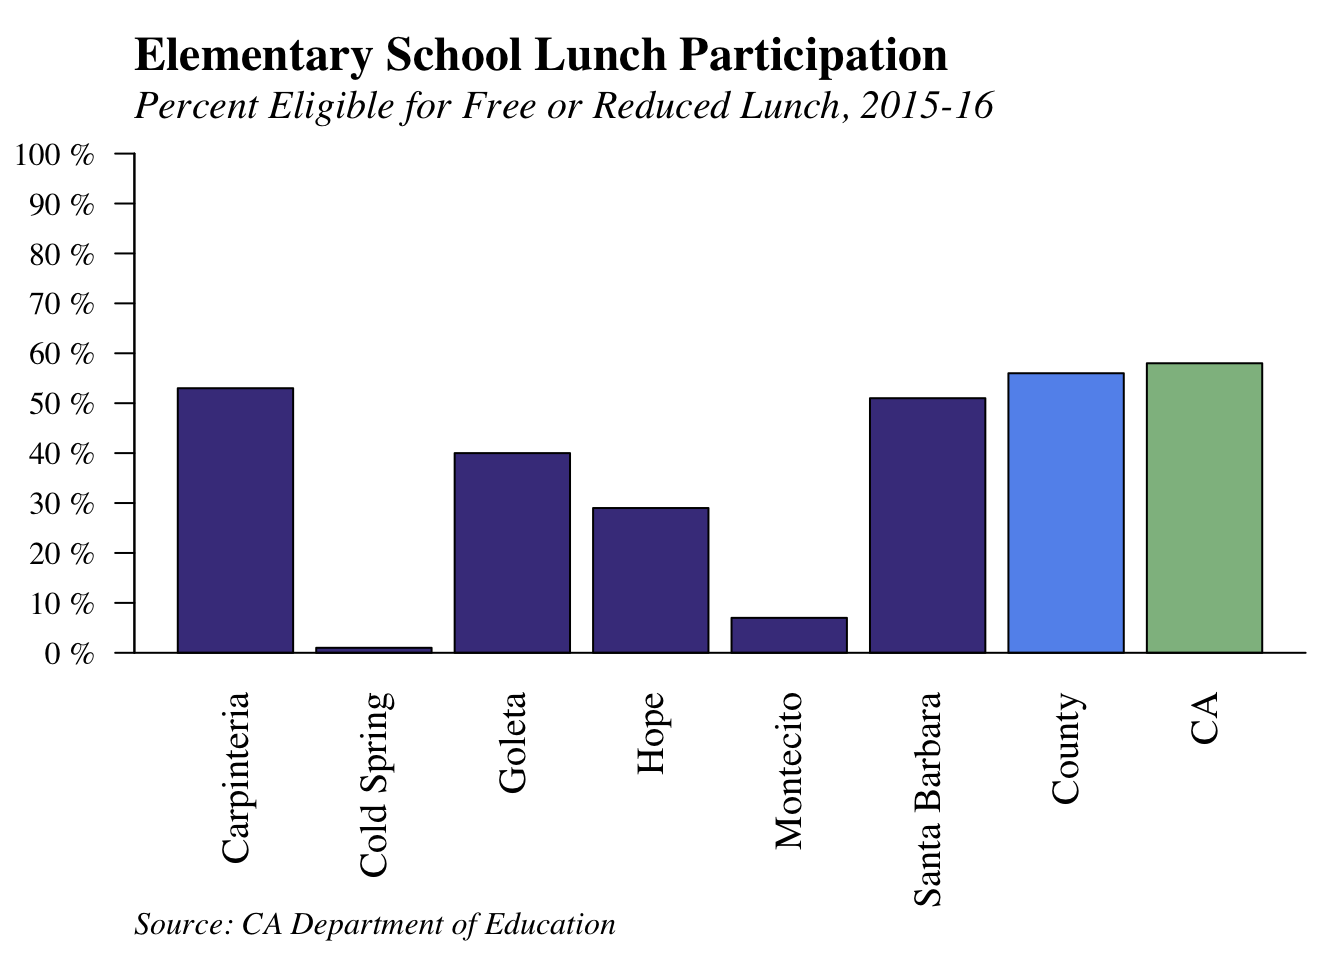
\includegraphics[width=0.95\linewidth]{cip_2019_files/figure-latex/unnamed-chunk-16-1}

\subsubsection*{What is the measure?}\label{what-is-the-measure-8}
\addcontentsline{toc}{subsubsection}{What is the measure?}

This program provides federally sponsored, free, or subsidized school
lunch programs in local public elementary schools. Because families must
demonstrate financial need in order to participate, this measure
reflects the percentage of children living in families with low incomes.

\subsubsection*{Why is it important?}\label{why-is-it-important-7}
\addcontentsline{toc}{subsubsection}{Why is it important?}

In many ways, children are the most sensitive to any negative forces in
our families and communities. While it is true that many children from
poorer families benefit from a solid family structure and do very well
in society, financial strain is often seen as having a negative impact
on a child's opportunities. At a minimum, children from poorer families
often have diminished access to education and health care.

\subsubsection*{How are we doing?}\label{how-are-we-doing-10}
\addcontentsline{toc}{subsubsection}{How are we doing?}

While school lunch participation generally increased throughout the late
2000s to early 2010s, recently the percentage of students eligible for
the program has stagnated across the South Coast. When comparing the
South Coast to North County and statewide levels, the South Coast has
less participation in these programs. North County, however, has
slightly more eligible students than the statewide average. This number
has increased in the last year. It is important to note that eligibility
also varies within North County, with some school districts seeing much
less eligibility than others.

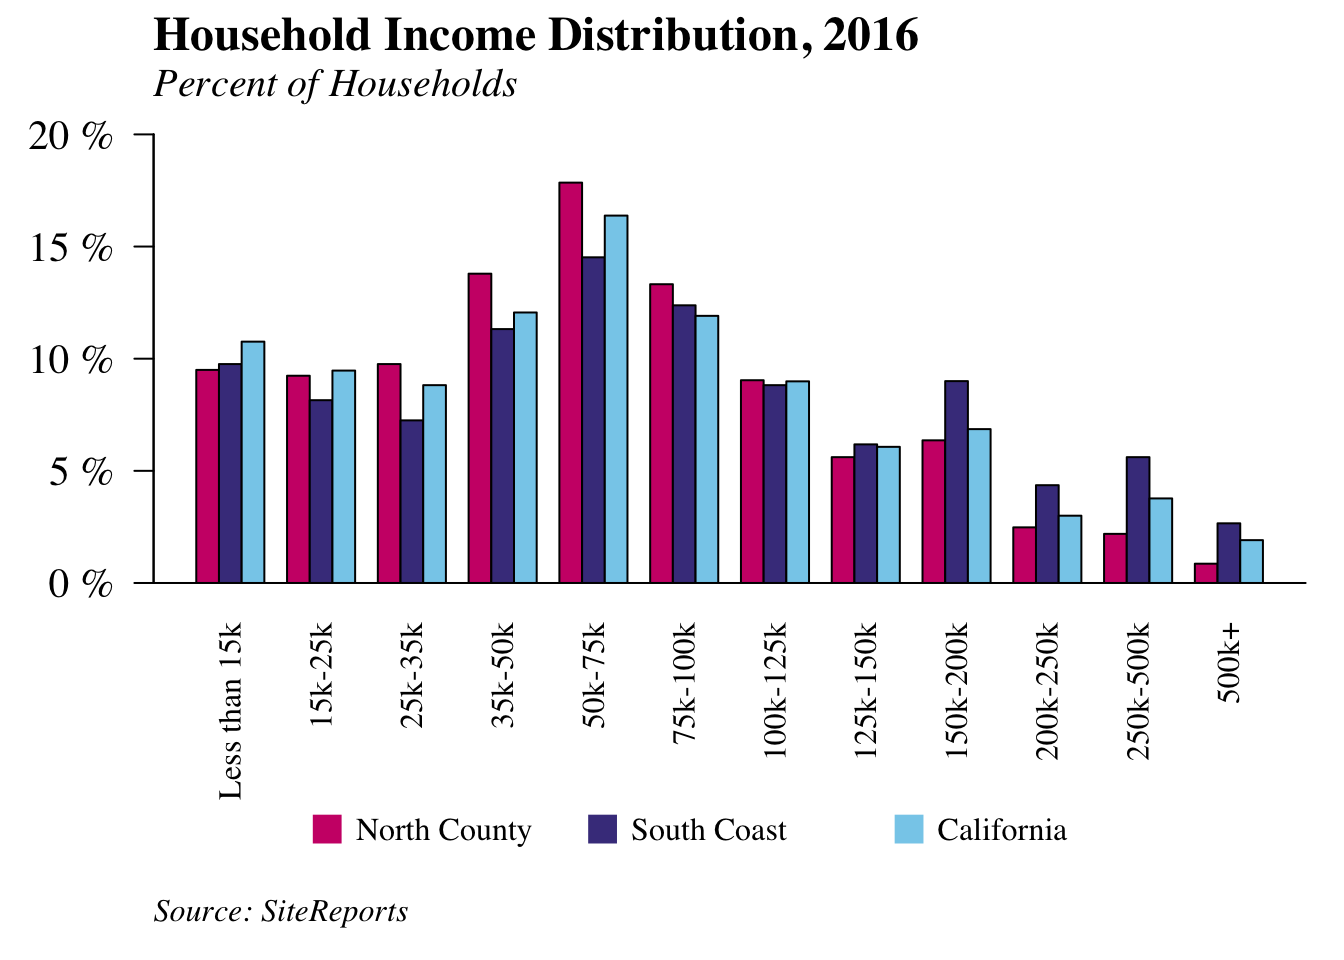
\includegraphics[width=0.95\linewidth]{cip_2019_files/figure-latex/unnamed-chunk-17-1}

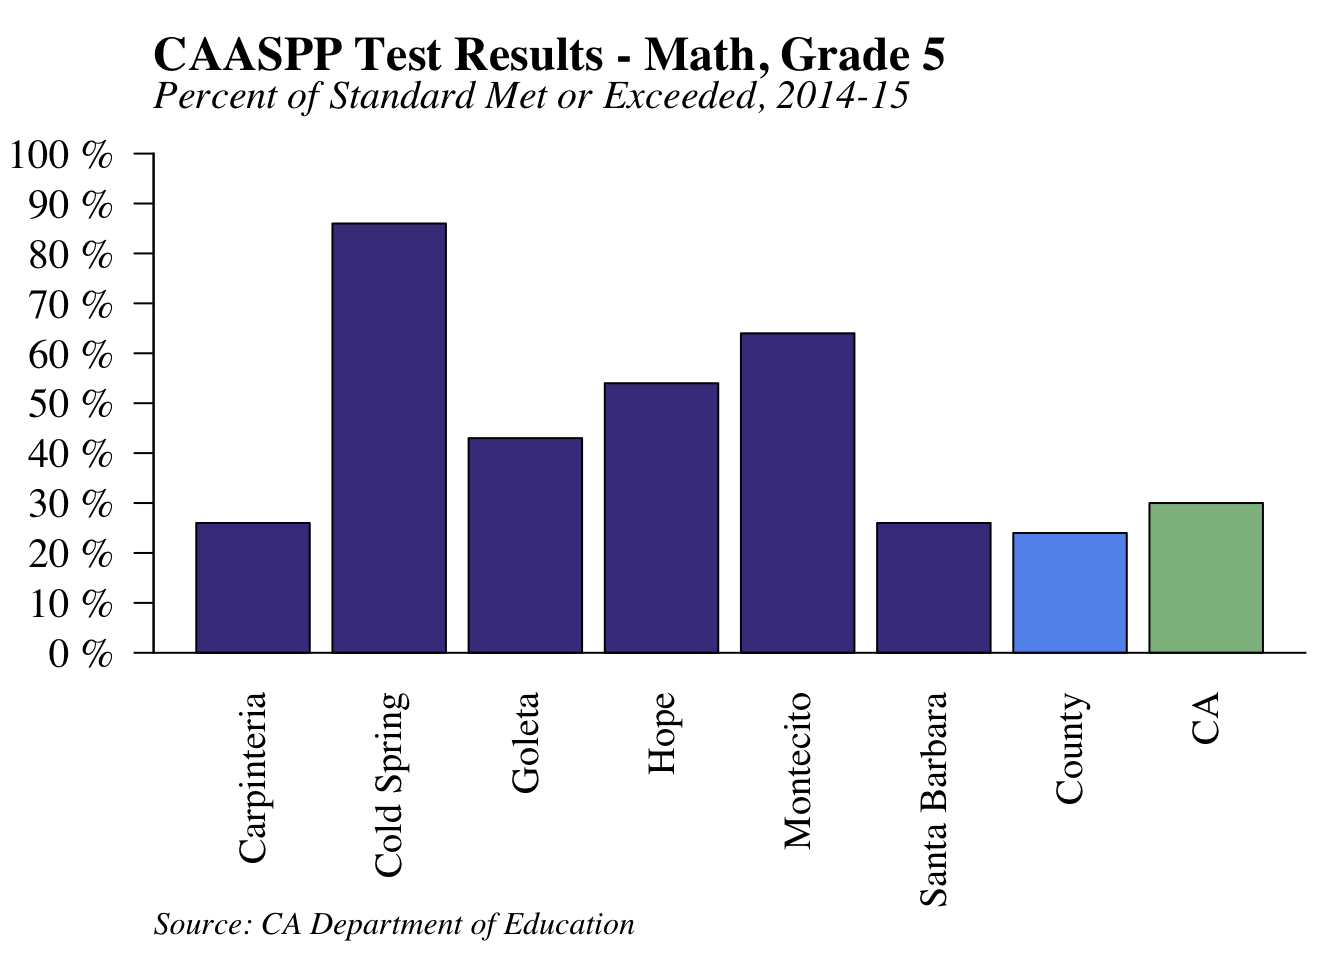
\includegraphics[width=0.95\linewidth]{cip_2019_files/figure-latex/unnamed-chunk-18-1}

\section*{Poverty in the County}\label{poverty-in-the-county}
\addcontentsline{toc}{section}{Poverty in the County}

\subsection*{HOUSEHOLD INCOME
DISTRIBUTION}\label{household-income-distribution}
\addcontentsline{toc}{subsection}{HOUSEHOLD INCOME DISTRIBUTION}

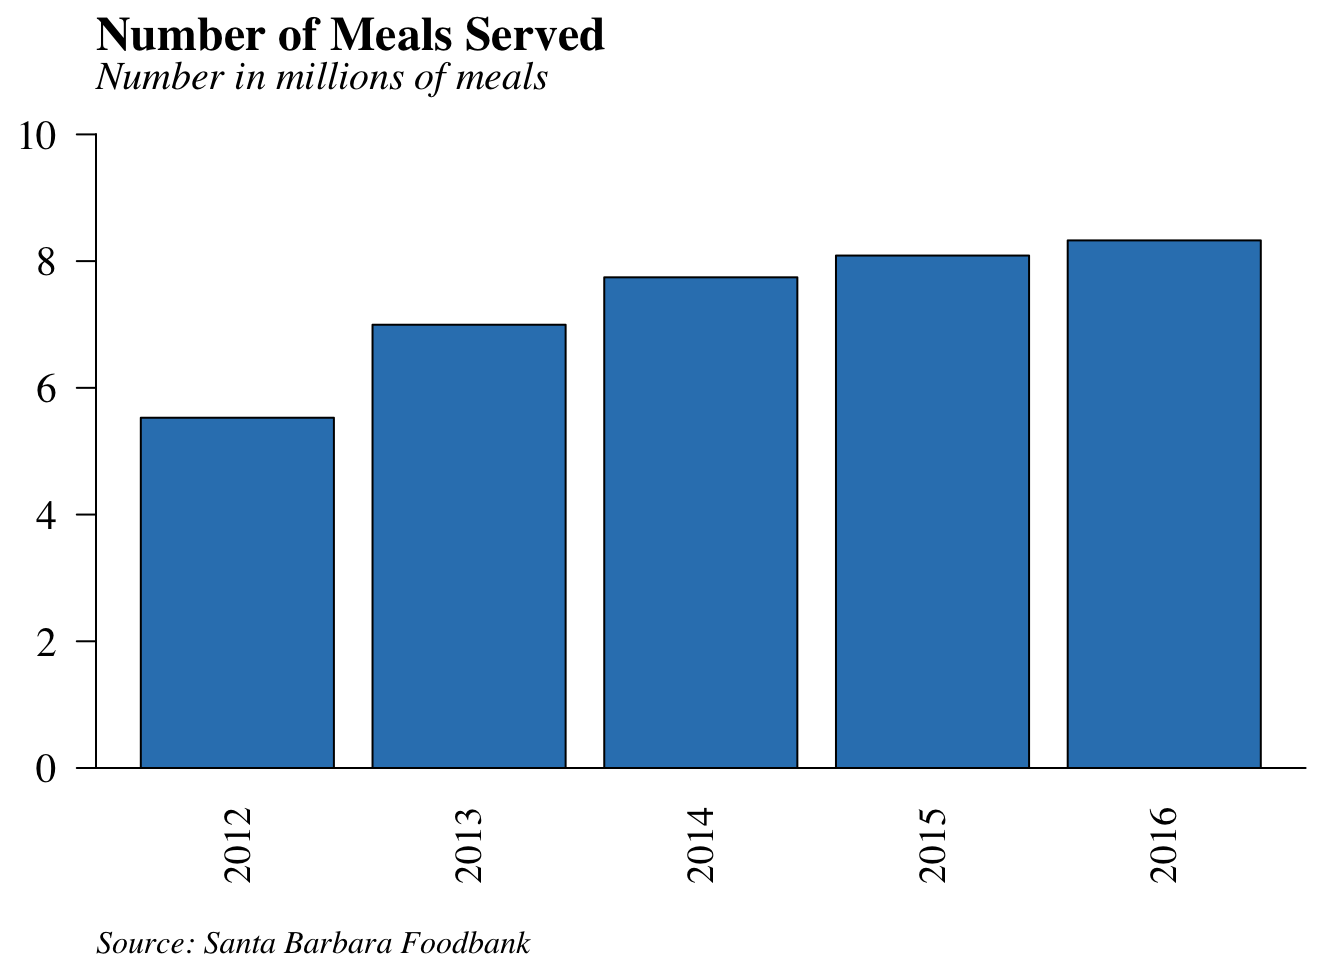
\includegraphics[width=0.95\linewidth]{cip_2019_files/figure-latex/unnamed-chunk-19-1}

\subsubsection*{What is the measure?}\label{what-is-the-measure-9}
\addcontentsline{toc}{subsubsection}{What is the measure?}

The percent of households falling in certain income ranges for North
County, the South Coast, and California in 2016.

\subsubsection*{Why is it important?}\label{why-is-it-important-8}
\addcontentsline{toc}{subsubsection}{Why is it important?}

The overall health of a community depends on the ability of its
residents to afford basic needs such as food, clothing, shelter, and
medical care. The income distribution breaks down the earnings and
allows us to examine the percent of families that can afford a certain
quality of life. We can use the income distribution to draw an overview
of the economic composition of the community and how it compares to
California.

\subsubsection*{How are we doing?}\label{how-are-we-doing-11}
\addcontentsline{toc}{subsubsection}{How are we doing?}

The South Coast tends to be wealthier than North County and California,
with higher percentages of its residents falling at the upper end of the
income distribution range. California also has a larger percentage of
households making less than \$15,000 a year than North County and the
South Coast.

\subsection*{POVERTY STATUS OF
FAMILIES}\label{poverty-status-of-families}
\addcontentsline{toc}{subsection}{POVERTY STATUS OF FAMILIES}

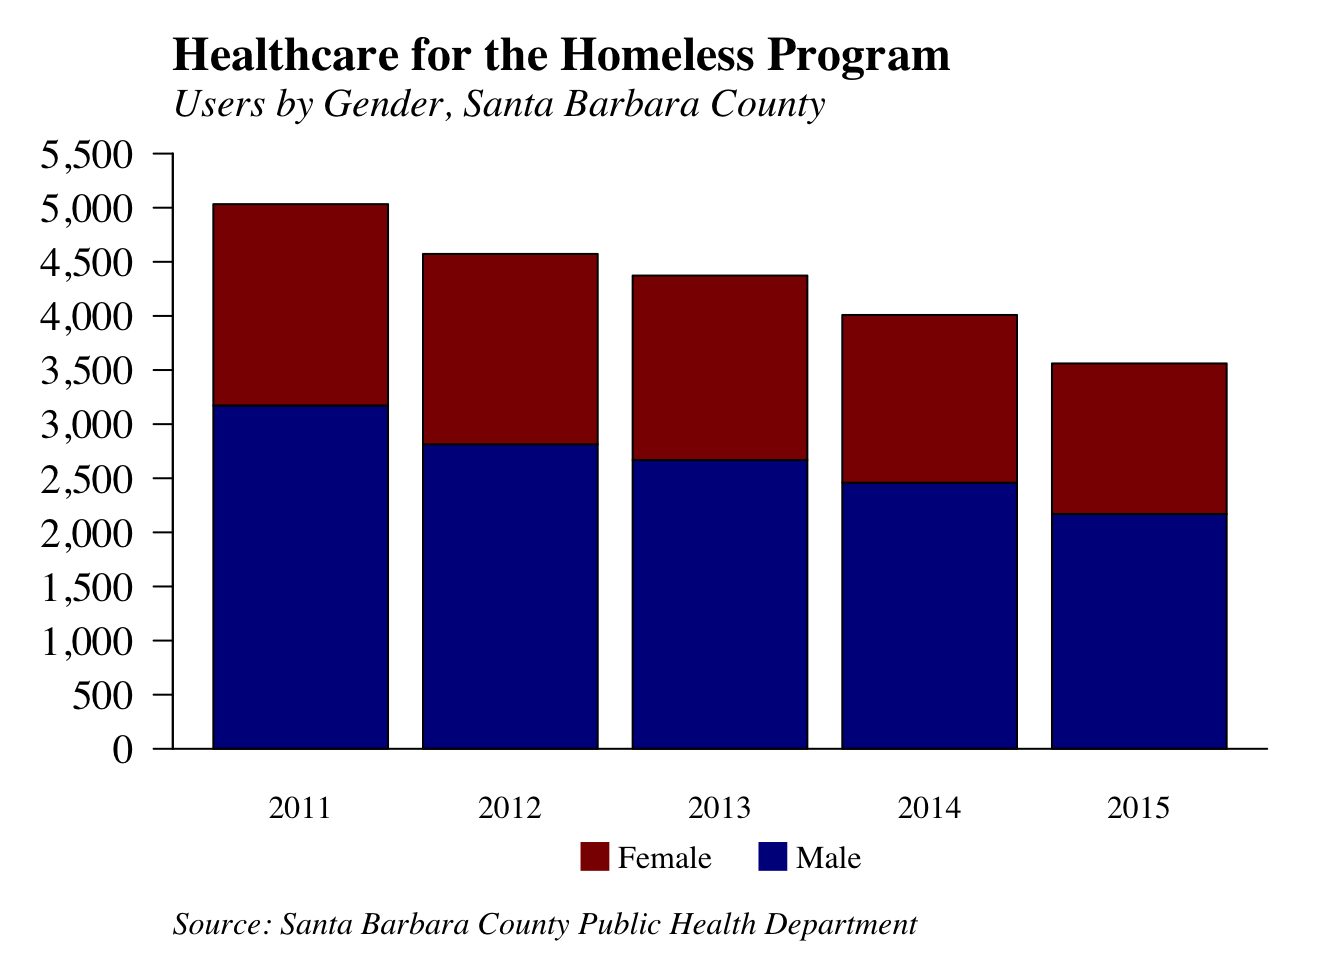
\includegraphics[width=0.95\linewidth]{cip_2019_files/figure-latex/unnamed-chunk-20-1}

\subsubsection*{What is the measure?}\label{what-is-the-measure-10}
\addcontentsline{toc}{subsubsection}{What is the measure?}

A breakdown of the composition of families with incomes at, above, and
below poverty in Santa Barbara County.

\subsubsection*{Why is it important?}\label{why-is-it-important-9}
\addcontentsline{toc}{subsubsection}{Why is it important?}

Understanding the composition of families living in poverty allows us to
see which part of the population is suffering the most from poor wages.

\subsubsection*{How are we doing?}\label{how-are-we-doing-12}
\addcontentsline{toc}{subsubsection}{How are we doing?}

Most families with incomes below the Federal Poverty Level are families
with children. 83 percent of the 6,714 households living in poverty in
North County are families with children. 77 percent of the 2,081
households living in poverty in South Coast are families with children.
This indicates that many children in the Santa Barbara County may be
going without some of the basic needs that are crucial in children's
early development.

\subsection*{NUMBERS OF MEALS SERVED INCREASES, 35 PERCENT OF THOSE
SERVED ARE UNDER
18}\label{numbers-of-meals-served-increases-35-percent-of-those-served-are-under-18}
\addcontentsline{toc}{subsection}{NUMBERS OF MEALS SERVED INCREASES, 35
PERCENT OF THOSE SERVED ARE UNDER 18}

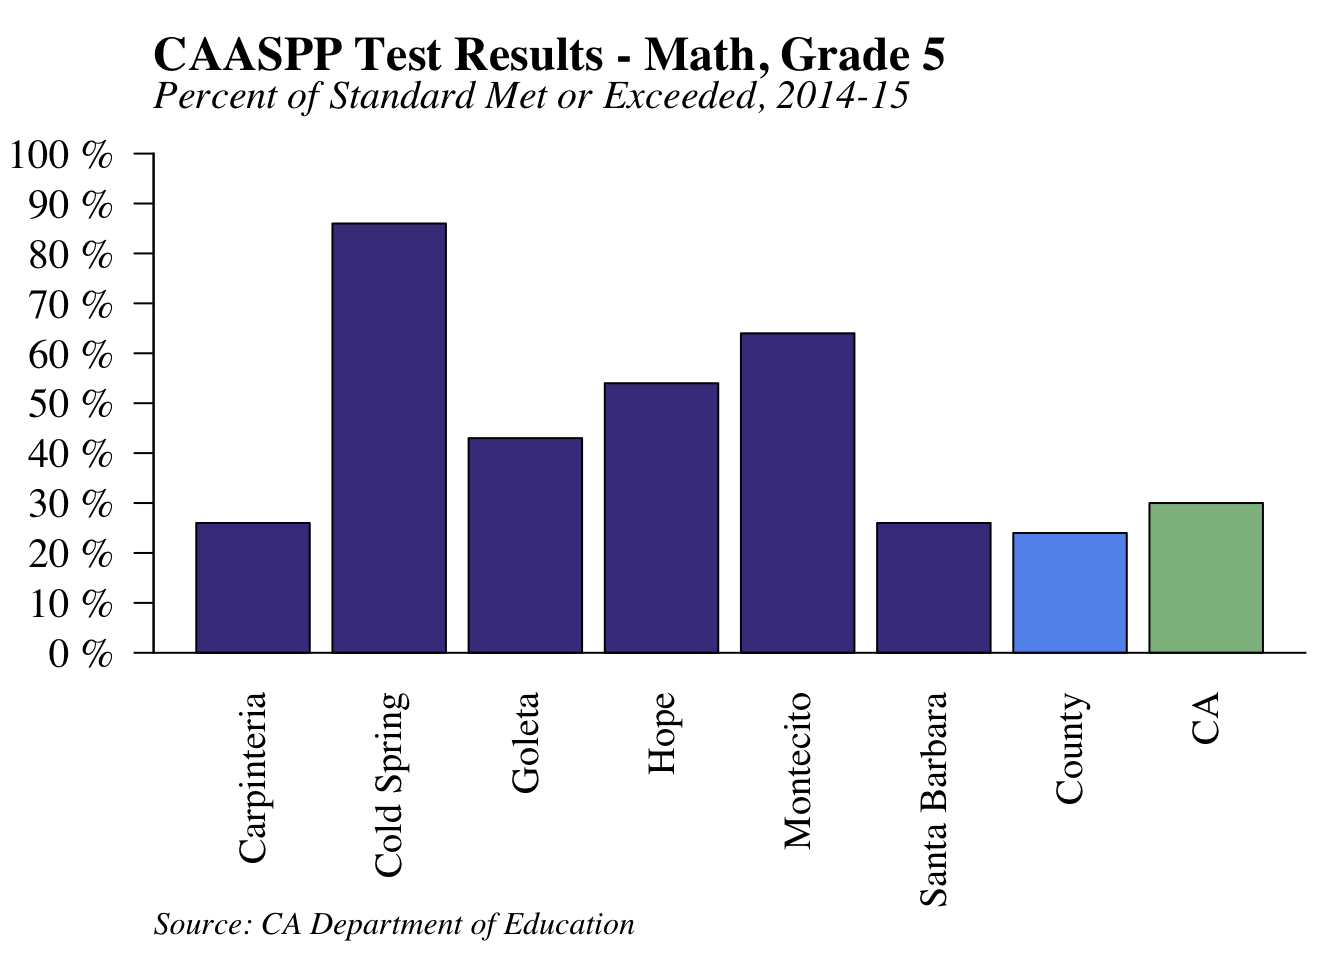
\includegraphics[width=0.95\linewidth]{cip_2019_files/figure-latex/unnamed-chunk-21-1}
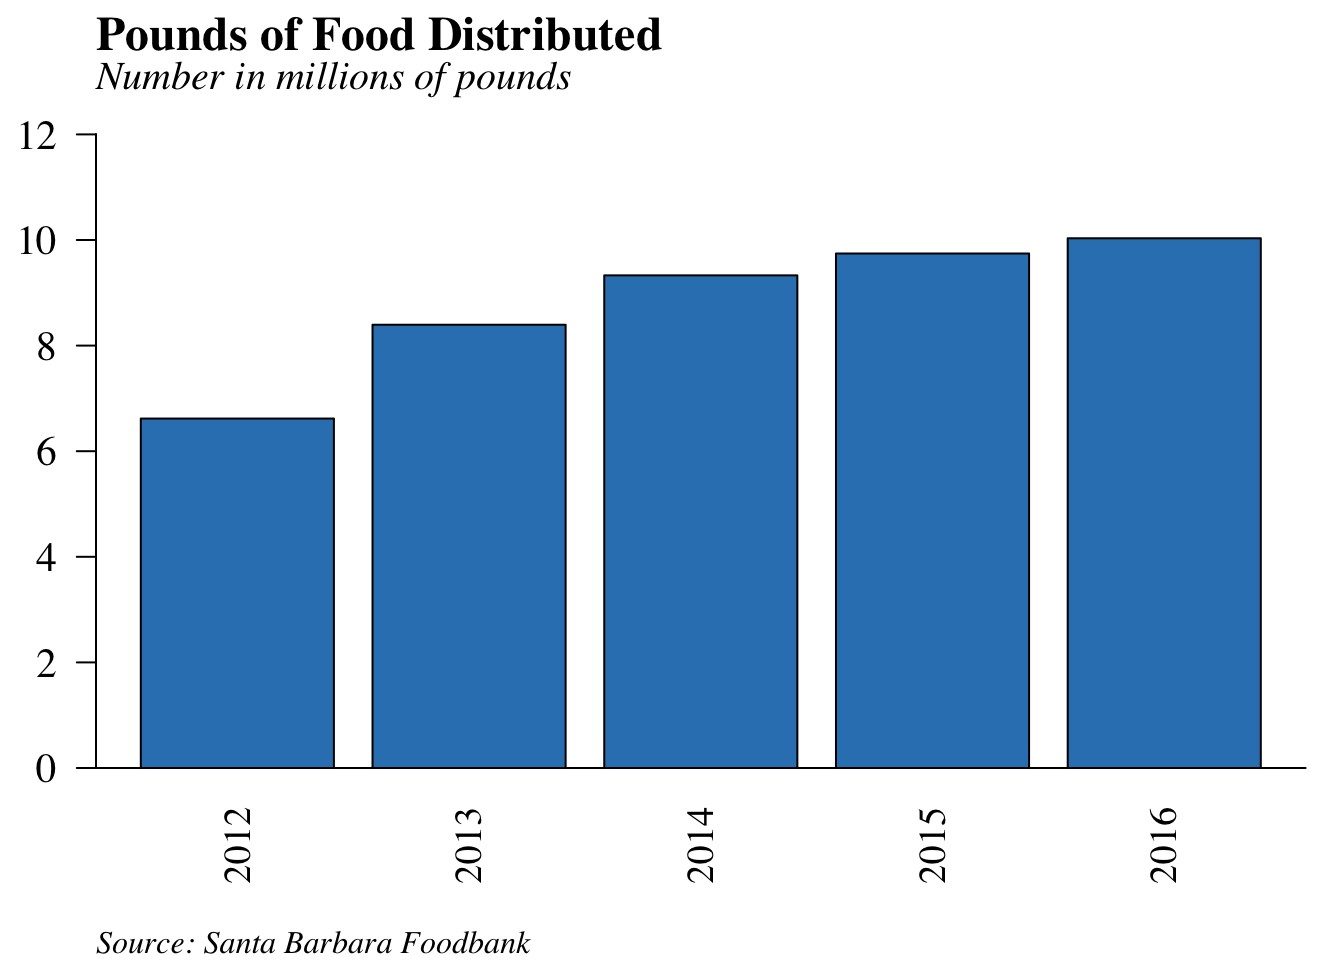
\includegraphics[width=0.95\linewidth]{cip_2019_files/figure-latex/unnamed-chunk-21-2}
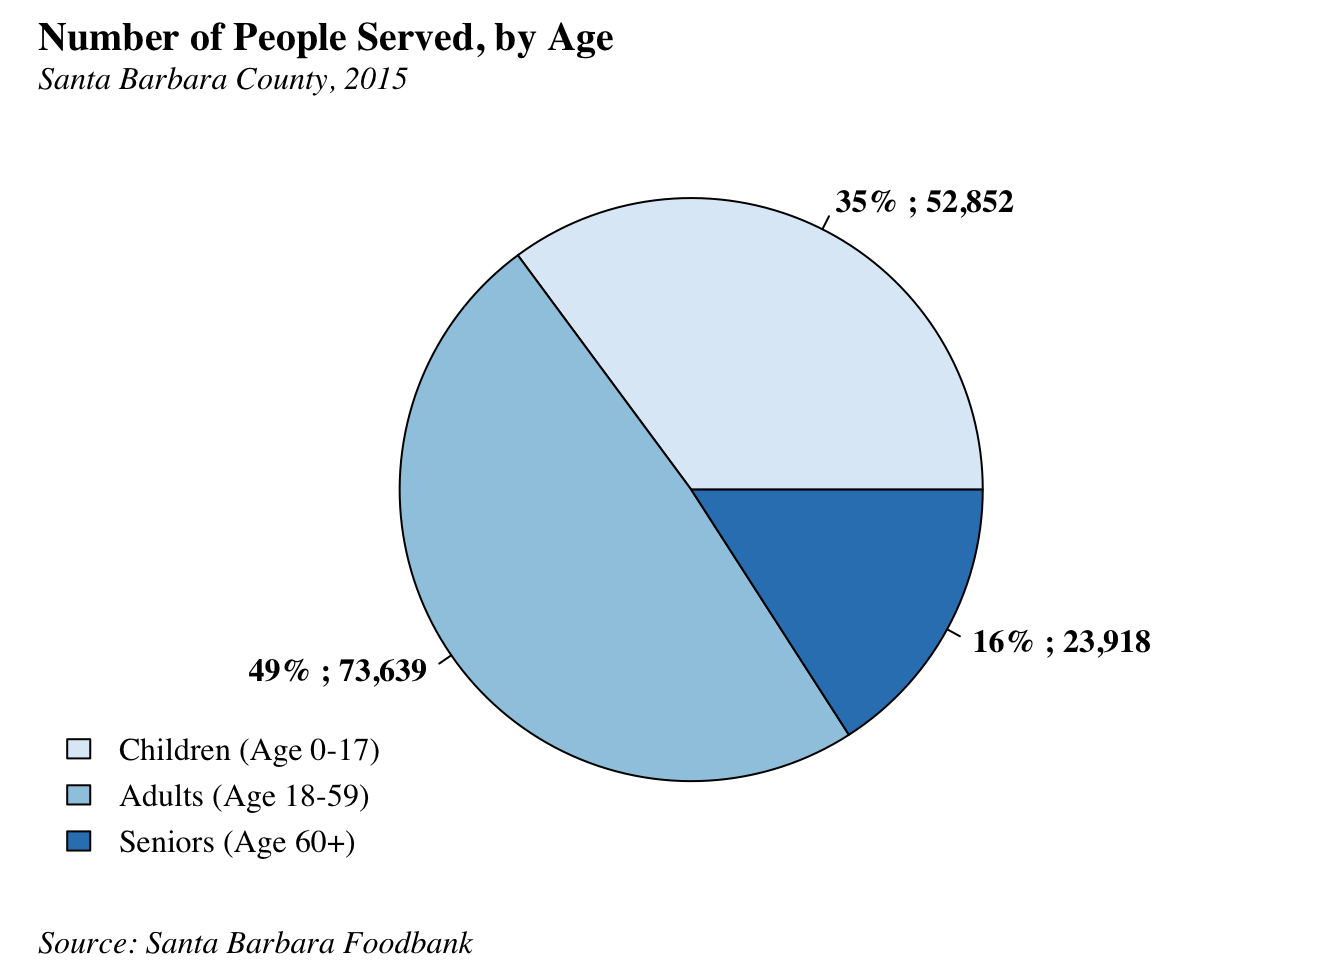
\includegraphics[width=0.95\linewidth]{cip_2019_files/figure-latex/unnamed-chunk-21-3}

\subsubsection*{What is the measure?}\label{what-is-the-measure-11}
\addcontentsline{toc}{subsubsection}{What is the measure?}

The amount of food distributed by Santa Barbara County Foodbank, the
number of people served in Santa Barbara County food kitchens, and the
age of those served in 2016.

\subsubsection*{Why are they important?}\label{why-are-they-important-1}
\addcontentsline{toc}{subsubsection}{Why are they important?}

People use food kitchens when they cannot afford to buy enough food for
themselves or their families, and good nutrition is an essential part of
staying healthy. The number of people using food banks is often
indicative of the number of people living at or below the poverty level
within a community.

\subsubsection*{How are we doing?}\label{how-are-we-doing-13}
\addcontentsline{toc}{subsubsection}{How are we doing?}

The pounds of food distributed and number of meals served in Santa
Barbara County increased by 3 percent from 2014 to 2015, whereas the
number of people served also increased by 3 percent from 146,198 to
150,409 people. This indicates that food contributions are rising at the
same pace as the amount of people needing to be fed. Of the 150,409
people served in Santa Barbara County, 35 percent of them were under the
age of 18. A considerable number of young people in Santa Barbara County
live in families that do not earn enough money to provide adequate
nutrition for their children.

\subsection*{NUMBER OF HOMELESS USING HEALTH CARE PROGRAM FOLLOWS
DECREASING
TREND}\label{number-of-homeless-using-health-care-program-follows-decreasing-trend}
\addcontentsline{toc}{subsection}{NUMBER OF HOMELESS USING HEALTH CARE
PROGRAM FOLLOWS DECREASING TREND}

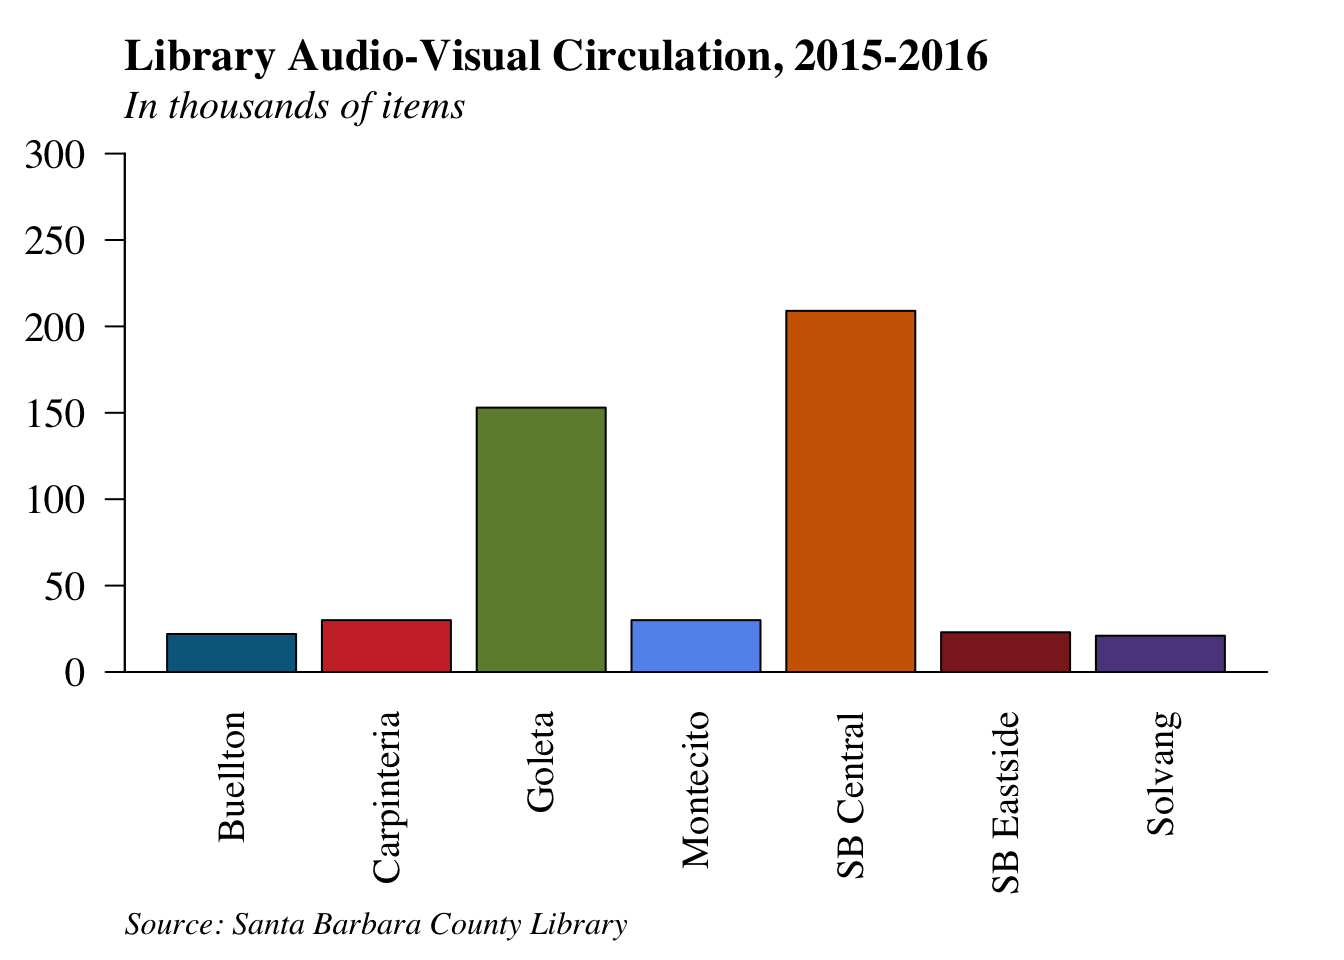
\includegraphics[width=0.95\linewidth]{cip_2019_files/figure-latex/unnamed-chunk-22-1}

\subsubsection*{What is the measure?}\label{what-is-the-measure-12}
\addcontentsline{toc}{subsubsection}{What is the measure?}

The number of users of the Health Care for the Homeless program broken
down by gender. The Health Care for the Homeless program is federally
funded and allows homeless people to receive medical attention.

\subsubsection*{Why is it important?}\label{why-is-it-important-10}
\addcontentsline{toc}{subsubsection}{Why is it important?}

The overall health of a community depends on the physical and mental
health of all of its members. Providing health care for the homeless
permits more people in the community to remain in good health.

\subsubsection*{How are we doing?}\label{how-are-we-doing-14}
\addcontentsline{toc}{subsubsection}{How are we doing?}

The number of homeless people using the program has continued its
downward trend since 2011. In 2015, 2,170 men and 1,391 women utilized
this federal program, compared to 3,173 men and 1860 women in 2011.
Given the challenges of attempting to measure the homeless and transient
population, it is difficult to determine if these decreases reflect a
smaller number of homeless people taking advantage of the program, or a
decrease in the homeless population being served.

\subsection*{OVER 15 PERCENT OF COUNTY JOBS PAY LESS THAN POVERTY
GUIDELINES}\label{over-15-percent-of-county-jobs-pay-less-than-poverty-guidelines}
\addcontentsline{toc}{subsection}{OVER 15 PERCENT OF COUNTY JOBS PAY
LESS THAN POVERTY GUIDELINES}

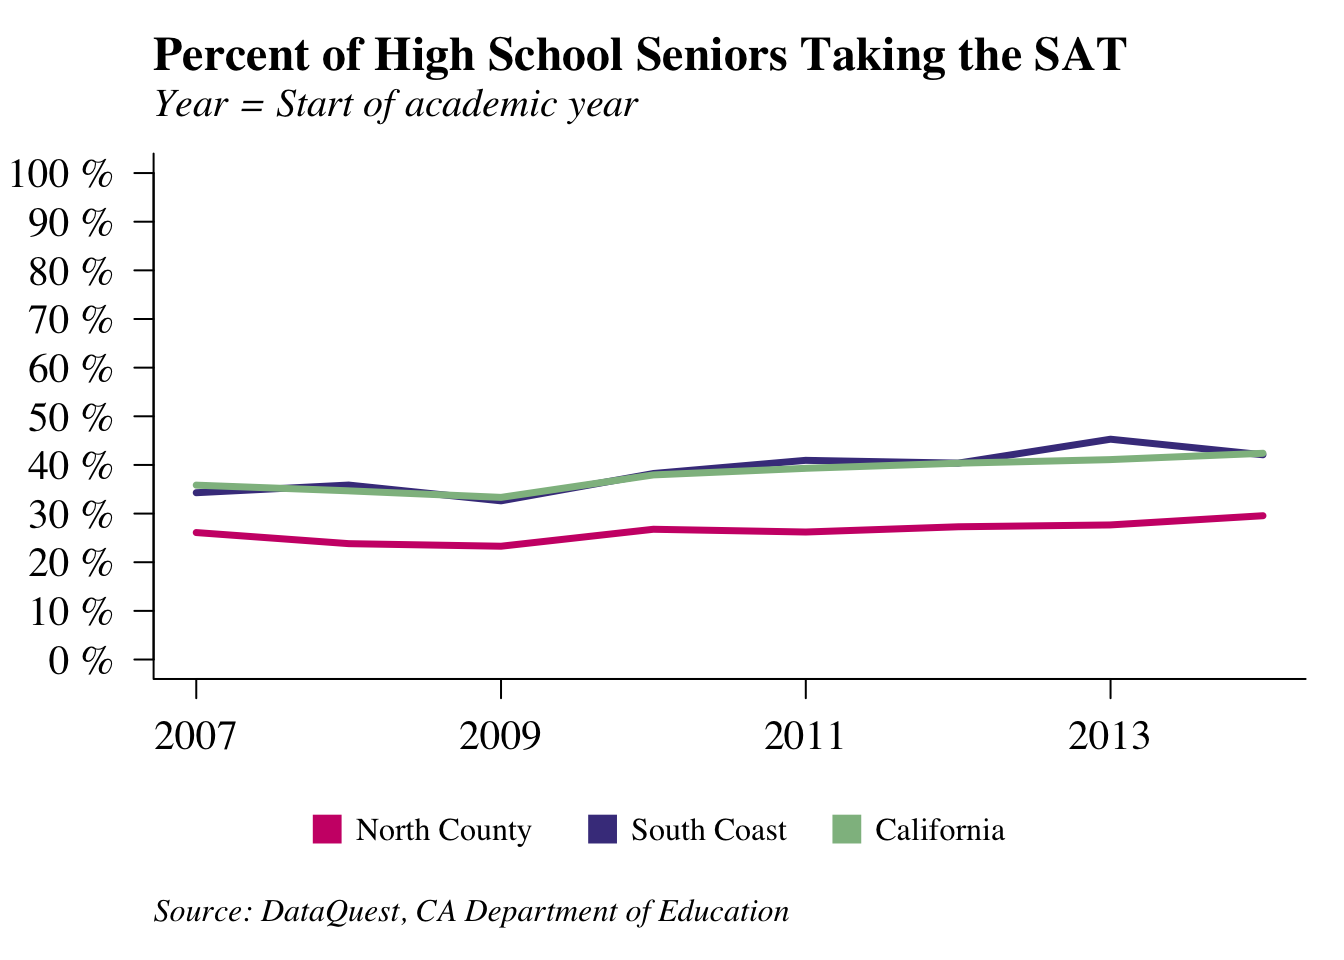
\includegraphics[width=0.95\linewidth]{cip_2019_files/figure-latex/unnamed-chunk-23-1}

\subsubsection*{What is the measure?}\label{what-is-the-measure-13}
\addcontentsline{toc}{subsubsection}{What is the measure?}

The percentage of jobs in Santa Barbara County that pay below or above
the poverty guidelines. For a household of three, the poverty guideline
in 2016 is \$20,160 or \$10.08 per hour, which assumes 2000 working
hours per year.

\subsubsection*{Why is it important?}\label{why-is-it-important-11}
\addcontentsline{toc}{subsubsection}{Why is it important?}

Positions that pay less than the Federal Poverty guideline denies people
the ability to afford their needs and detracts from their quality of
life.

\subsubsection*{How are we doing?}\label{how-are-we-doing-15}
\addcontentsline{toc}{subsubsection}{How are we doing?}

15 percent of all jobs pay less than the Federal Poverty guideline, and
over 22 percent pay over 200 percent of the guideline. Therefore,
approximately one job in six fall below the Federal Poverty guideline,
while over one in five pay 200 percent above the Federal Poverty
guideline in Santa Barbara County.

\section*{Education}\label{education}
\addcontentsline{toc}{section}{Education}

\subsection*{SAT SCORES CONTINUE DOWNWARD
TREND}\label{sat-scores-continue-downward-trend}
\addcontentsline{toc}{subsection}{SAT SCORES CONTINUE DOWNWARD TREND}

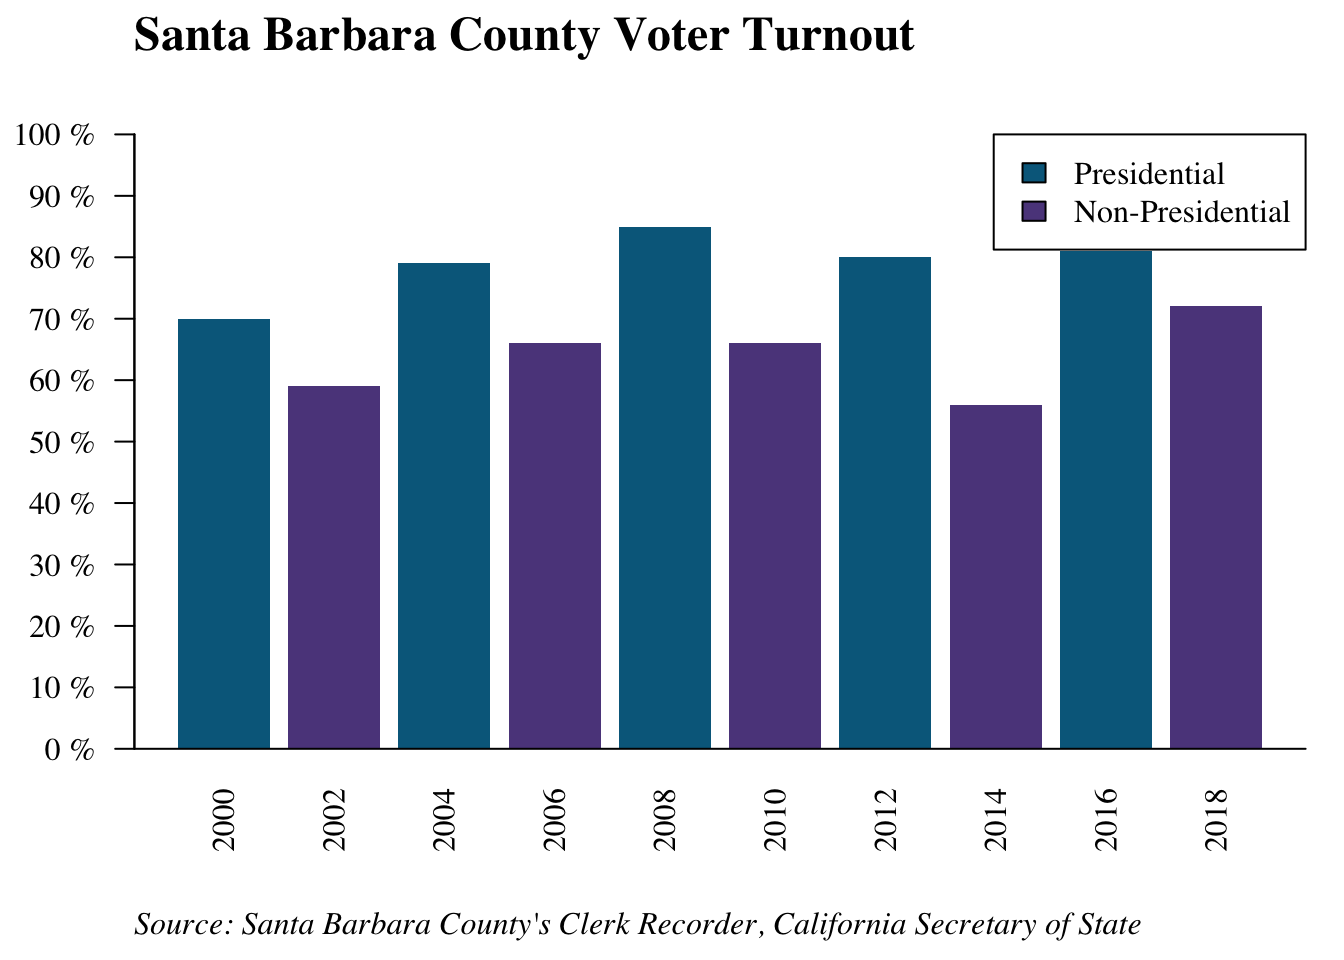
\includegraphics[width=0.95\linewidth]{cip_2019_files/figure-latex/unnamed-chunk-24-1}

\subsubsection*{What is the measure?}\label{what-is-the-measure-14}
\addcontentsline{toc}{subsubsection}{What is the measure?}

The Standard Aptitude Test (SAT) is designed to measure verbal,
mathematical, and reading aptitude and is used as part of the admissions
process at most universities. The score is also used as a benchmark in
assessing and comparing the performance of secondary schools. The
maximum possible score from these years is 2400.

\subsubsection*{Why is it important?}\label{why-is-it-important-12}
\addcontentsline{toc}{subsubsection}{Why is it important?}

Whether high school students are prepared to enter the workforce or
continue their education is key to their future opportunities and
success. The general preparedness of our high school students has a
great impact on our economy and community as a whole.

\subsubsection*{How are we doing?}\label{how-are-we-doing-16}
\addcontentsline{toc}{subsubsection}{How are we doing?}

The scores for South Coast high schools continue to lead benchmark data
for the County and state, though the difference between the South Coast
and North County has diminished significantly. The most recent data
shows a continued trend of falling SAT scores across all three areas.
However, both North County and the South Coast SAT scores remain above
the California and nationwide average in 2015.

\subsection*{HIGHER PERCENTAGE OF STUDENTS TAKE THE
SAT}\label{higher-percentage-of-students-take-the-sat}
\addcontentsline{toc}{subsection}{HIGHER PERCENTAGE OF STUDENTS TAKE THE
SAT}

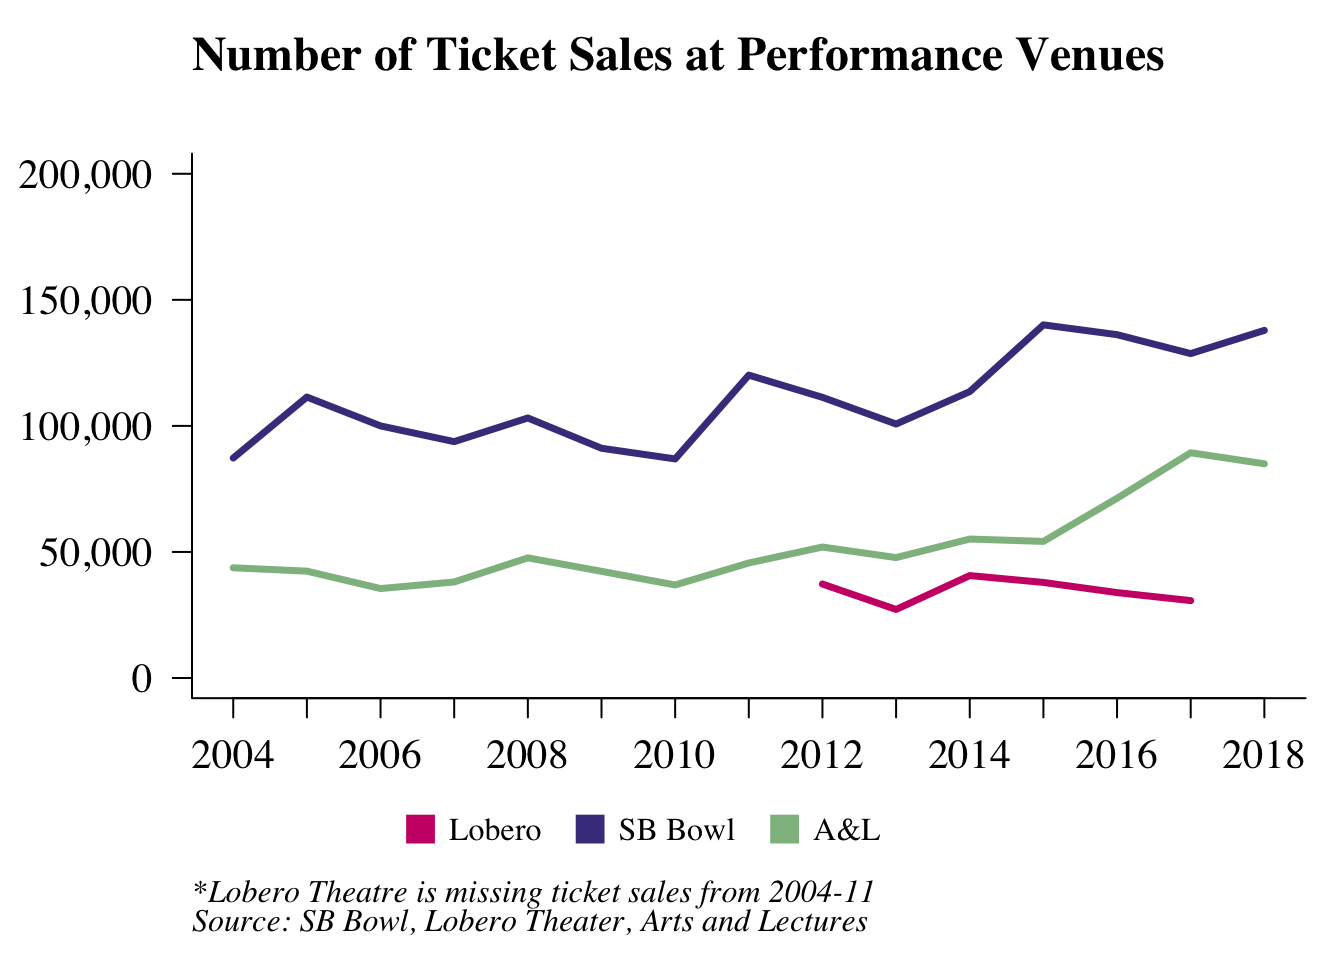
\includegraphics[width=0.95\linewidth]{cip_2019_files/figure-latex/unnamed-chunk-25-1}

\subsubsection*{What is the measure?}\label{what-is-the-measure-15}
\addcontentsline{toc}{subsubsection}{What is the measure?}

The percentage of high school seniors taking the SAT.

\subsubsection*{Why is it important?}\label{why-is-it-important-13}
\addcontentsline{toc}{subsubsection}{Why is it important?}

Taking the SAT exam is an indication that a student hopes to attend a
four-year college or university. Consequently, the percentage of
students taking the SAT is a measure of how successfully the schools
have prepared their students and of student aspirations. Paradoxically,
the higher the percentage of students taking the exam, the lower the
average SAT score tends to be because relatively weak students are
taking the exam.

\subsubsection*{How are we doing?}\label{how-are-we-doing-17}
\addcontentsline{toc}{subsubsection}{How are we doing?}

Despite a small drop in percentages for South Coast in the last year,
the trend of high school seniors taking the SAT appears to be rising
across all three locations. However, it is important to note that less
than half of high school students take the SAT, denoting those with
aspirations for a college or university degree directly after high
school.

\subsection*{SOUTH COAST OUTSCORES NORTH COUNTY ON
CAASPP}\label{south-coast-outscores-north-county-on-caaspp}
\addcontentsline{toc}{subsection}{SOUTH COAST OUTSCORES NORTH COUNTY ON
CAASPP}

\subsubsection*{What are the measures?}\label{what-are-the-measures-2}
\addcontentsline{toc}{subsubsection}{What are the measures?}

The California Assessment of Student Performance Progress (CAASPP) is a
newer program implemented to replace the Standardized Testing and
Reporting (STAR) exam system. Designed to measure understanding of
mathematical and verbal skills, the test is given to public school
students in the County and then compared to other students in
California.

\subsubsection*{Why is it important?}\label{why-is-it-important-14}
\addcontentsline{toc}{subsubsection}{Why is it important?}

Similar to the SAT, these tests are designed to measure the preparedness
and general education level of local students. The scores are also used
as a benchmark in assessing and comparing the performance of schools.

\subsubsection*{How are we doing?}\label{how-are-we-doing-18}
\addcontentsline{toc}{subsubsection}{How are we doing?}

All six elementary school districts in the South Coast outperform the
County in the percent of students that have met or exceeded the CAASPP
standard for both English and Math. However, the statewide test results
surpass those of the Santa Barbara and Carpinteria school districts. In
North County, only the Ballard, Buellton, Los Olivos, and Solvang school
districts score better than the California average.

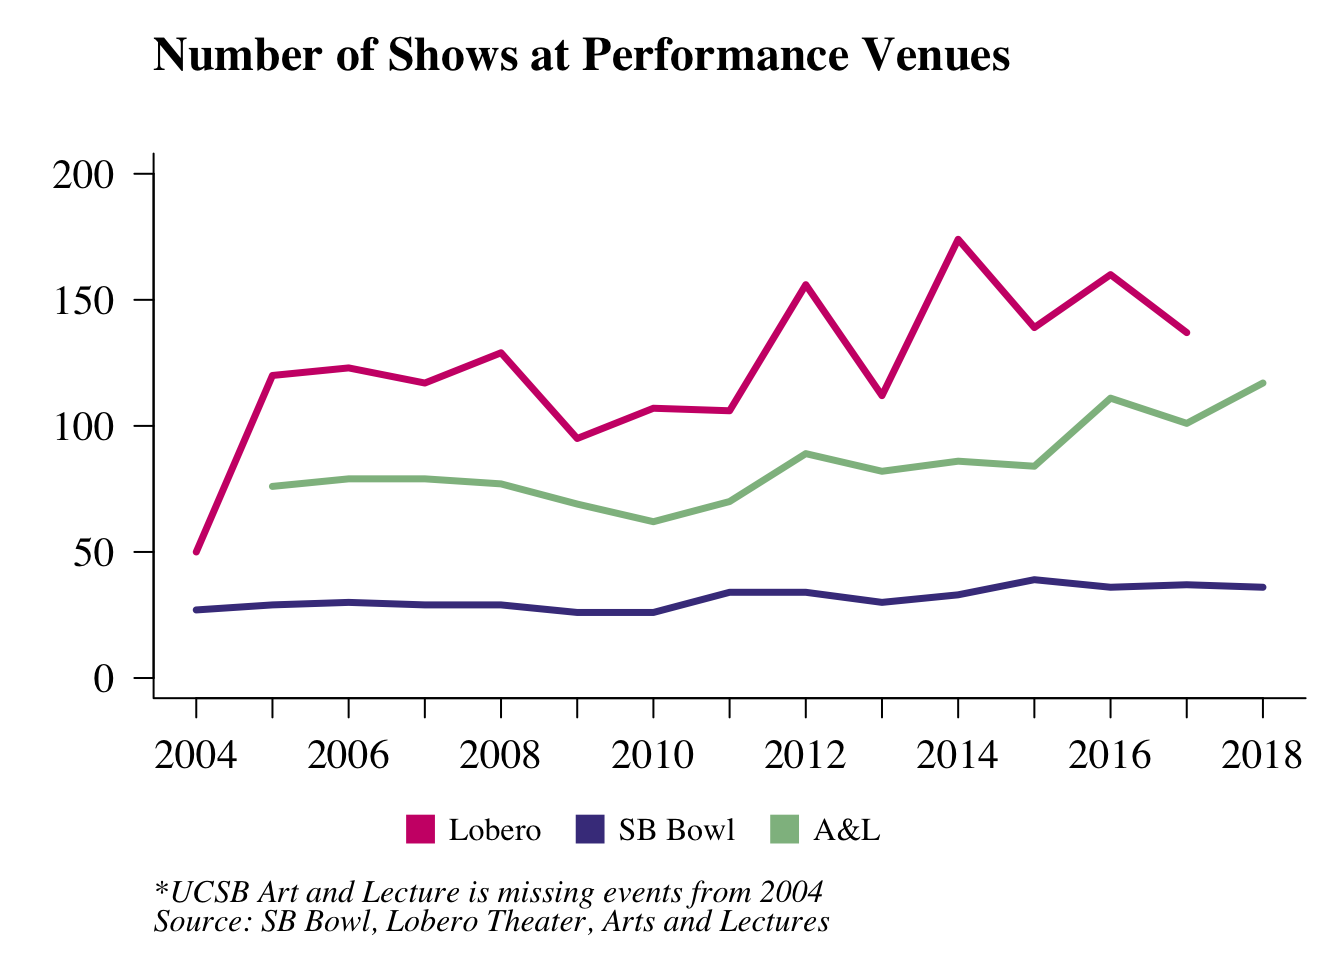
\includegraphics[width=0.95\linewidth]{cip_2019_files/figure-latex/unnamed-chunk-26-1}

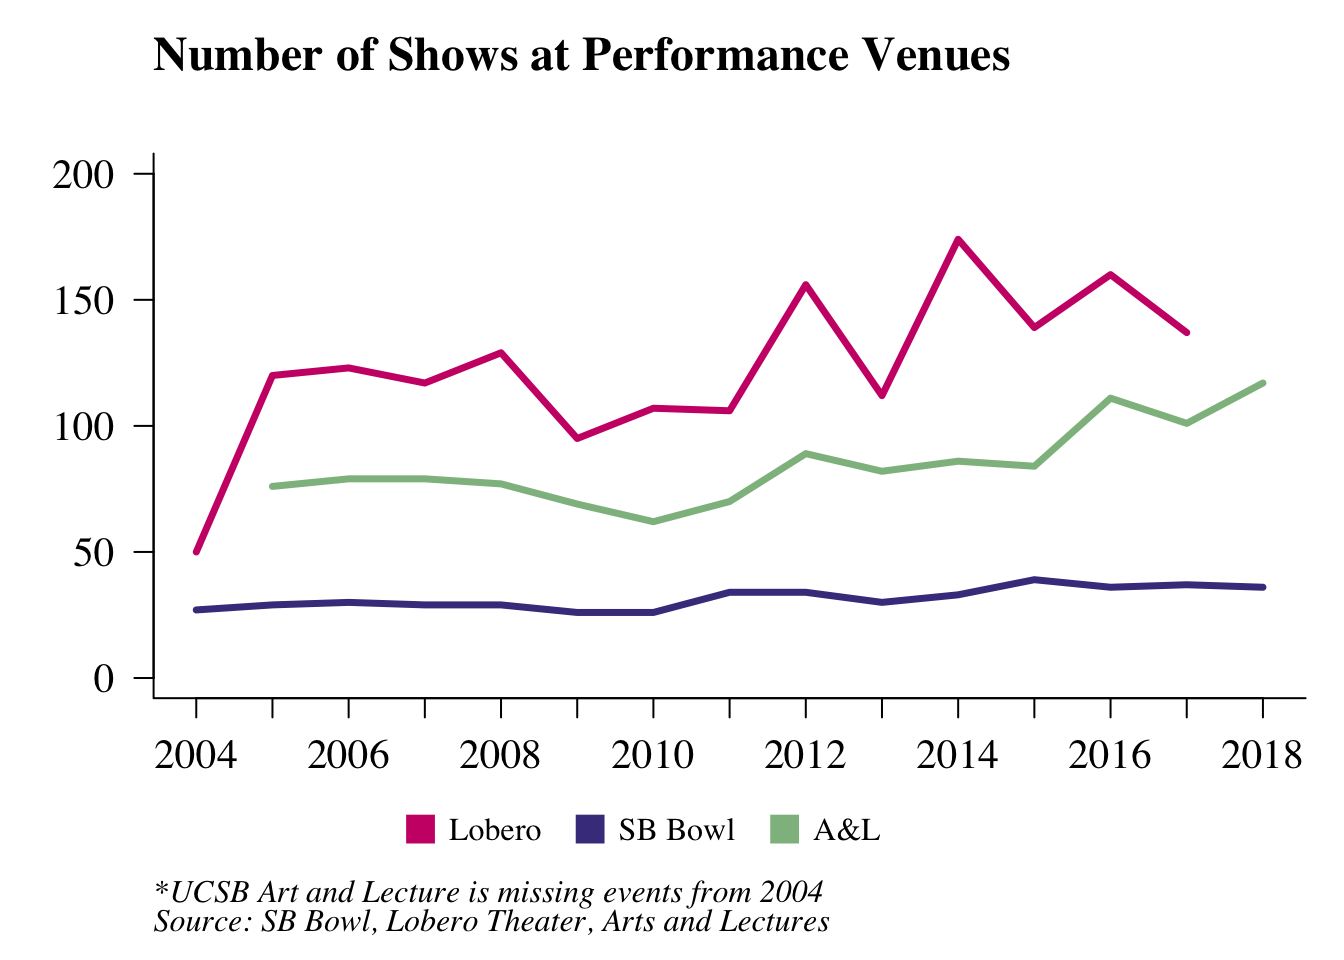
\includegraphics[width=0.95\linewidth]{cip_2019_files/figure-latex/unnamed-chunk-27-1}

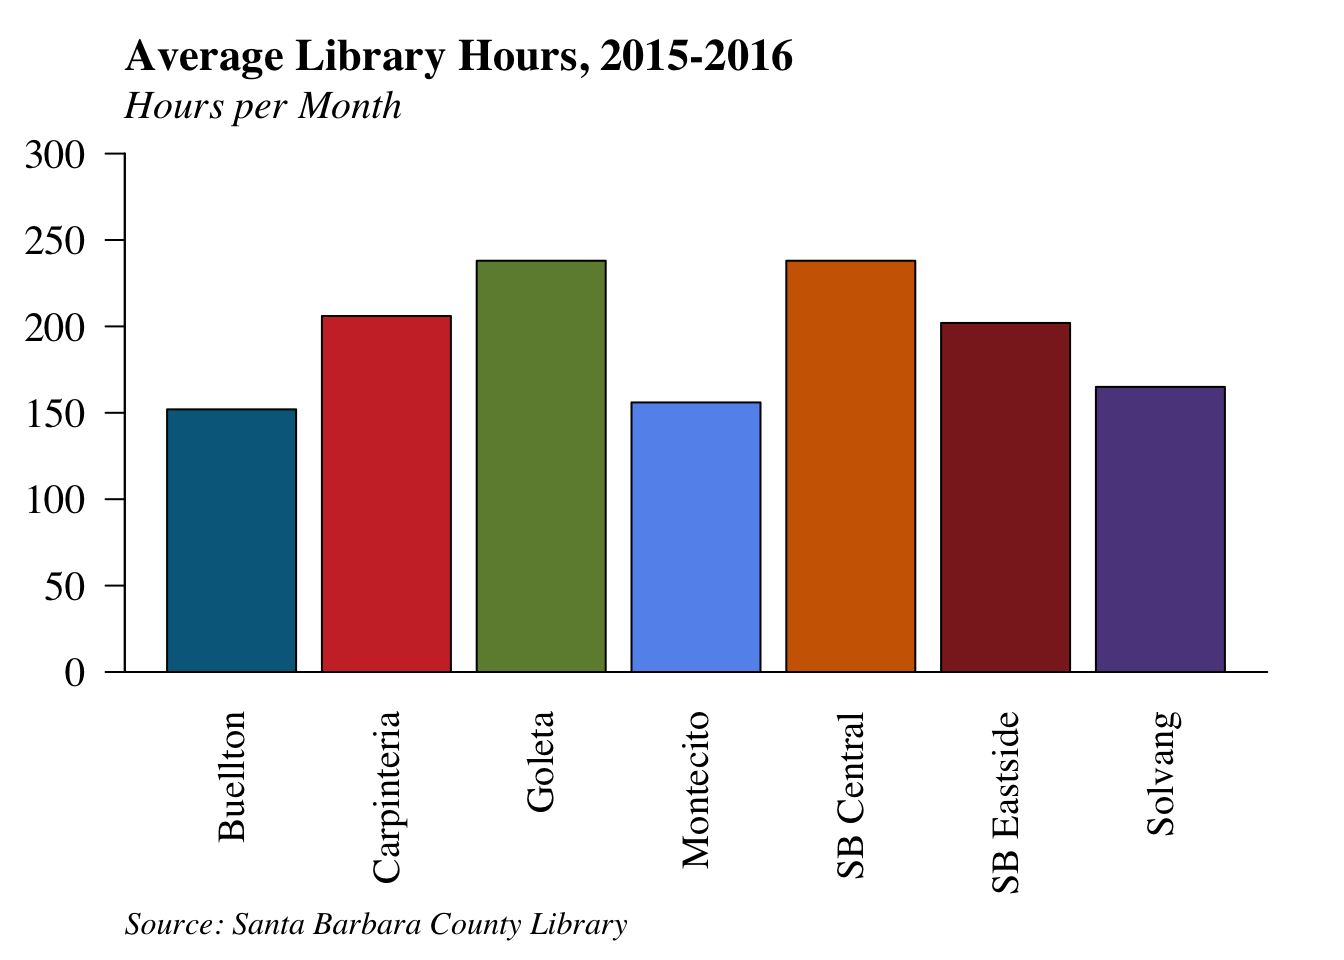
\includegraphics[width=0.95\linewidth]{cip_2019_files/figure-latex/unnamed-chunk-28-1}

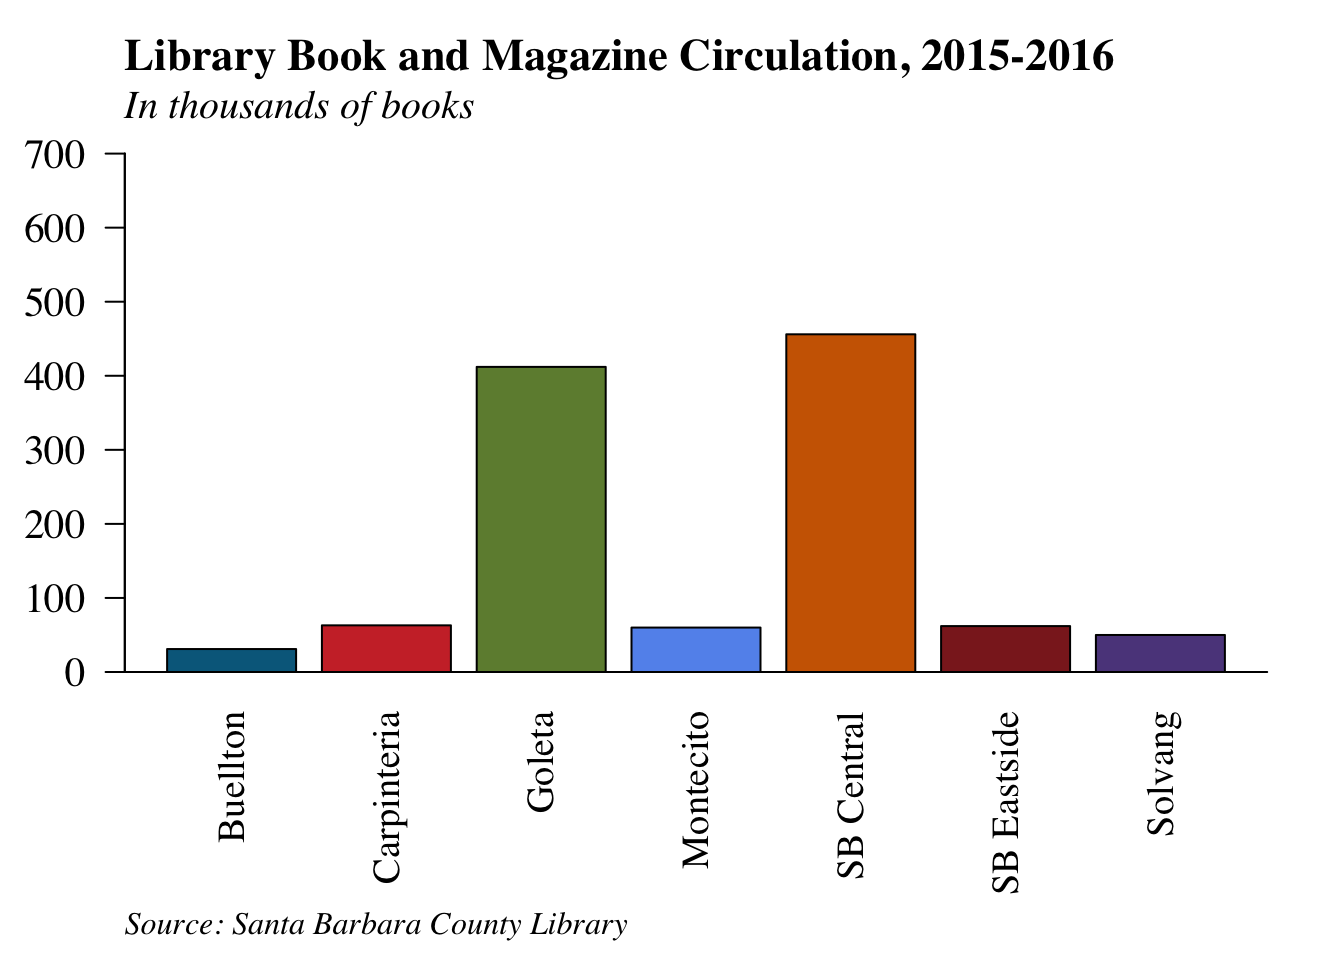
\includegraphics[width=0.95\linewidth]{cip_2019_files/figure-latex/unnamed-chunk-29-1}

\subsection*{BOOK AND MAGAZINE CIRCULATION SURPASSES ONE
MILLION}\label{book-and-magazine-circulation-surpasses-one-million}
\addcontentsline{toc}{subsection}{BOOK AND MAGAZINE CIRCULATION
SURPASSES ONE MILLION}

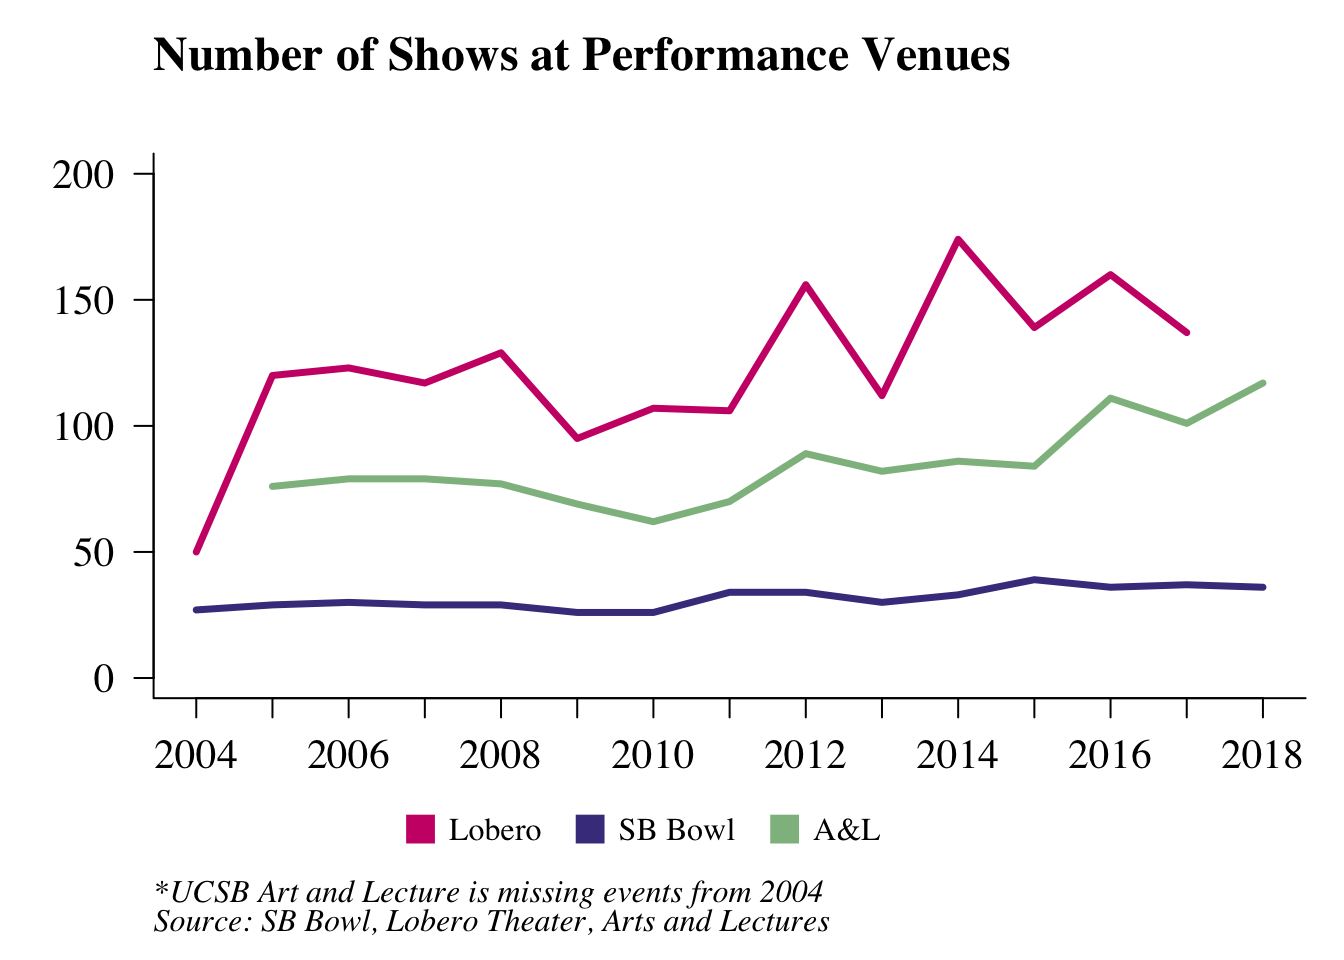
\includegraphics[width=0.95\linewidth]{cip_2019_files/figure-latex/unnamed-chunk-30-1}

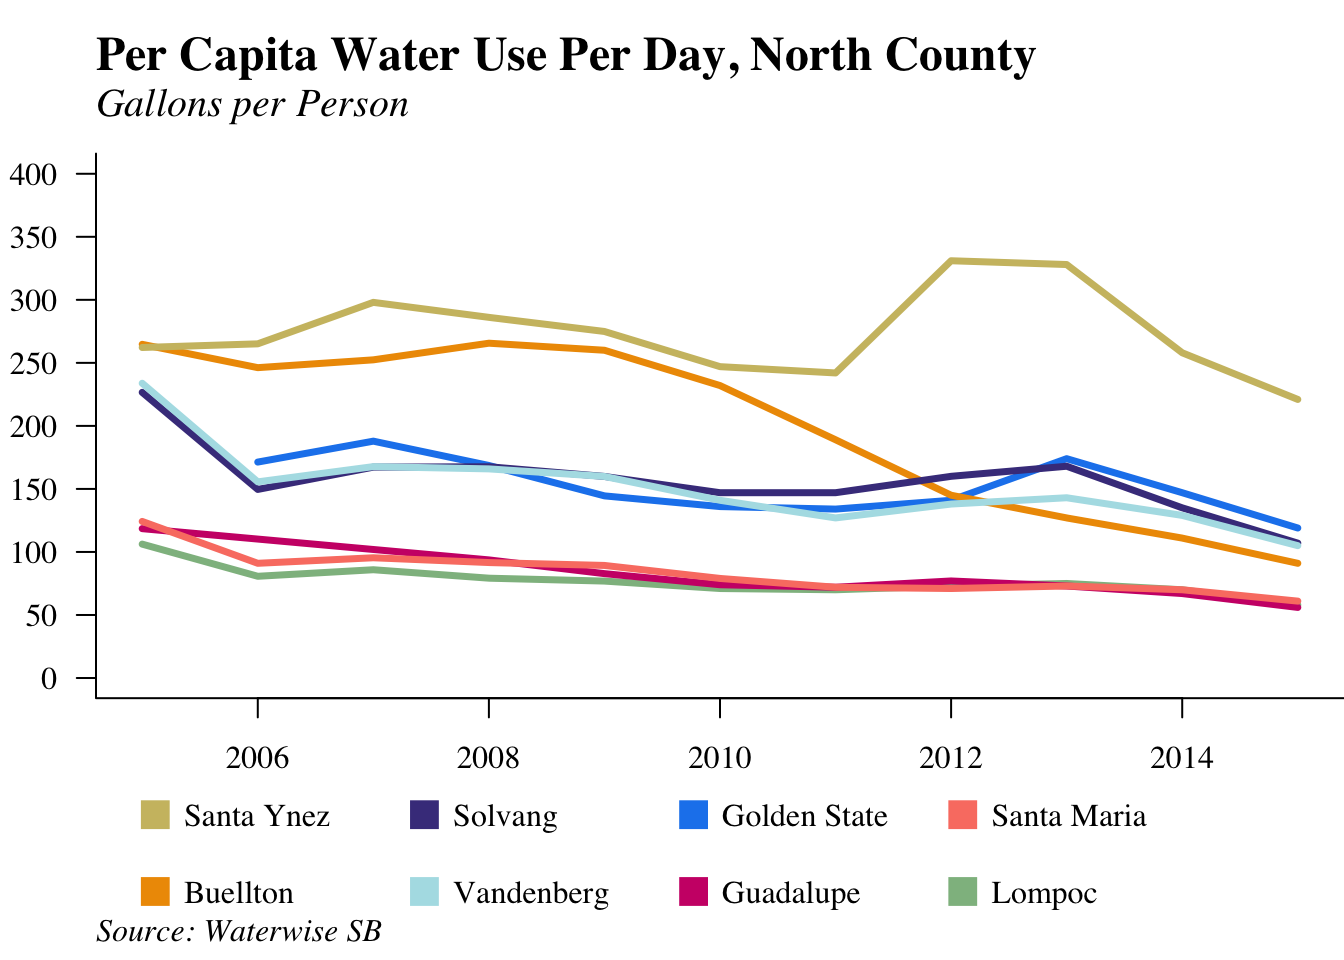
\includegraphics[width=0.95\linewidth]{cip_2019_files/figure-latex/unnamed-chunk-31-1}

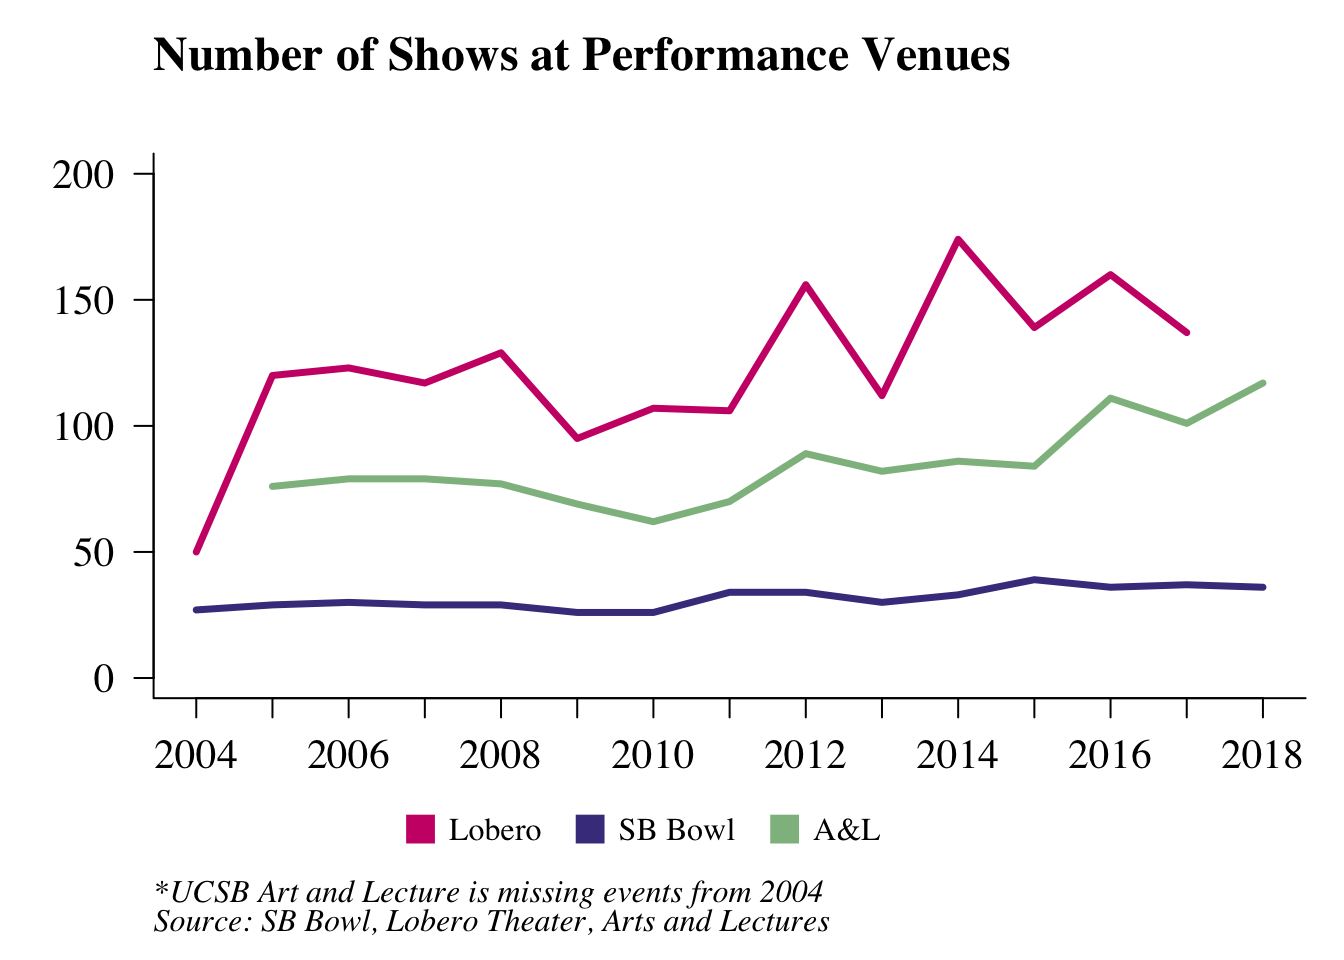
\includegraphics[width=0.95\linewidth]{cip_2019_files/figure-latex/unnamed-chunk-32-1}

\subsubsection*{What are the measures?}\label{what-are-the-measures-3}
\addcontentsline{toc}{subsubsection}{What are the measures?}

We are tracking three measures by sub-area in Santa Barbara County: the
volume of book and magazine circulation, the monthly average of library
hours, and the volume of library audio-visual circulation.

\subsubsection*{Why are they important?}\label{why-are-they-important-2}
\addcontentsline{toc}{subsubsection}{Why are they important?}

Public libraries provide supplemental educational resources for
children, continuing education opportunities for adults, and an
enhancement of the cultural quality of life.

\subsubsection*{How are we doing?}\label{how-are-we-doing-19}
\addcontentsline{toc}{subsubsection}{How are we doing?}

This data shows active use of library service throughout the Santa
Barbara County. The average library hours has remained unchanged over
the past three years. Meanwhile, book and magazine circulation surpassed
one million books, and audio-visual circulation was nearly half a
million units.

\section*{Citizen Engagement}\label{citizen-engagement}
\addcontentsline{toc}{section}{Citizen Engagement}

\subsection*{VOTER REGISTRATION AND TURNOUT
INCREASES}\label{voter-registration-and-turnout-increases}
\addcontentsline{toc}{subsection}{VOTER REGISTRATION AND TURNOUT
INCREASES}

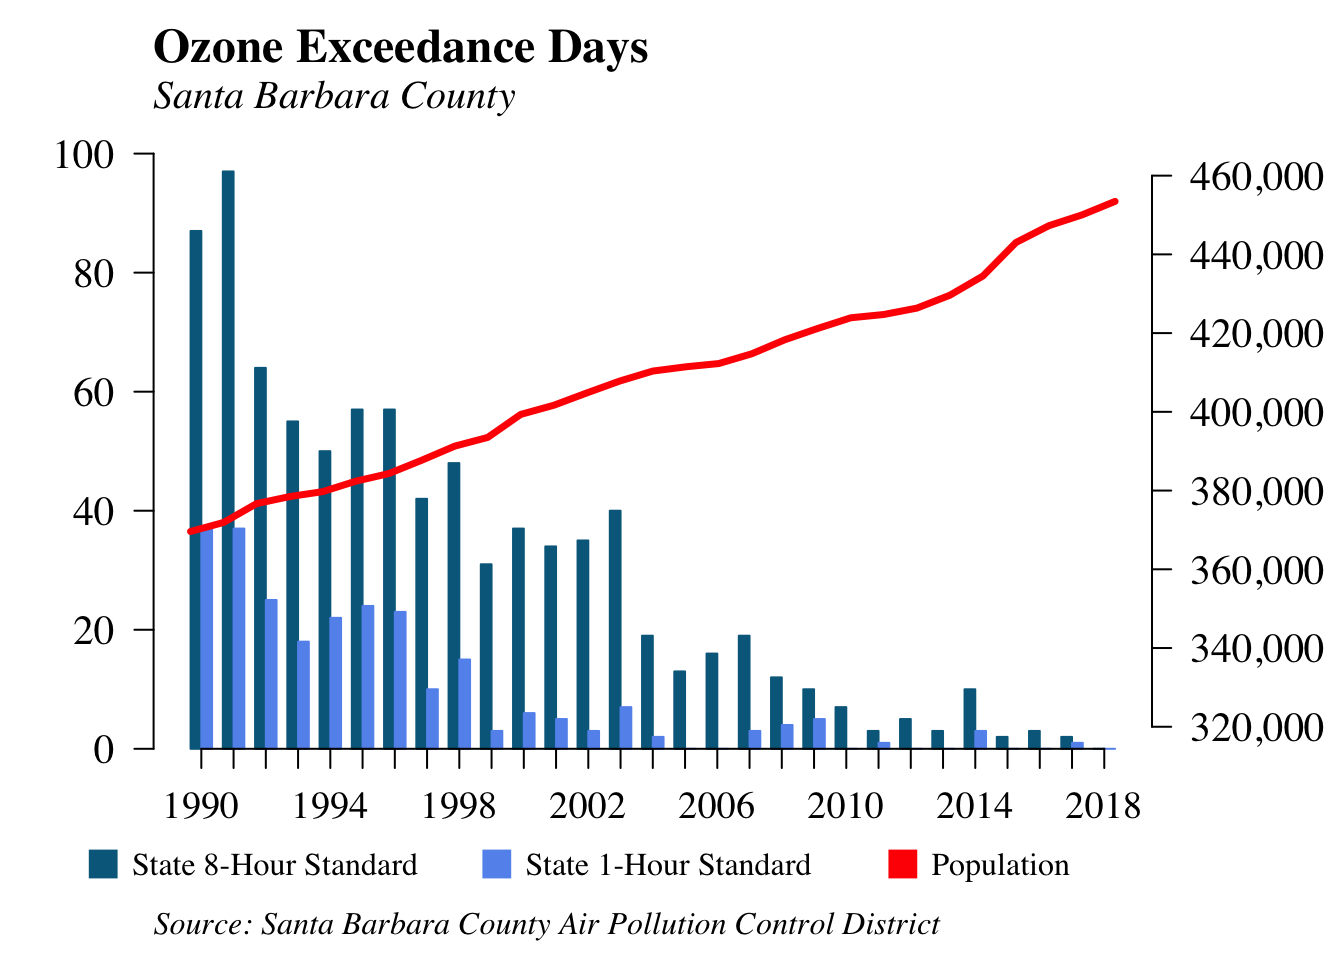
\includegraphics[width=1\linewidth]{cip_2019_files/figure-latex/unnamed-chunk-33-1}

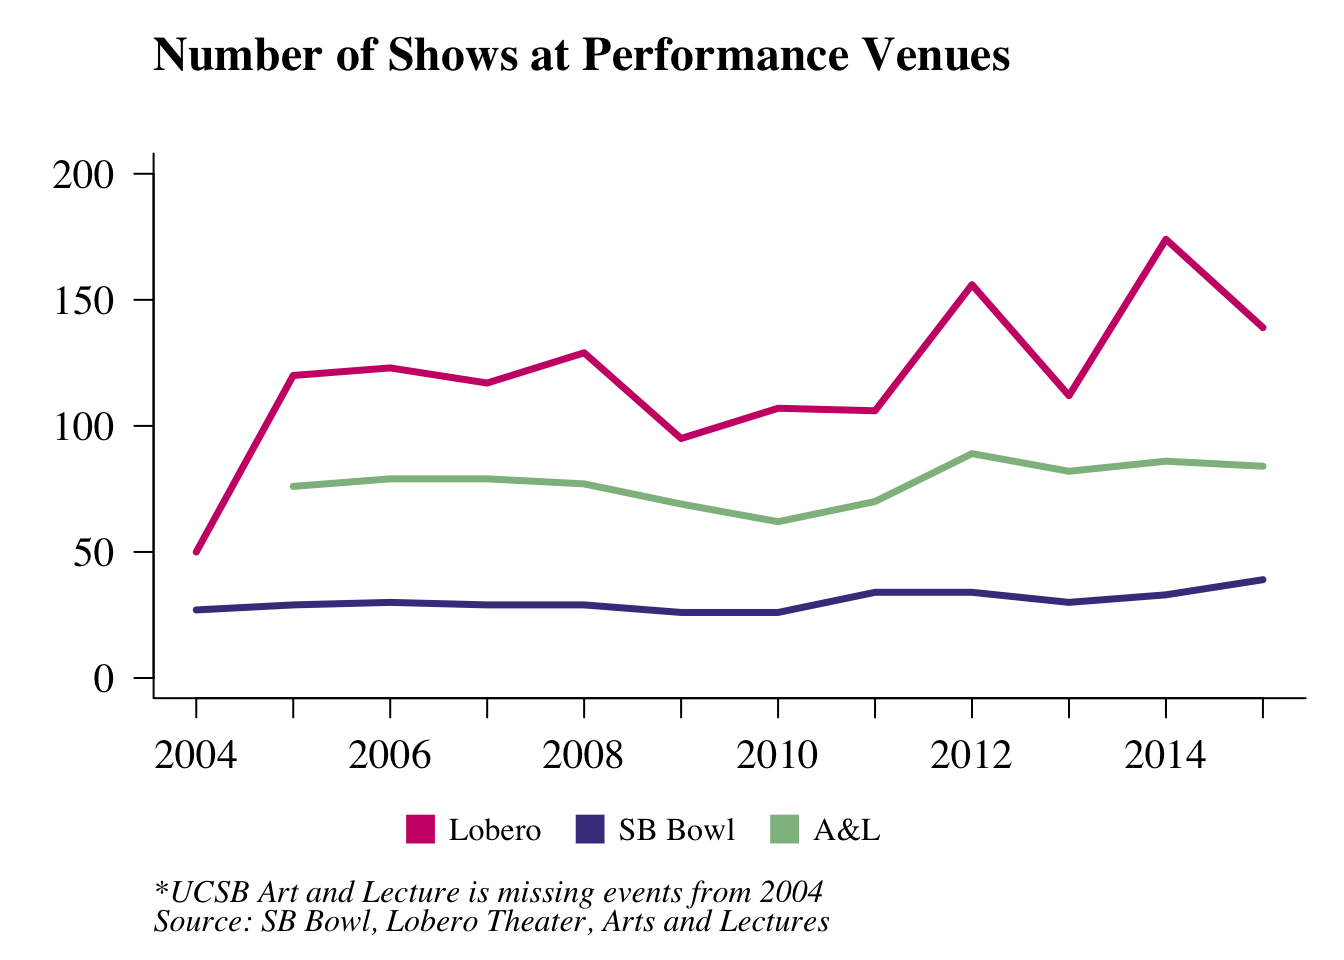
\includegraphics[width=1\linewidth]{cip_2019_files/figure-latex/unnamed-chunk-34-1}

\subsubsection*{What are the measures?}\label{what-are-the-measures-4}
\addcontentsline{toc}{subsubsection}{What are the measures?}

These graphs measure the percent of the eligible population that is
registered to vote and the percent of registered voters who voted in
past elections in Santa Barbara County.

\subsubsection*{Why are they important?}\label{why-are-they-important-3}
\addcontentsline{toc}{subsubsection}{Why are they important?}

Voter registration and turnout measure the most basic forms of civic
participation, and are surrogate measures for the level of interest
residents have in community affairs. Broad-based citizen involvement not
only improves the accountability of government, but also creates a
critical fabric of support for all our institutions.

\subsubsection*{How are we doing?}\label{how-are-we-doing-20}
\addcontentsline{toc}{subsubsection}{How are we doing?}

Voter registration increased in the 2016 Presidential Election, reaching
76.8 percent of eligible voters. This is the highest voter registration
percentage in recent election cycles since 2004, where voter
registration was 79.5 percent. The voter turnout for the presidential
election also increased from 80.3 percent in 2012 to 81.7 percent in
2016. However, voter turnout in midterm elections has been decreasing,
reaching its lowest levels of recent years in 2014.

\section*{Cultural Resources}\label{cultural-resources}
\addcontentsline{toc}{section}{Cultural Resources}

\subsection*{PERFORMING ARTS TICKET SALES INCREASE AS NUMBER OF SHOWS
SHOW A SLIGHT
DECLINE}\label{performing-arts-ticket-sales-increase-as-number-of-shows-show-a-slight-decline}
\addcontentsline{toc}{subsection}{PERFORMING ARTS TICKET SALES INCREASE
AS NUMBER OF SHOWS SHOW A SLIGHT DECLINE}

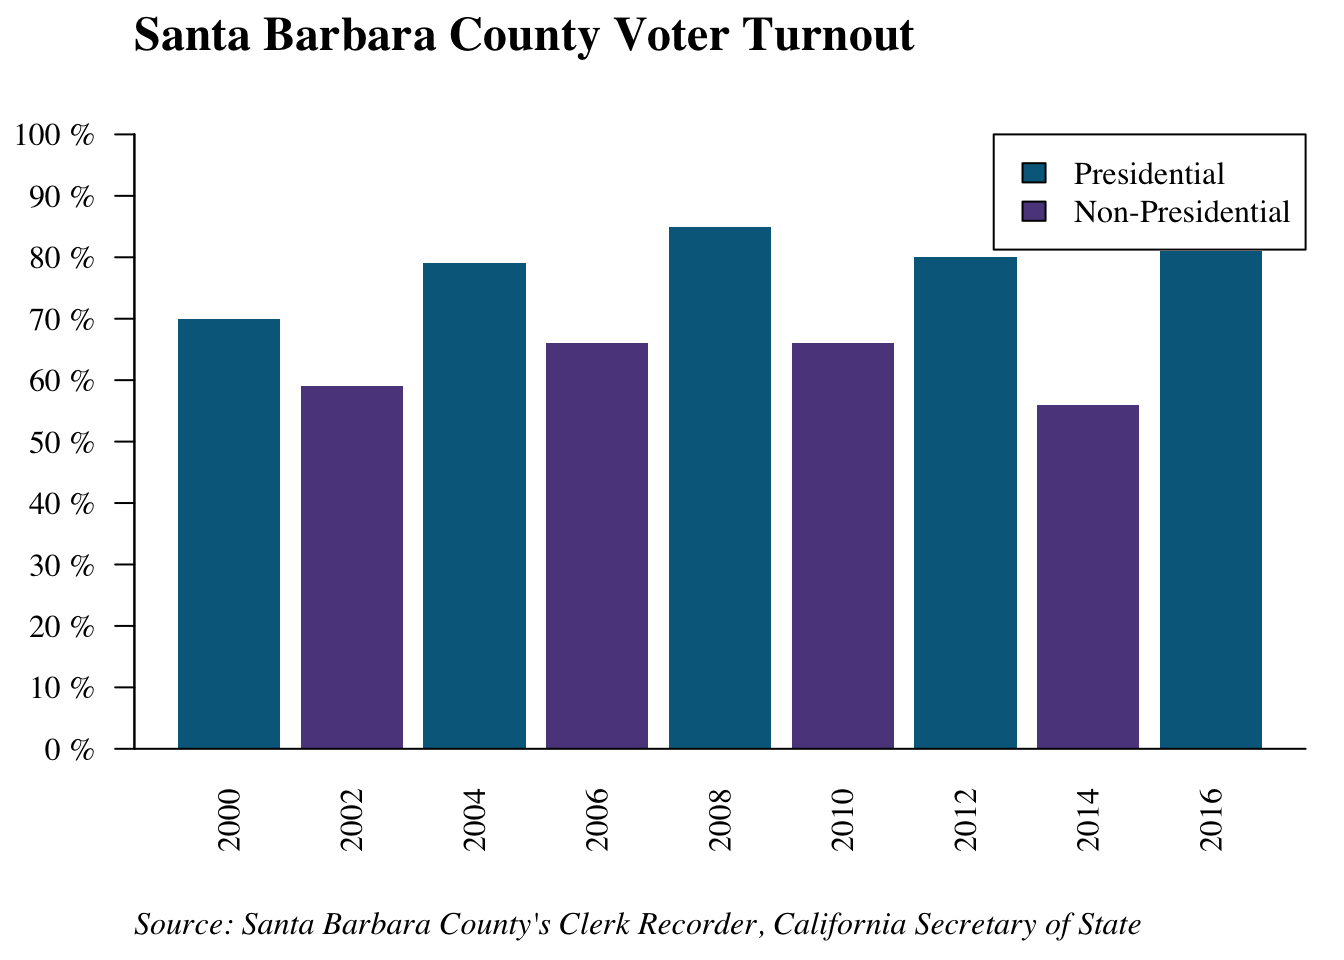
\includegraphics[width=1\linewidth]{cip_2019_files/figure-latex/unnamed-chunk-35-1}

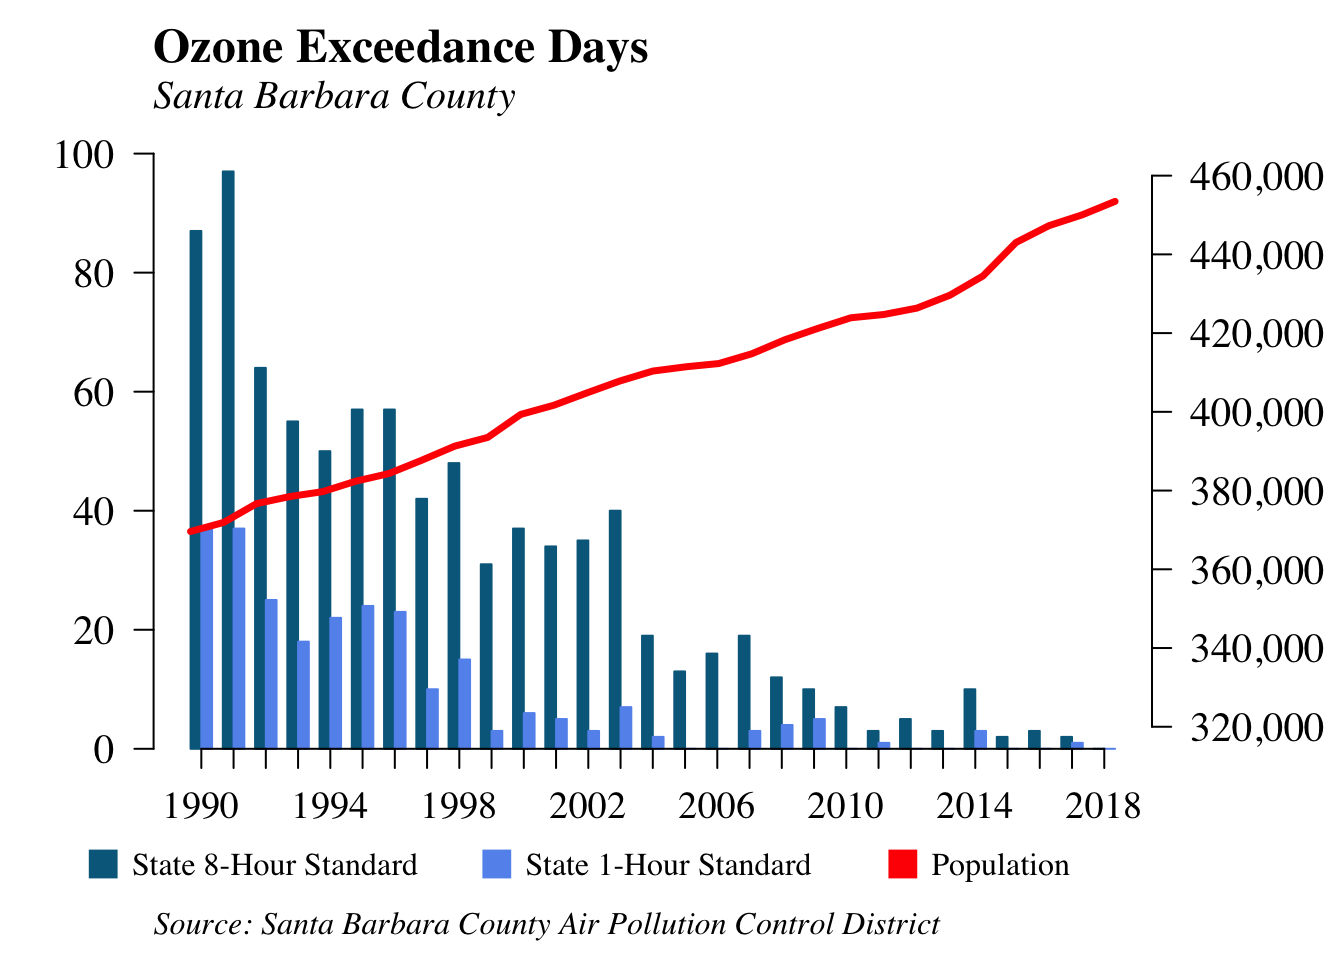
\includegraphics[width=1\linewidth]{cip_2019_files/figure-latex/unnamed-chunk-36-1}

\subsubsection*{What is the measure?}\label{what-is-the-measure-16}
\addcontentsline{toc}{subsubsection}{What is the measure?}

The total ticket sales and number of performances at the Santa Barbara
Bowl, the Lobero Theater, and UCSB Arts and Lectures.

\subsubsection*{Why is it important?}\label{why-is-it-important-15}
\addcontentsline{toc}{subsubsection}{Why is it important?}

The arts are a critical part of the community fabric that offers a place
where residents and visitors alike can come together, and enjoy the
artistic expression of the human spirit.

\subsubsection*{How are we doing?}\label{how-are-we-doing-21}
\addcontentsline{toc}{subsubsection}{How are we doing?}

Total tickets sales for all three venues in 2015 was 232,168 dispalying
an 11 percent increase from 2014; at the same time, the total number of
shows declined 10\%. Santa Barbara Bowl experienced a 23 percent spike
in ticket sales, along with an increase of 6 events. Lobero Theater saw
a decline of 7\% in ticket sales corresponding with a 20 percent
decrease of events throughout 2015. Similiarly, UCSB Arts and Lectures
displayed a loss in ticket sales, but with roughly the same amount of
events from the previous year.

\chapter*{Environmental}\label{environmental}
\addcontentsline{toc}{chapter}{Environmental}

\section*{Water Quality}\label{water-quality}
\addcontentsline{toc}{section}{Water Quality}

\subsection*{WATER QUALITY VIOLATION DAYS RELATIVELY
STABLE}\label{water-quality-violation-days-relatively-stable}
\addcontentsline{toc}{subsection}{WATER QUALITY VIOLATION DAYS
RELATIVELY STABLE}

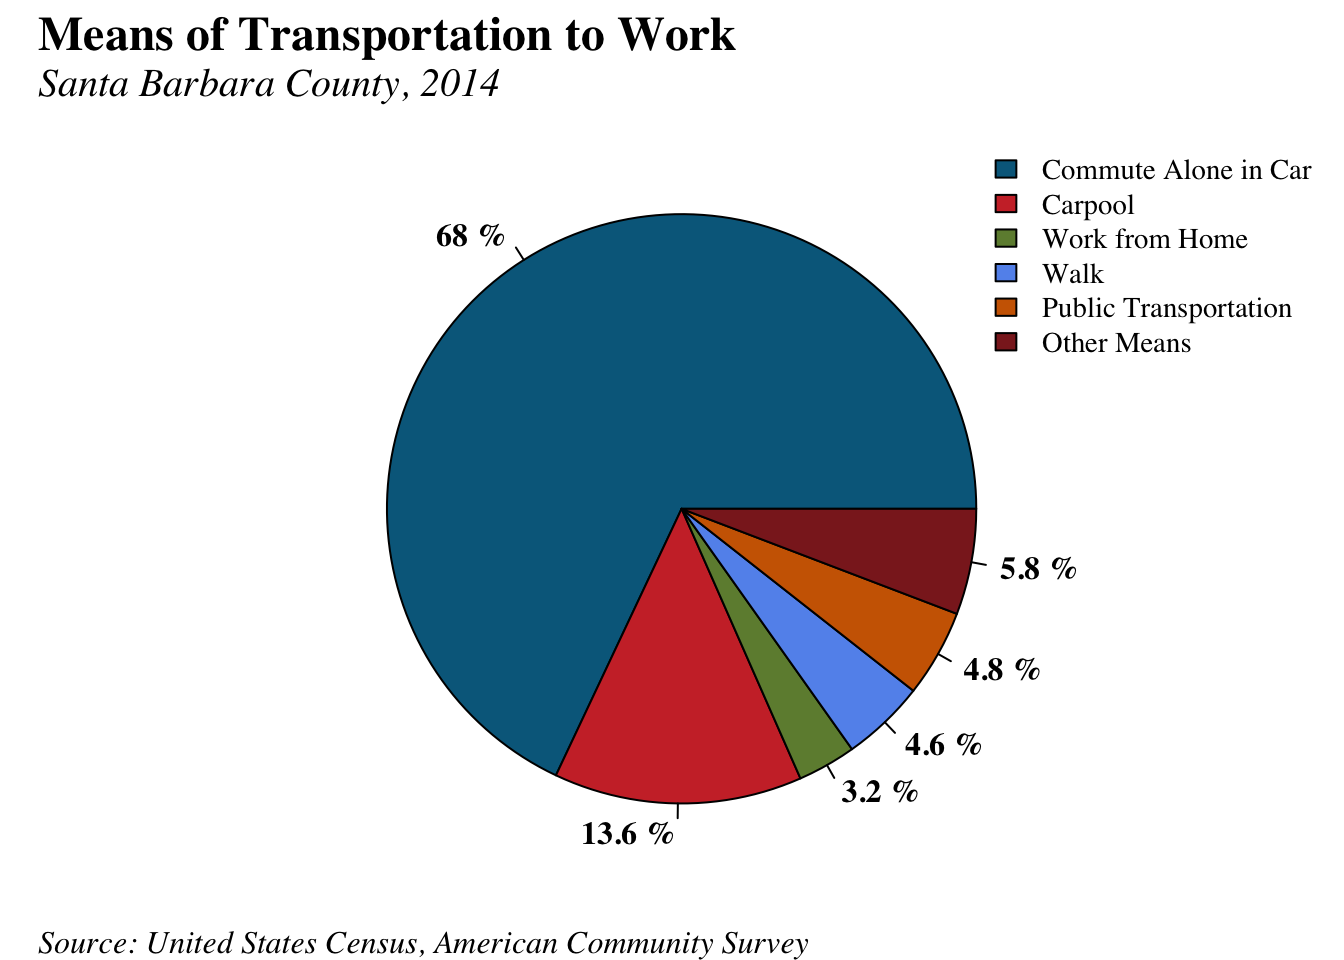
\includegraphics[width=0.95\linewidth]{cip_2019_files/figure-latex/unnamed-chunk-39-1}

\subsubsection*{What are the measures?}\label{what-are-the-measures-5}
\addcontentsline{toc}{subsubsection}{What are the measures?}

The percentage of weekly water quality tests that exceed state and
federal standards for fecal coliform and enterococcus. This data is from
the County Ocean Water Monitoring Program, which tests ocean water near
the mouth of most major creeks in the Santa Barbara County. A reading of
more than 400 parts per million for fecal coliform, 104 for
enterococcus, or 10,000 MPN (Most Probable Number, meaning the bacterial
count per 100 mL of water) for total coliform exceeds state and federal
standards, and can lead to a Department of Environmental Health Beach
Advisory.

\subsubsection*{Why are they important?}\label{why-are-they-important-4}
\addcontentsline{toc}{subsubsection}{Why are they important?}

The quality of water coming out of a watershed directly reflects what
goes into the watershed and is an indicator of the watershed's overall
health. This not only affects the ability of residents to enjoy local
creeks and beaches, but also affects the health of wildlife. In
addition, unsafe beaches can adversely impact the local economy by
reducing tourism.

\subsubsection*{How are we doing?}\label{how-are-we-doing-22}
\addcontentsline{toc}{subsubsection}{How are we doing?}

Water quality violation days have remained relatively stable over the
last five years, though there was a small increase in fecal coliform.
Still, less than ten percent of tests had results where bacteria
exceeded state and federal standards. The amount of rainfall can
significantly affect these results, as rainfall flushes bacteria and
pollutants from the creeks into the ocean.

\subsection*{WATER CONSUMPTION
DECLINES}\label{water-consumption-declines}
\addcontentsline{toc}{subsection}{WATER CONSUMPTION DECLINES}

\subsubsection*{What is the measure?}\label{what-is-the-measure-17}
\addcontentsline{toc}{subsubsection}{What is the measure?}

The amount of gallons of water consumed per day for residential purposes
by the customers of all the principal water agencies within the Santa
Barbara County.

\subsubsection*{Why is it important?}\label{why-is-it-important-16}
\addcontentsline{toc}{subsubsection}{Why is it important?}

The amount of water consumed by residents of Santa Barbara County is
especially important in times of drought conditions. The County has
taken several steps to reduce residential water consumption, which
appears to have had a positive effect on lowering water usage.

\subsubsection*{How are we doing?}\label{how-are-we-doing-23}
\addcontentsline{toc}{subsubsection}{How are we doing?}

The current drought has reduced countywide water consumption, with
marked decreases beginning in 2013. Montecito, Santa Ynez, and La Cumbre
continue to have the highest personal consumption of water out of the
County, whereas Guadalupe, Santa Maria, Lompoc, Goleta, Carpinteria, and
Santa Barbara have the lowest per capita water consumption in the
county. Residential water consumption is at its lowest rate in ten
years.

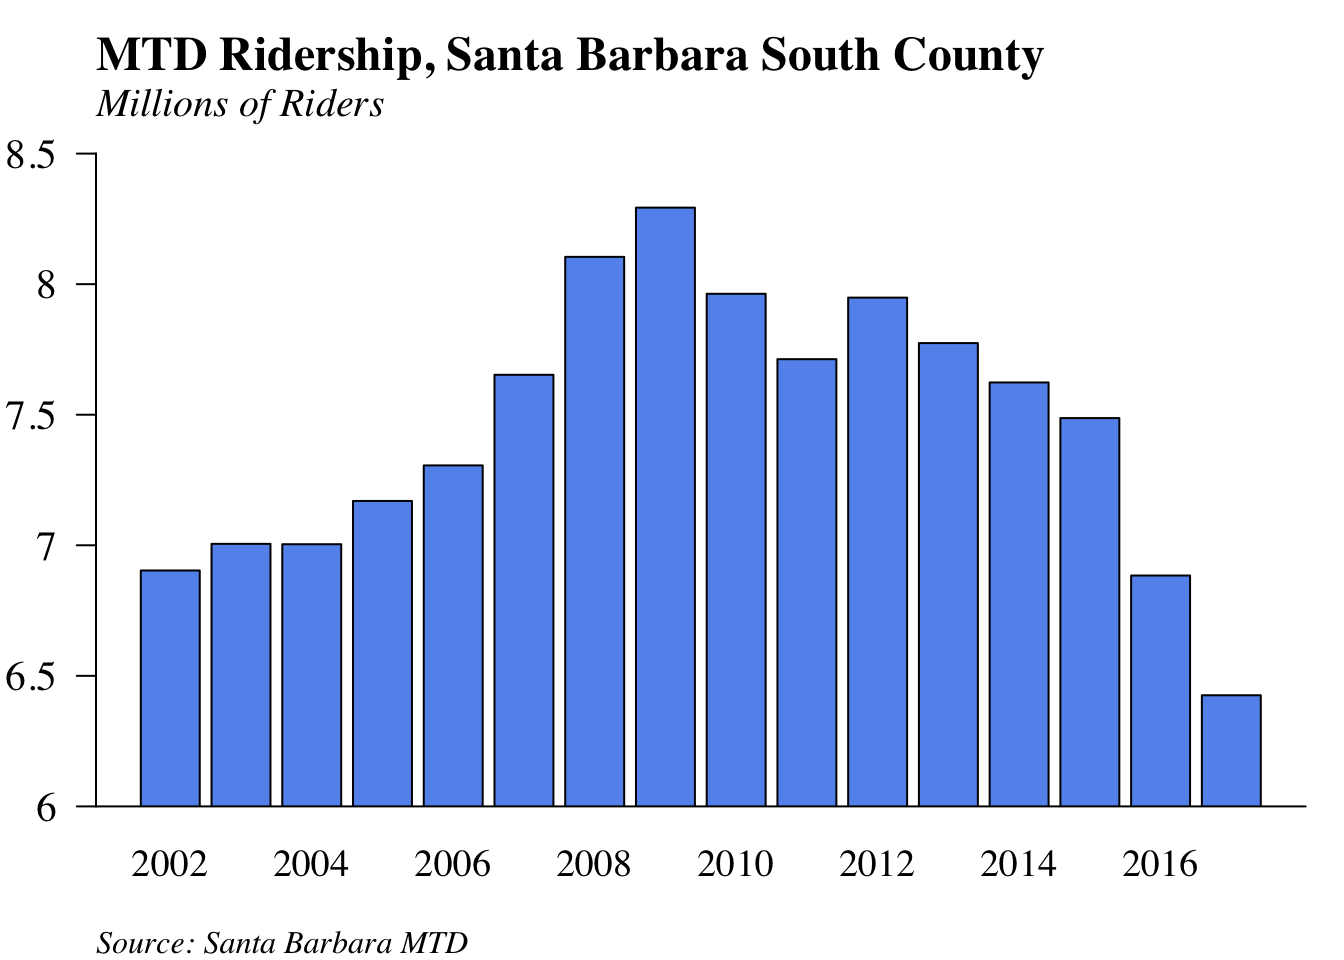
\includegraphics[width=0.95\linewidth]{cip_2019_files/figure-latex/unnamed-chunk-41-1}

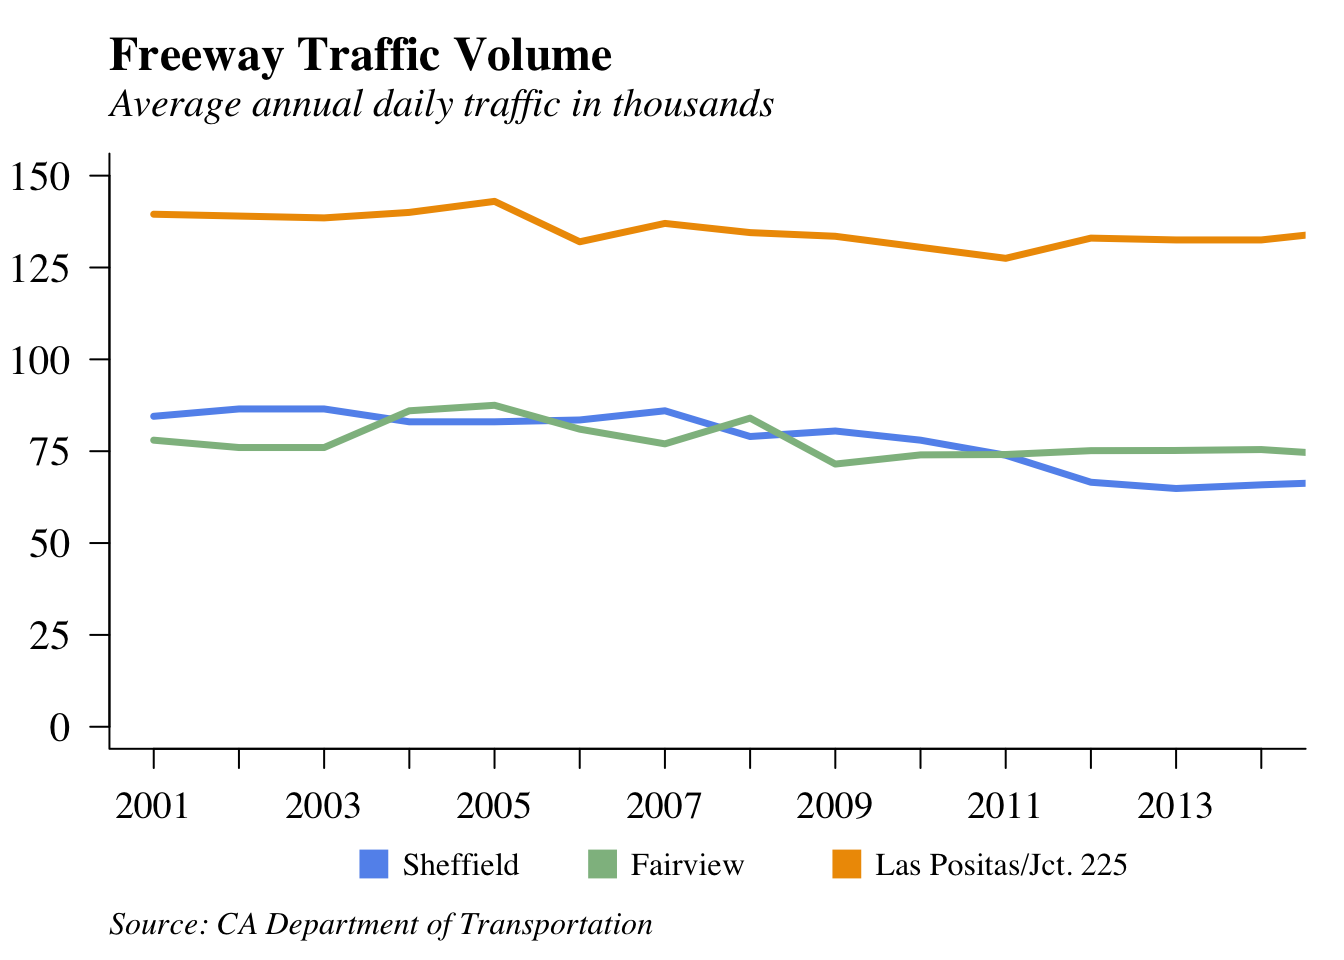
\includegraphics[width=0.95\linewidth]{cip_2019_files/figure-latex/unnamed-chunk-42-1}

\section*{Air Quality}\label{air-quality}
\addcontentsline{toc}{section}{Air Quality}

\subsection*{OZONE VIOLATION DAYS SIGNIFICANTLY
REDUCED}\label{ozone-violation-days-significantly-reduced}
\addcontentsline{toc}{subsection}{OZONE VIOLATION DAYS SIGNIFICANTLY
REDUCED}

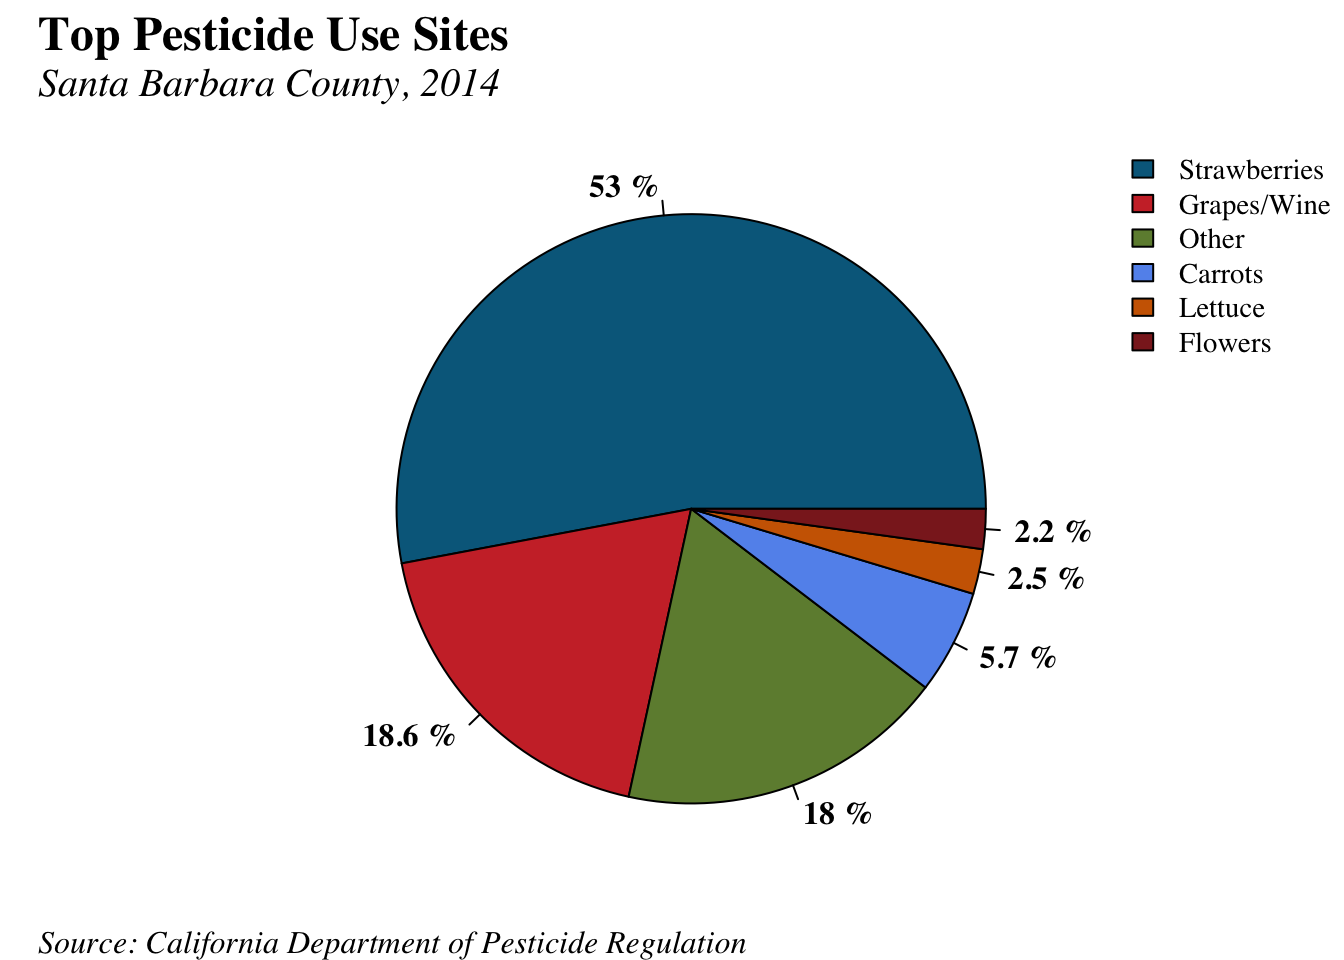
\includegraphics[width=0.95\linewidth]{cip_2019_files/figure-latex/unnamed-chunk-43-1}

\subsubsection*{What is the measure?}\label{what-is-the-measure-18}
\addcontentsline{toc}{subsubsection}{What is the measure?}

The number of days in which local communities did not meet the state
standard for ozone levels. If a daily ozone reading exceeds an hourly
average of 0.09 parts per million, or an eight hour average of 0.07
parts per million, a state ``violation day'' occurs.

\subsubsection*{Why is it important?}\label{why-is-it-important-17}
\addcontentsline{toc}{subsubsection}{Why is it important?}

Ozone -- one of the primary components of smog -- impairs normal
functioning of the lungs and reduces the ability to perform physical
exercise. Lack of ozone in the air is considered to be a good indicator
of overall air quality.

\subsubsection*{How are we doing?}\label{how-are-we-doing-24}
\addcontentsline{toc}{subsubsection}{How are we doing?}

In 2016, Santa Barbara County only experienced three days of ozone
violation where the air quality exceeded the state 8-hour standard.
While this is an increase of one day from 2015 statistics, air quality
has improved dramatically over the past twenty years, even despite a
rise in population. In October 2015, the EPA passed a new federal
mandate reducing the 8-hour ozone violation from 0.075 parts per million
to 0.070 parts per million. Santa Barbara County is currently in
attainment of the 8-hour federal ozone standard.

\subsection*{NO BUSINESSES RELEASE TOXIC AIR POLLUTANTS IN
2015}\label{no-businesses-release-toxic-air-pollutants-in-2015}
\addcontentsline{toc}{subsection}{NO BUSINESSES RELEASE TOXIC AIR
POLLUTANTS IN 2015}

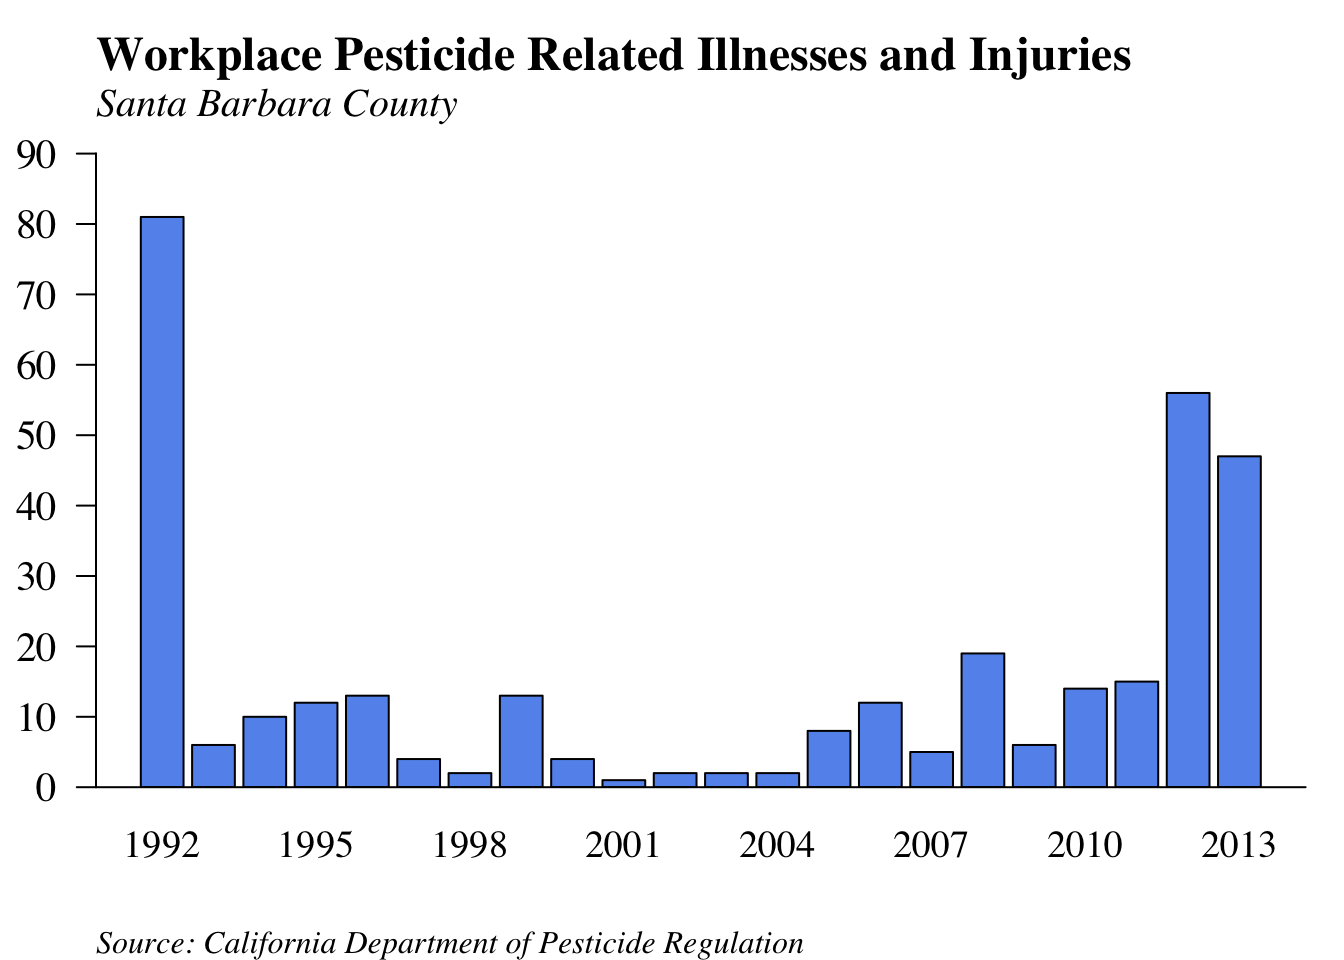
\includegraphics[width=0.95\linewidth]{cip_2019_files/figure-latex/unnamed-chunk-44-1}

\subsubsection*{What is the measure?}\label{what-is-the-measure-19}
\addcontentsline{toc}{subsubsection}{What is the measure?}

The number of businesses in Santa Barbara County that release airborne
toxic contaminants which exceed the Santa Barbara County Air Pollution
Control District's thresholds for significant health risks. Three
categories of toxic chemicals are measured -- those that pose cancer
risks, those that pose acute health risks, and those that pose chronic
health risks unrelated to cancer.

\subsubsection*{Why is it important?}\label{why-is-it-important-18}
\addcontentsline{toc}{subsubsection}{Why is it important?}

Toxic air contaminants pose a direct threat to the health of people who
work at businesses that exceed safety thresholds and to those who live
or work immediately adjacent to those businesses. In addition, the toxic
contaminants harm overall air quality in the Santa Barbara County.

\subsubsection*{How are we doing?}\label{how-are-we-doing-25}
\addcontentsline{toc}{subsubsection}{How are we doing?}

The number of businesses exceeding health risk thresholds has dropped to
zero in 2015. This is even more significant when stricter changes in
guidelines are taken into account; in 2003, the Office of Environmental
Health Hazard Assessment revised the guidance manual to account for
sensitivity to cancer at early ages, possibly resulting in increased
risk results.

\section*{Land Use}\label{land-use}
\addcontentsline{toc}{section}{Land Use}

\subsection*{PESTICIDE USE RISES SLIGHTLY OVER PAST
YEAR}\label{pesticide-use-rises-slightly-over-past-year}
\addcontentsline{toc}{subsection}{PESTICIDE USE RISES SLIGHTLY OVER PAST
YEAR}

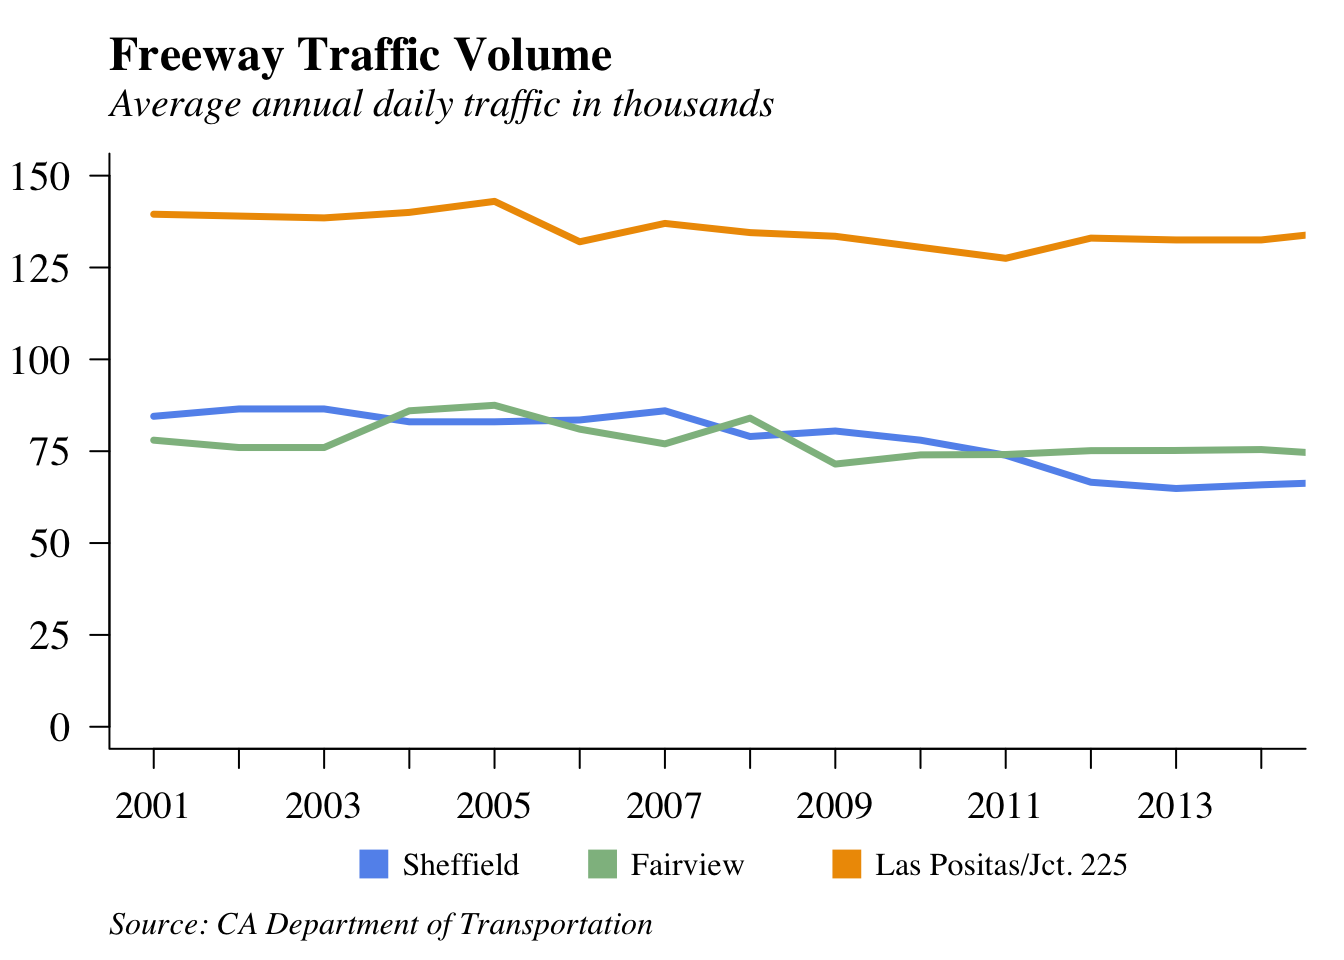
\includegraphics[width=0.95\linewidth]{cip_2019_files/figure-latex/unnamed-chunk-45-1}

\subsubsection*{What is the measure?}\label{what-is-the-measure-20}
\addcontentsline{toc}{subsubsection}{What is the measure?}

The total pounds of pesticide used in agriculture throughout Santa
Barbara County.

\subsubsection*{Why is it important?}\label{why-is-it-important-19}
\addcontentsline{toc}{subsubsection}{Why is it important?}

Many activities can affect ground and groundwater quality, most of which
are difficult to track. Agricultural pesticide use is one possible
precursor to ground or groundwater contamination. Pesticide use in the
county is mostly within North County.

\subsubsection*{How are we doing?}\label{how-are-we-doing-26}
\addcontentsline{toc}{subsubsection}{How are we doing?}

After a large spike in pesticide use in 2012 -- amounting to 6.18
million pounds -- its use declined significantly in 2013. Since then, it
has increased slightly to 4.78 million pounds. The lowest levels of
pesticide usage were observed in 2009, with only 3.73 million pounds.

\subsection*{STRAWBERRIES DOMINATE PESTICIDE USE
SITES}\label{strawberries-dominate-pesticide-use-sites}
\addcontentsline{toc}{subsection}{STRAWBERRIES DOMINATE PESTICIDE USE
SITES}

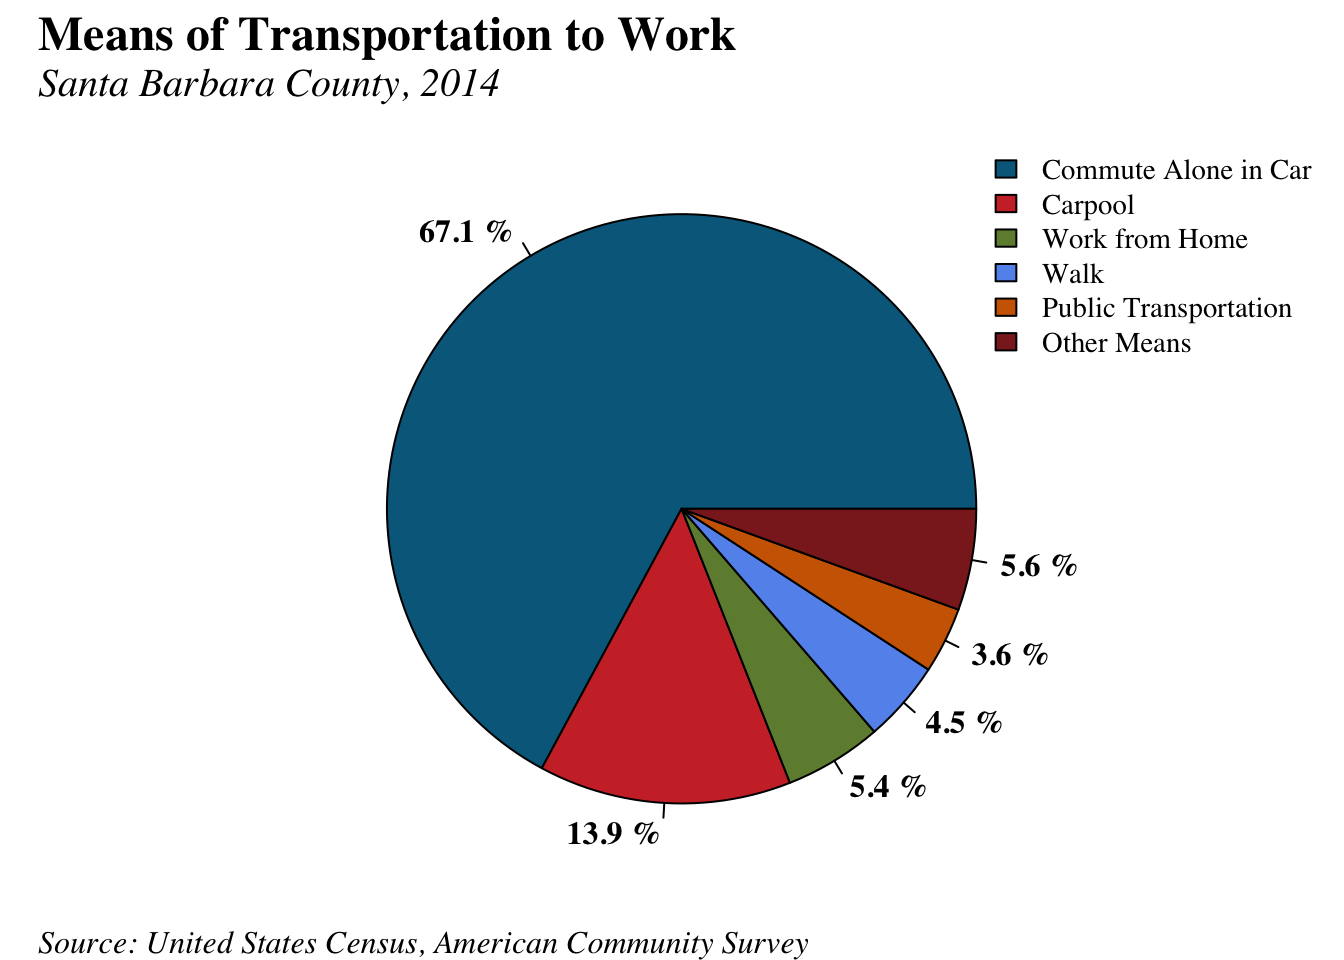
\includegraphics[width=0.95\linewidth]{cip_2019_files/figure-latex/unnamed-chunk-46-1}

\subsubsection*{What is the measure?}\label{what-is-the-measure-21}
\addcontentsline{toc}{subsubsection}{What is the measure?}

The top five sites of pesticide use throughout Santa Barbara County in
2014.

\subsubsection*{Why is it important?}\label{why-is-it-important-20}
\addcontentsline{toc}{subsubsection}{Why is it important?}

Countywide pesticide use totaled 4,782,176 pounds in 2014. Of that, five
types of crops constituted 82 percent of all pesticide use. These crops
may be located in specific agricultural areas where pesticide use
becomes more concentrated.

\subsubsection*{How are we doing?}\label{how-are-we-doing-27}
\addcontentsline{toc}{subsubsection}{How are we doing?}

The strawberry crop is the leading site for pesticide use in Santa
Barbara County, with 2,532,990 pounds of pesticides used in 2014. From
2013 to 2014, raspberries and lemons fell from the top pesticide sites
and were replaced by lettuce and flowers.

\subsection*{WORKPLACE PESTICIDE RELATED ILLNESSES AND INJURIES
INCREASE}\label{workplace-pesticide-related-illnesses-and-injuries-increase}
\addcontentsline{toc}{subsection}{WORKPLACE PESTICIDE RELATED ILLNESSES
AND INJURIES INCREASE}

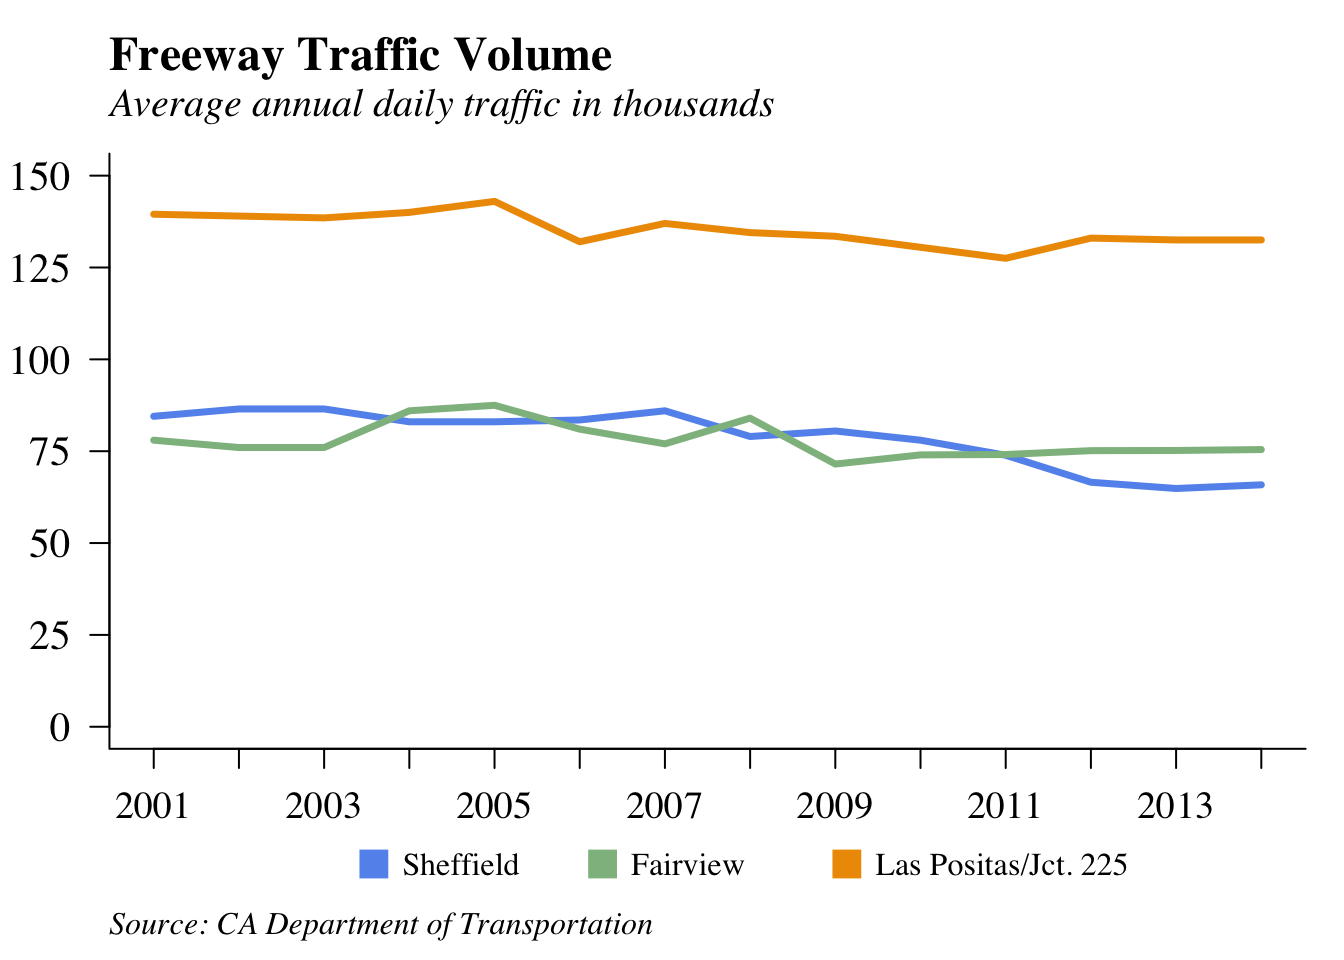
\includegraphics[width=0.95\linewidth]{cip_2019_files/figure-latex/unnamed-chunk-47-1}

\subsubsection*{What is the measure?}\label{what-is-the-measure-22}
\addcontentsline{toc}{subsubsection}{What is the measure?}

The number of workplace pesticide related illnesses and injuries
experienced in the Santa Barbara County. This measure includes
antimicrobial agents such as chlorine.

\subsubsection*{Why is it important?}\label{why-is-it-important-21}
\addcontentsline{toc}{subsubsection}{Why is it important?}

Many factors influence our health, including environmental factors.
Workplace pesticide related illnesses are one of those that are
regularly tracked.

\subsubsection*{How are we doing?}\label{how-are-we-doing-28}
\addcontentsline{toc}{subsubsection}{How are we doing?}

The number of reported illnesses related to pesticides has typically
remained under 20 cases a year, with three major exceptions. The past
two years saw a dramatic increase in the number of workplace pesticide
related illnesses. From 2012 to 2013, there was over a 200 percent
increase in the number of pesticide related illnesses. While 2014's
numbers have decreased to 47 cases, they are still much higher than the
typical number of cases in prior years.

\subsection*{ENERGY USE DECREASES}\label{energy-use-decreases}
\addcontentsline{toc}{subsection}{ENERGY USE DECREASES}

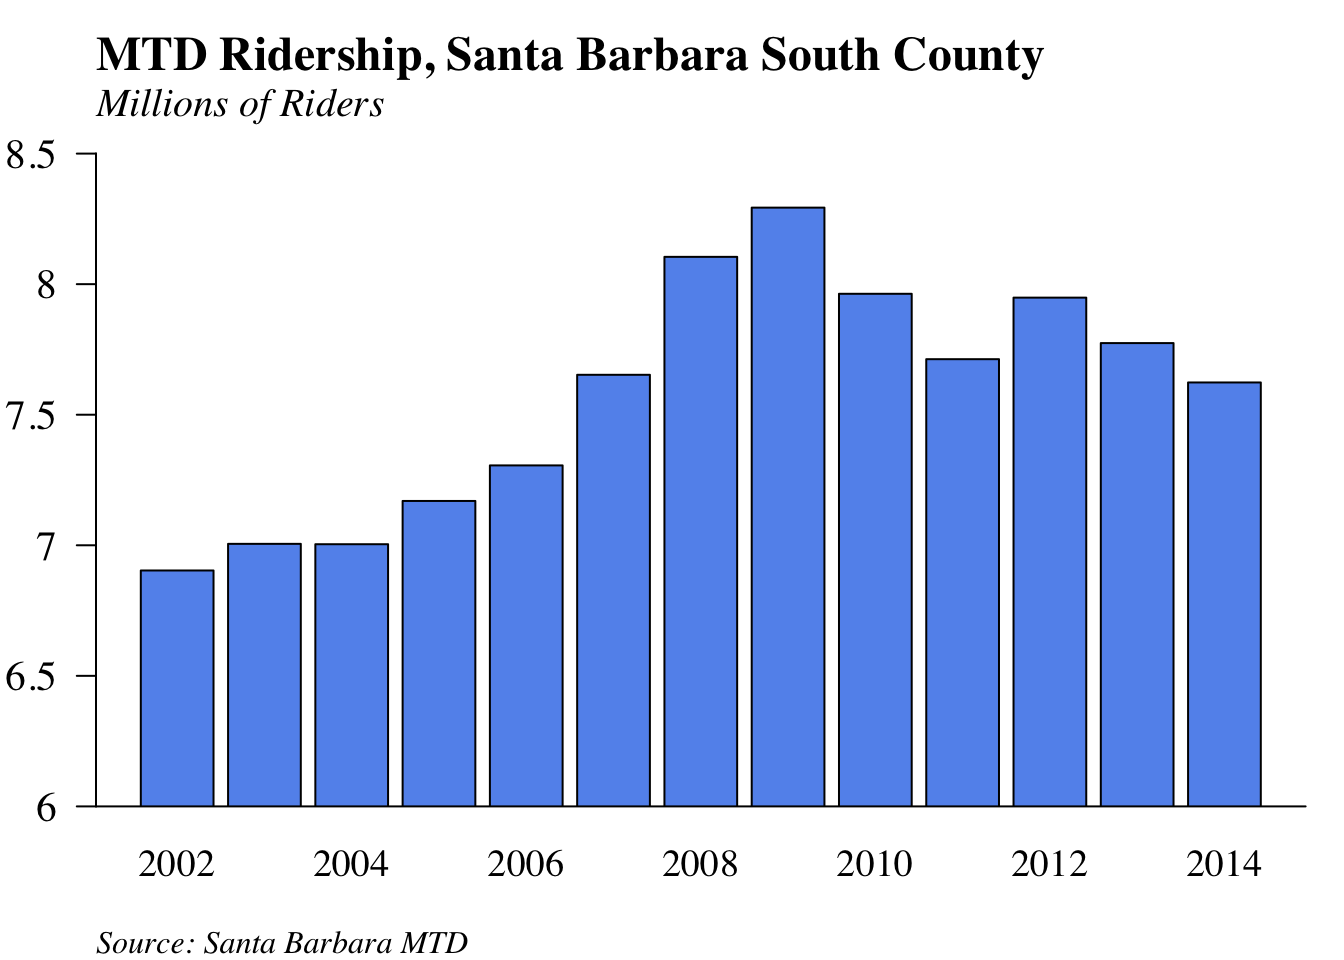
\includegraphics[width=0.95\linewidth]{cip_2019_files/figure-latex/unnamed-chunk-48-1}

\subsubsection*{What is the measure?}\label{what-is-the-measure-23}
\addcontentsline{toc}{subsubsection}{What is the measure?}

The amount of electricity consumed by the Santa Barbara County for
commercial, residential, and industrial purposes, measured in gigawatt
hours. (One gigawatt hour equals one thousand megawatt hours.)

\subsubsection*{Why is it important?}\label{why-is-it-important-22}
\addcontentsline{toc}{subsubsection}{Why is it important?}

Electric energy is a critical commodity, integrated into every aspect of
our lives in our homes and workplaces. However, the production of
electricity may have negative environmental impacts through pollution
and resource use.

\subsubsection*{How are we doing?}\label{how-are-we-doing-29}
\addcontentsline{toc}{subsubsection}{How are we doing?}

Santa Barbara County energy use decreased in 2015, dropping to its
lowest consumption levels in over ten years.

\section*{Mobility}\label{mobility}
\addcontentsline{toc}{section}{Mobility}

\subsection*{MOST WORKERS COMMUTE ALONE BY
CAR}\label{most-workers-commute-alone-by-car}
\addcontentsline{toc}{subsection}{MOST WORKERS COMMUTE ALONE BY CAR}

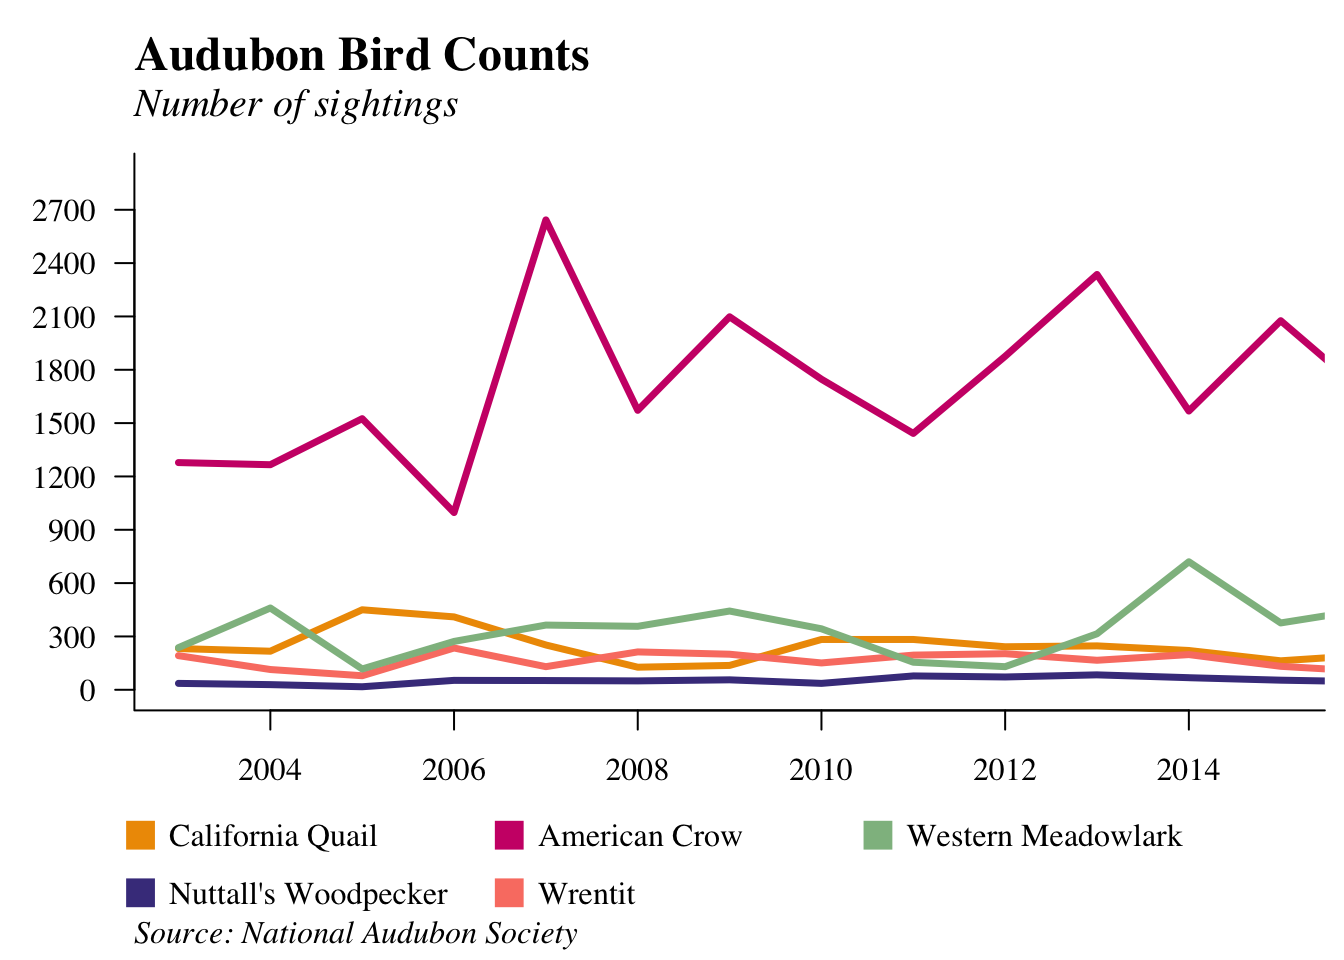
\includegraphics[width=0.95\linewidth]{cip_2019_files/figure-latex/unnamed-chunk-49-1}

\subsubsection*{What is the measure?}\label{what-is-the-measure-24}
\addcontentsline{toc}{subsubsection}{What is the measure?}

The respective percentages of Santa Barbara County residents' means of
transport to work. This data is collected by the United States Census in
the American Community Survey.

\subsubsection*{Why is it important?}\label{why-is-it-important-23}
\addcontentsline{toc}{subsubsection}{Why is it important?}

Mobility reflects the ability of people to get from one place to another
efficiently; consequentially, traffic congestion prevents this from
happening. While traffic congestion has many components -- including the
level of non-commuter automobile use, population, the success of
land-use planning, and the ability of infrastructure improvements to
adapt to changes -- the level of single occupancy vehicle use has a
direct impact on overall traffic congestion.

\subsubsection*{How are we doing?}\label{how-are-we-doing-30}
\addcontentsline{toc}{subsubsection}{How are we doing?}

The majority of workers choose to commute alone by car. The proportion
of these commuters has remained stable over the past five years.

\subsection*{MEAN COMMUTE TIME DECLINES
MARGINALLY}\label{mean-commute-time-declines-marginally}
\addcontentsline{toc}{subsection}{MEAN COMMUTE TIME DECLINES MARGINALLY}

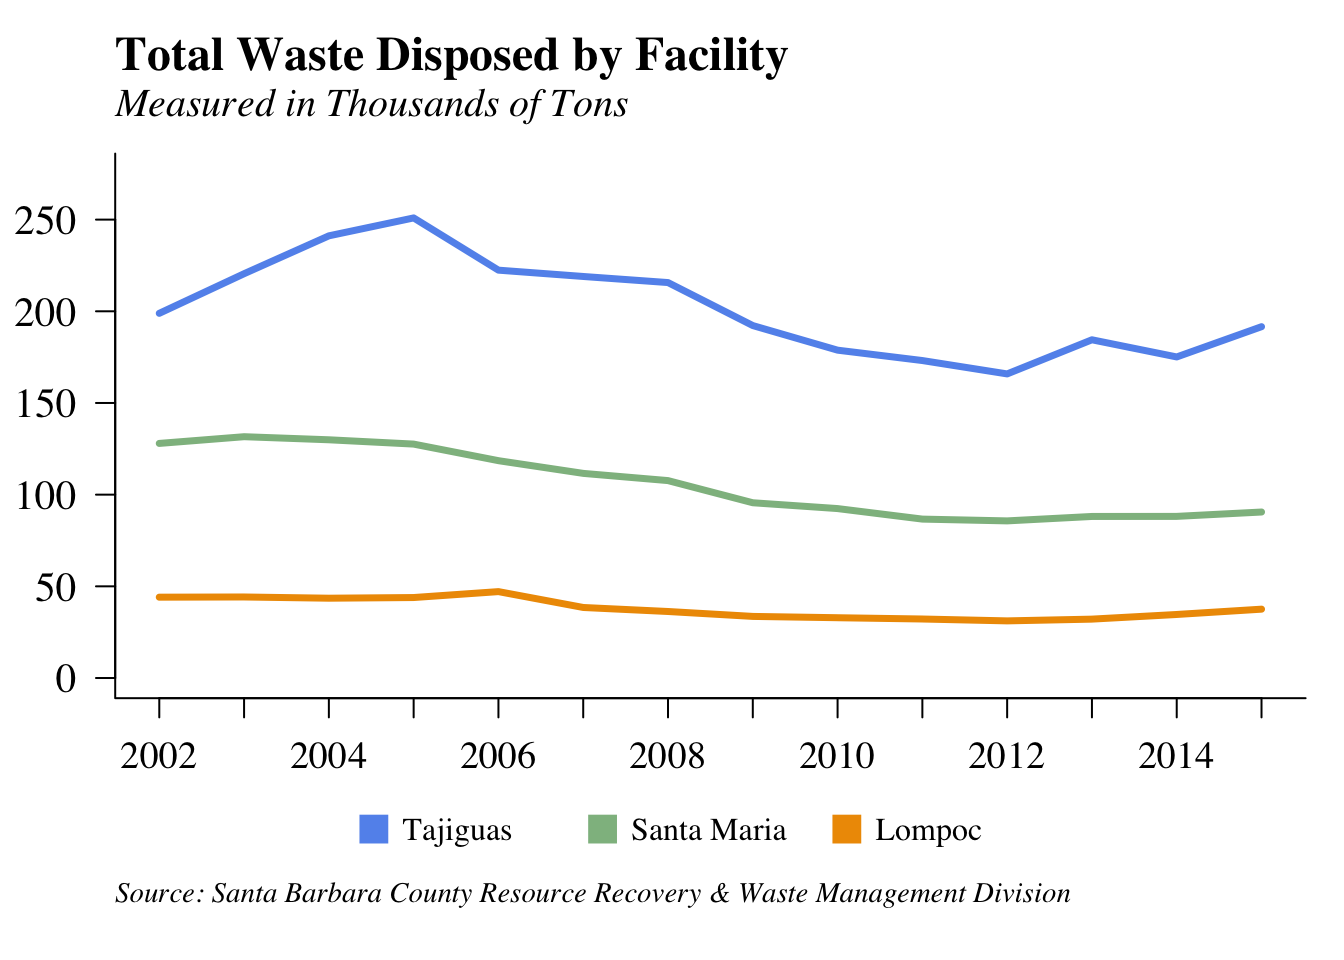
\includegraphics[width=0.95\linewidth]{cip_2019_files/figure-latex/unnamed-chunk-50-1}

\subsubsection*{What is the measure?}\label{what-is-the-measure-25}
\addcontentsline{toc}{subsubsection}{What is the measure?}

The average amount of time it takes a commuter in Santa Barbara County
to travel to work.

\subsubsection*{Why is it important?}\label{why-is-it-important-24}
\addcontentsline{toc}{subsubsection}{Why is it important?}

Commute distances traveled can reveal much about the quality of life and
future trends. Changing commute patterns may indicate a greater
sensitivity toward housing costs and the economy. As the distance
traveled increases, so does pollution, emission levels from automobiles,
and traffic congestion.

\subsubsection*{How are we doing?}\label{how-are-we-doing-31}
\addcontentsline{toc}{subsubsection}{How are we doing?}

The average commute time in 2014 was 18.4 minutes, which is the lowest
average commute time in our data. Over the past ten years, the mean
commute time has peaked at 20.4 minutes.

\subsection*{BUS RIDERSHIP DECREASING}\label{bus-ridership-decreasing}
\addcontentsline{toc}{subsection}{BUS RIDERSHIP DECREASING}

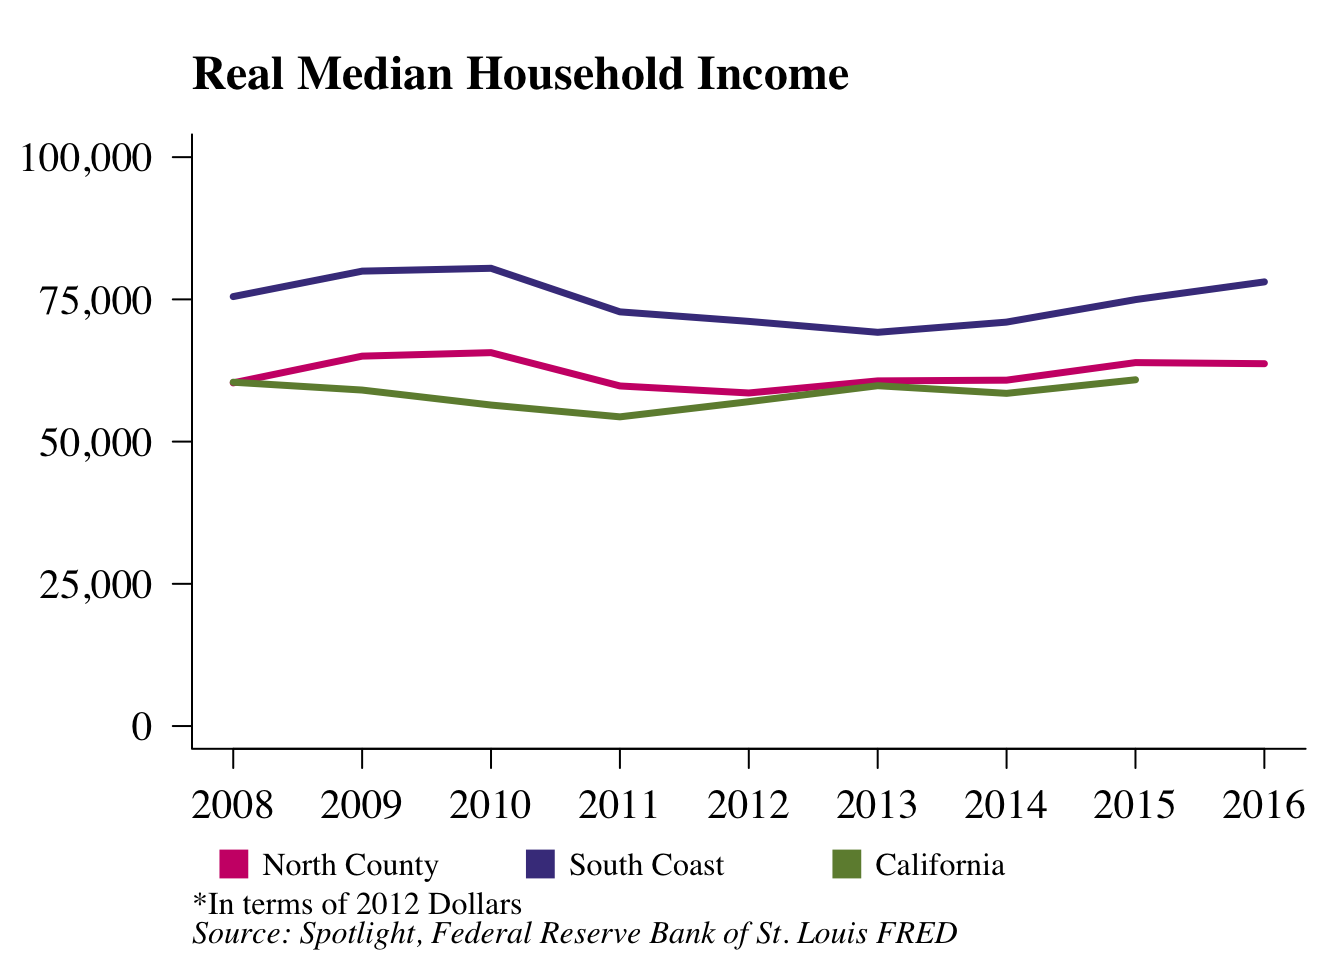
\includegraphics[width=0.95\linewidth]{cip_2019_files/figure-latex/unnamed-chunk-51-1}

\subsubsection*{What is the measure?}\label{what-is-the-measure-26}
\addcontentsline{toc}{subsubsection}{What is the measure?}

The number of bus trips taken in Santa Barbara on Metropolitan Transit
District (MTD) buses. \#\#\#\# Why is it important? \{-\} Buses are
popular means of alternative transportation in Santa Barbara. In many
cases, they are the transportation mode of choice for those who cannot
afford an automobile or are unable to drive. \#\#\#\# How are we doing?
\{-\} Total bus ridership has declined recently to 7.6 million in 2014,
the lowest ridership levels since 2006. Bus ridership levels peaked in
2009 with 8.3 million rides that year.

\subsection*{TRAFFIC VOLUMES STABILIZE OVER LAST FIVE
YEARS}\label{traffic-volumes-stabilize-over-last-five-years}
\addcontentsline{toc}{subsection}{TRAFFIC VOLUMES STABILIZE OVER LAST
FIVE YEARS}

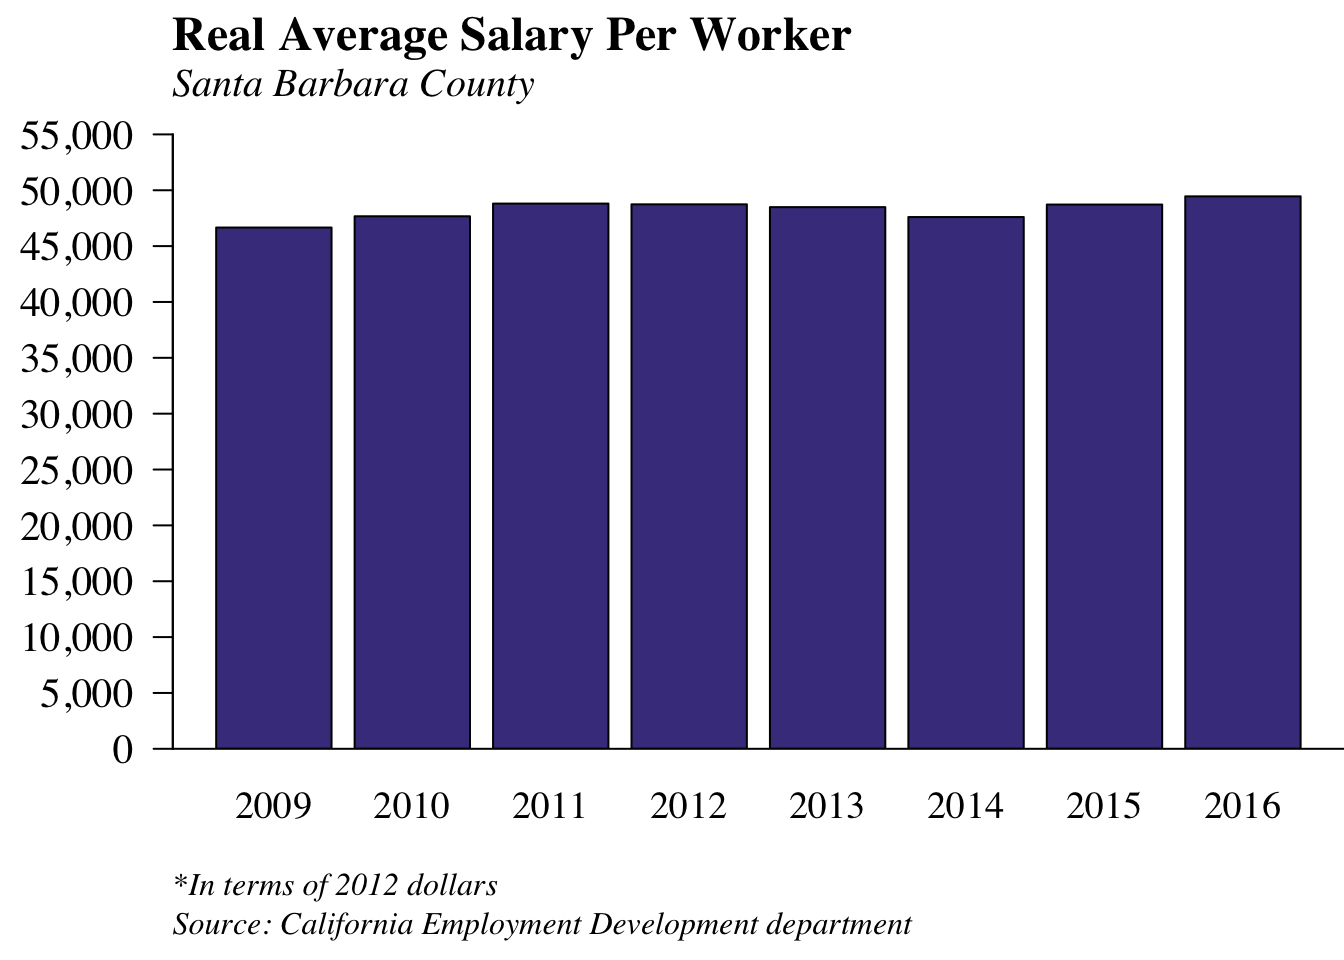
\includegraphics[width=0.95\linewidth]{cip_2019_files/figure-latex/unnamed-chunk-52-1}

\subsubsection*{What is the measure?}\label{what-is-the-measure-27}
\addcontentsline{toc}{subsubsection}{What is the measure?}

The number of cars per day on the freeway counted at three interchanges
in Santa Barbara County. The interchanges are Highway 101 at Fairview,
Las Positas, and Sheffield.

\subsubsection*{Why is it important?}\label{why-is-it-important-25}
\addcontentsline{toc}{subsubsection}{Why is it important?}

Highway 101 is a major roadway in Santa Barbara County, carrying local
traffic, commuters from outside of the area, tourists, and other
traffic. As the major traffic artery in the area, this highway plays an
important role in the mobility of local residents.

\subsubsection*{How are we doing?}\label{how-are-we-doing-32}
\addcontentsline{toc}{subsubsection}{How are we doing?}

As shown on the graph, traffic volume has stayed relatively stable over
the past decade. Las Positas and Sheffield have both seen slight
decreases in their traffic volume, even though all three interchanges
have not seen much change in volume over the last few years.

\section*{Resource Use}\label{resource-use}
\addcontentsline{toc}{section}{Resource Use}

\subsection*{TOTAL WASTE DISPOSED SEES SLIGHT
INCREASE}\label{total-waste-disposed-sees-slight-increase}
\addcontentsline{toc}{subsection}{TOTAL WASTE DISPOSED SEES SLIGHT
INCREASE}

\subsubsection*{What are the measures?}\label{what-are-the-measures-6}
\addcontentsline{toc}{subsubsection}{What are the measures?}

The total tons of waste disposed in the Tajiguas, Santa Maria, and
Lompoc landfills, as well as the amount of green waste and recycling
diverted from the landfills. \#\#\#\# Why is it important? \{-\} Waste
disposal is a major form of urban pollution. Growing populations cause
the total amount of waste to increase. Changes in the local economy,
consumer purchasing decisions, and recycling and composting efforts also
affect the amount of waste. \#\#\#\# How are we doing? \{-\} The total
waste disposed in the Santa Maria and Lompoc landfills increased by
about two thousand tons each, reaching 90,534 and 37,554 tons
respectively. However, the Tajiguas landfill (which serves most of the
South Coast) has seen a larger upward tick in total waste disposed,
moving from 175,099 tons to 191,598 tons. The total amount of green
waste has increased in 2015 from 158 to 160 pounds per capita, whereas
the total recyclables diverted decreased from 100 to 96 pounds per
capita. California currently has a statewide goal of reducing solid
waste by 75 percent by 2020 through recycling, composting, and source
reduction. As of last year, recovery percentage for Santa Barbara County
is 50 percent.

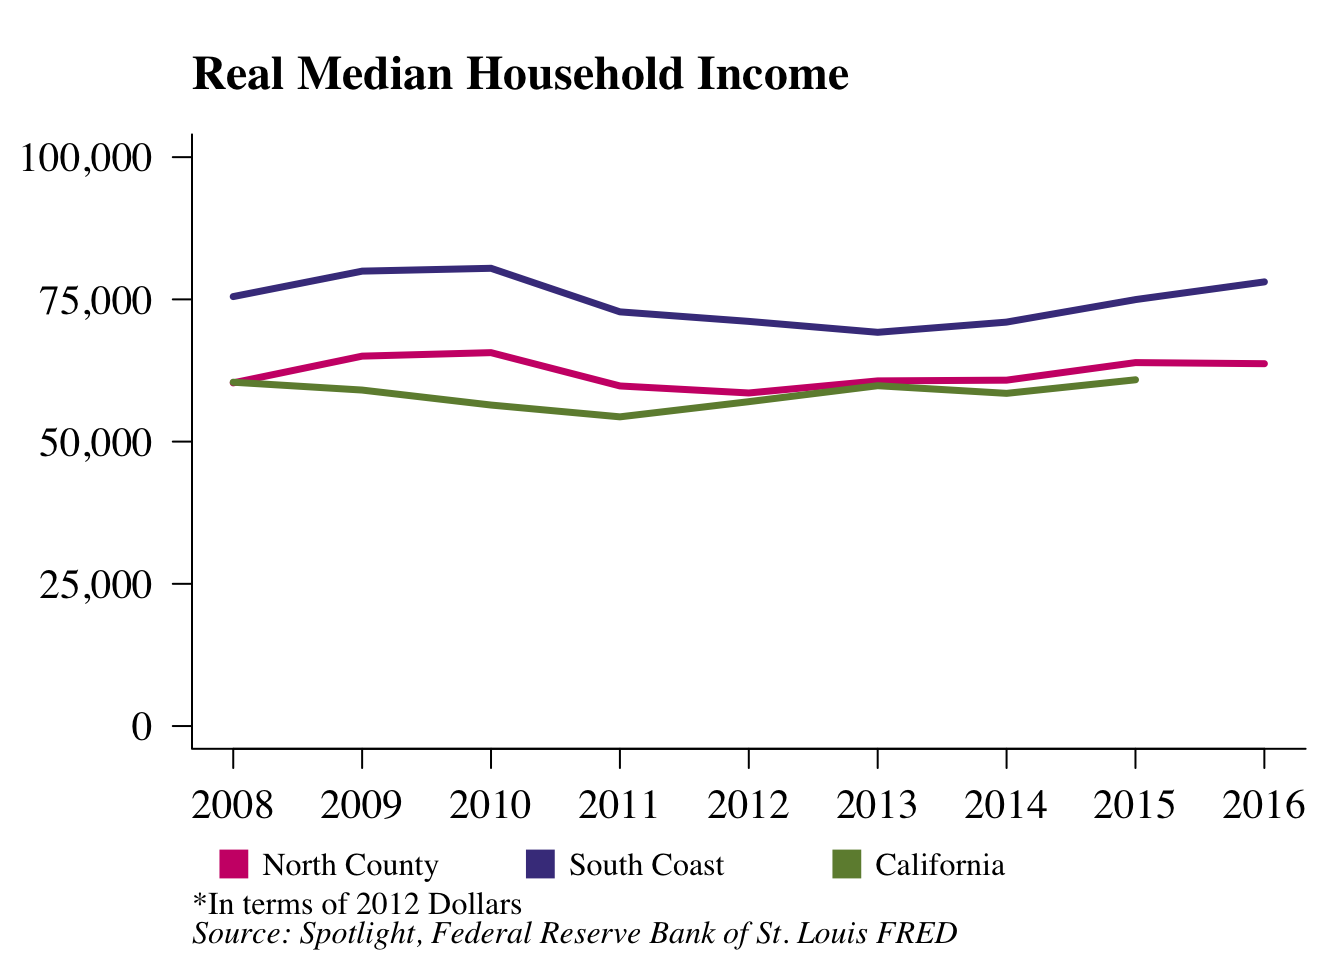
\includegraphics[width=0.95\linewidth]{cip_2019_files/figure-latex/unnamed-chunk-53-1}

\includegraphics[width=0.95\linewidth]{cip_2019_files/figure-latex/unnamed-chunk-54-1}

\begin{center}\includegraphics[width=0.5\linewidth]{cip_2019_files/figure-latex/unnamed-chunk-55-1} \end{center}

\section*{Nature}\label{nature}
\addcontentsline{toc}{section}{Nature}

\subsection*{TOTAL BIRD COUNT EXPERIENCES A
DECLINE}\label{total-bird-count-experiences-a-decline}
\addcontentsline{toc}{subsection}{TOTAL BIRD COUNT EXPERIENCES A
DECLINE}

\includegraphics[width=0.95\linewidth]{cip_2019_files/figure-latex/unnamed-chunk-56-1}

\subsubsection*{What is the measure?}\label{what-is-the-measure-28}
\addcontentsline{toc}{subsubsection}{What is the measure?}

The results of the Audobon Society's annual Christmas Bird Count for
five species. The bird count is designed as a measure of the diversity
of bird species, but it can also be used as a rough indicator of how
well bird species are thriving.

Five common species are reported - the California Quail, the Nuttall's
Woodpecker, the American Crow, the Wrentit, and the Western Meadowlark.
All of these species are resident birds, living in different local
habitats.

\subsubsection*{Why is it important?}\label{why-is-it-important-26}
\addcontentsline{toc}{subsubsection}{Why is it important?}

Bird populations are an important part of out local ecosystem, and
generally reflect its overall health. Changes in the bird count can
reflect changes in habitat or other shifts in local environment.

\subsubsection*{How are we doing?}\label{how-are-we-doing-33}
\addcontentsline{toc}{subsubsection}{How are we doing?}

For the past decade, the number of Nuttall's Woodpeckers, Wrentits, and
Western Meadowlarks have generally declined. These species have
decreased mainly due to the loss of local chapparral and woodlands.
However, the number of sightings of American Crows has seen a 36 percent
increase from 2005 to 2015.

In 2015, Western Meadowlarks sightings fell dramatically from 720 to
376, a 47 percent decline. This decrease is surprising considering the
129 percent increase seen from 2013 to 2014. Similar to the Western
Meadowlarks, the number of California Quails also fell by 26 percent
moving from 2014 to 2015 after increasing considerably the years before.

The sightings of Wrentits and Nuttall's Woodpecker's generally stayed
the same, although remaining on a downward trend. As most of the species
decline, the number of American Crows sightings continues to grow,
representing more than half of the total bird count.

\chapter*{Economic}\label{economic}
\addcontentsline{toc}{chapter}{Economic}

\section*{Standard of Living}\label{standard-of-living}
\addcontentsline{toc}{section}{Standard of Living}

\section*{Job Quality and Quantity}\label{job-quality-and-quantity}
\addcontentsline{toc}{section}{Job Quality and Quantity}

\section*{Housing Affordability}\label{housing-affordability}
\addcontentsline{toc}{section}{Housing Affordability}

\section*{Business Vitality}\label{business-vitality}
\addcontentsline{toc}{section}{Business Vitality}

\chapter{Final Words}\label{final-words}

We have finished a nice book.

\bibliography{book.bib,packages.bib}


\end{document}
